%
% Bachelor Thesis
% ---------------
%
% Master File
%
% Andreas Stöckel, 2013
%

\documentclass[a4paper,11pt]{memoir}
\usepackage[utf8]{inputenc}
\usepackage{amsmath}
\usepackage{amsfonts}
\usepackage{amssymb}
\usepackage{amsthm}
\usepackage{nicefrac}
\usepackage{graphicx}
\usepackage[pdftex,
            pdfauthor={Andreas Stoeckel},
            pdftitle={Realtime obstacle detection from optical flow in panoramic images},
            pdfsubject={Visual navigation},
            pdfkeywords={obstacle detection, optical flow, panoramic images, omnidirectional images, realtime, depth estimation, structure from motion}
            ]{hyperref}
\usepackage[round,colon]{natbib}
\usepackage{rotating}
\usepackage{algorithm}
\usepackage{algpseudocode}
%\usepackage{microtype}
\usepackage{dpfloat}
\usepackage{array}

% Code
\usepackage{xcolor}
\usepackage{listings}

\definecolor{listing}{rgb}{0.95, 0.95, 0.95}
\definecolor{lst_green}{rgb}{0, 0.5, 0}
\definecolor{lst_blue}{rgb}{0, 0, 0.5}
\definecolor{lst_red}{rgb}{0.5, 0.3, 0.1}
\definecolor{lst_gray}{rgb}{0.35, 0.35, 0.35}

\lstset{
  language=c,
  tabsize=2,
  breaklines=true,
  postbreak=\raisebox{0ex}[0ex][0ex]{\ensuremath{\hookrightarrow}},
  basicstyle=\small\ttfamily,
  keywordstyle=\color{lst_blue},
  keywordstyle=[2]\color{lst_red},
  commentstyle=\color{lst_gray},
  morekeywords={\_\_m128i},
  keywords=[2]{\_mm\_load\_si128,\_mm\_store\_si128,\_mm\_shuffle\_epi8,\_mm\_maddubs\_epi16,\_mm\_or\_si128,\_mm\_srai\_epi16,\_mm\_packus\_epi16,\_mm\_set\_epi8,
  \_mm\_loadu\_si128,\_mm\_srli\_epi16,\_mm\_abs\_epi16,\_mm\_cmpeq\_epi16,\_mm\_sub\_epi16,\_mm\_storeu\_si128,\_mm\_adds\_epi16}
}

% Description labels
\renewcommand*{\descriptionlabel}[1]{\hspace\labelsep\normalfont\itshape #1}


% Page layout
\setstocksize{29.7cm}{21cm}
\settrimmedsize{\stockheight}{\stockwidth}{*}
\setlrmarginsandblock{4.5cm}{3.5cm}{*}
\setulmarginsandblock{4.5cm}{4.5cm}{*}
\checkandfixthelayout
\pagestyle{ruled}

% Numbering depth (number subsections)
\setsecnumdepth{subsection}

% Subfigures
\newsubfloat{figure}

% Title page
\pretitle{
\begin{center}
	\Large
	Universität Bielefeld\\
	Technische Fakultät\\
	AG Technische Informatik
	\vspace{1.25cm}\\
	\textsc{Bachelorarbeit}
	\vspace{0.75cm}\\
\end{center}
\hrulefill
\begin{center}\scshape\Huge}
\posttitle{\end{center}\hrulefill}

\preauthor{\vspace{0.5cm}\begin{center}\Large}
\postauthor{\\\vspace{0.25cm}
\end{center}}

\predate{\begin{center}\Large}
\postdate{\vspace{1cm}\\
	\normalsize
	Im Studiengang\\
	Kognitive Informatik\\
	\vspace{1cm}
	\textbf{Gutachter}\\
	M.Sc.\ Michael Horst\\
	M.Sc.\ David Fleer
	\end{center}}

\captionstyle{\small}
\captionnamefont{\scshape}

\usepackage[]{todonotes}
%\newcommand{\todo}[2][\empty]{}
%\newcommand{\listoftodos}{}{}

%
% Mathematical Command Definitions
% Andreas Stöckel
%

\newcommand{\nok}[2]{{\left(\begin{matrix}{#1}\\{#2}\end{matrix}\right)}}
\newcommand{\snok}[2]{{\left(\begin{smallmatrix}{#1}\\{#2}\end{smallmatrix}\right)}}
\newcommand{\N}{{\mathbb{N}}}
\newcommand{\Q}{{\mathbb{Q}}}
\newcommand{\R}{{\mathbb{R}}}
\newcommand{\Z}{{\mathbb{Z}}}
\newcommand{\C}{{\mathbb{C}}}
\newcommand{\E}{{\mathbb{E}}}

\newcommand{\Var}{{\mathrm{Var}}}
\newcommand{\p}{\mathbf{p}}

\renewcommand{\epsilon}{\varepsilon}
\renewcommand{\phi}{\varphi}
\renewcommand{\theta}{\vartheta}
\renewcommand{\complement}{\mathsf{C}}

\newcommand{\prodset}[2]{\overset{#2}{\underset{#1}{\prod}}}

\newcommand{\lsp}[1]{{\mathcal{L}\left({#1}\right)}}
\newcommand{\stf}[1]{{\mathcal{T}\left({#1}\right)}}

\newcommand{\limn}{{\lim_{n \to \infty}}}
\newcommand{\limx}{{\lim_{x \to x_0}}}
\newcommand{\limm}{\;{\overset{n \to \infty}\longrightarrow}\;}
\newcommand{\smbox}[1]{{\text{\small{{#1}}}}}

\newcommand{\nfolge}[1]{{\left({#1}_n\right)_{n \in \N}}}

\newcommand{\twoway}[2]{{$\left\{\begin{matrix}\text{#1}\\\text{#2}\end{matrix}\right\}$}}

\newcommand{\mapping}[5]{{\begin{array}{rrcl}{#1}: & {#2} & \longrightarrow & {#3} \\ & {#4} & \mapsto & {#5}\end{array}\;}}

\newcommand{\supr}[2]{\ensuremath{\left\lVert#1\right\lVert_{#2}}}

\newcommand{\indy}[1]{\mathfrak{1}_{#1}}

\newcommand{\pbox}[1]{\parbox[tc]{2cm}{\small{#1}}}

\newcommand{\sumni}{\sum_{n=0}^\infty}
\newcommand{\intab}{\int_a^b}

\newcommand{\fbeg}[2]{\left.{#1}\right|_{#2}}

\newcommand{\eqs}{\hat=}

\newcommand{\konj}[1]{\overline{#1}}

%\renewcommand{\i}{\mathtt{i}}

\newcommand{\Hom}{\mathrm{Hom}}

\newcommand{\begmat}{\left( \left. \begin{matrix}}
\newcommand{\vlimat}{\end{matrix} \hspace{0.1cm}\right|  \left. \begin{matrix}}
\newcommand{\finmat}{\end{matrix}\right. \right)}

\newcommand{\sbegmat}{\left( \left. \begin{smallmatrix}}
\newcommand{\svlimat}{\end{smallmatrix} \hspace{0.1cm}\right|  \left. \begin{smallmatrix}}
\newcommand{\sfinmat}{\end{smallmatrix}\right. \right)}

\newcommand{\isom}{\overset\sim=}

\newcommand{\arsin}{\mathrm{arsin}}
\DeclareMathOperator{\atantwo}{arctan2}
\newcommand{\im}{\mathrm{im}}
\newcommand{\Rg}{\mathrm{Rg}}
\newcommand{\id}{\mathrm{id}}
\renewcommand{\ker}{\mathrm{ker}}
\newcommand{\tr}{\mathrm{tr}}
\newcommand{\Eig}{\mathrm{Eig}}

\newcommand{\sign}{\mathrm{sign}}

\newcommand{\argmin}{\operatornamewithlimits{argmin}}
\newcommand{\argmax}{\operatornamewithlimits{argmax}}

\newcommand{\img}[1]{\mathbf{#1}}
\newcommand{\imgpix}[1]{\mathbf{#1}_{\mathbf{P}}}
\newcommand{\imgang}[1]{\mathbf{#1}_{\mathbf{S}}}

\let\oldvec=\vec
\renewcommand{\vec}[1]{{\text{$\oldvec{#1}$}}}

\theoremstyle{remark}
\newtheorem*{derivation}{Derivation}

\newtheorem{theorem}{Theorem}

\title{Realtime obstacle detection from optical flow in panoramic images}
\author{Andreas Stöckel}
\date{5. September 2013}

\makeatletter
\let\insertdate\@date
\let\insertauthor\@author
\makeatother

\begin{document}

\begin{titlingpage}
	\maketitle
	\thispagestyle{empty}
	\clearpage
	\thispagestyle{empty}
	~~\vspace{15.5cm}\\
	\textbf{Danksagung}\vspace{0.75cm}\\
	Danke an meine Betreuer Michael Horst und David Fleer für das widerstandslose Ertragen meiner Berichte über Probleme, die sich im Anschluss daran meist von selbst lösten, zündende Ideen, sowie das Korrekturlesen des Manuskripts. Dank gilt natürlich auch meiner Familie -- insbesondere meinen Eltern -- dafür, mein Exil fernab der Heimat so erträglich wie irgend möglich zu gestalten. Abschließend gilt mein besonderer Dank Herrn Prof.\ Möller für den \textit{Earl Grey} Tee, dessen Superkräfte mich auch zu nachtschlafender Zeit noch arbeiten ließen.
\end{titlingpage}

\setcounter{tocdepth}{2}
\tableofcontents*

%\chapter*{Todo}
%\listoftodos

\chapter*{Summary}
\addcontentsline{toc}{chapter}{Summary}

An important component of mobile robot navigation is obstacle detection. For this purpose, the target robot platform is equipped with a set of static laser diodes and an omnidirectional camera. The usage of only four diodes at a time in conjunction with slow temporal sampling results in a relatively coarse environmental coverage, which causes small and slim objects (like legs of tables or chairs) to be often missed.

A previously developed algorithm is capable of detecting obstacles by analyzing time series of spherical panoramic images using implicit optical flow estimation. The goal of this thesis is to lay the theoretical foundations of the algorithm and to present performance optimizations allowing real-time operation on an embedded system. Moreover, measures for the obstacle detection performance in simulated test runs are developed.

Performance optimization is achieved by a resolution pyramid with coarse-to-fine refinement in the optical flow estimation step, motion field precalculation, as well as the use of single instruction multiple data (SIMD) instruction set extensions in the implementation.

The final implementation fully satisfies the real-time constraint, typically requiring less than $30\,\mathrm{ms}$ for an obstacle detection step on the target system. While tests in simulated environments show that the algorithm is capable of mean obstacle detection errors smaller than $0.06\,\mathrm{m}$, the real-world performance heavily depends on the quality of the input and especially on correct robot orientation estimates.

\chapter{Introduction}

In the last three decades a vast number of techniques for obstacle detection and evasion in mobile robots have been developed. While classical approaches include active range sensors, advancements in imaging hardware and processing power led to approaches which solely rely on visual information.

This chapter provides an overview of the particular obstacle detection problem that had to be solved, as well as an outline and evaluation of already existing approaches, finally leading to the actual method presented in this thesis.

\section{Motivation}

\begin{figure}[t]
 \begin{center}
  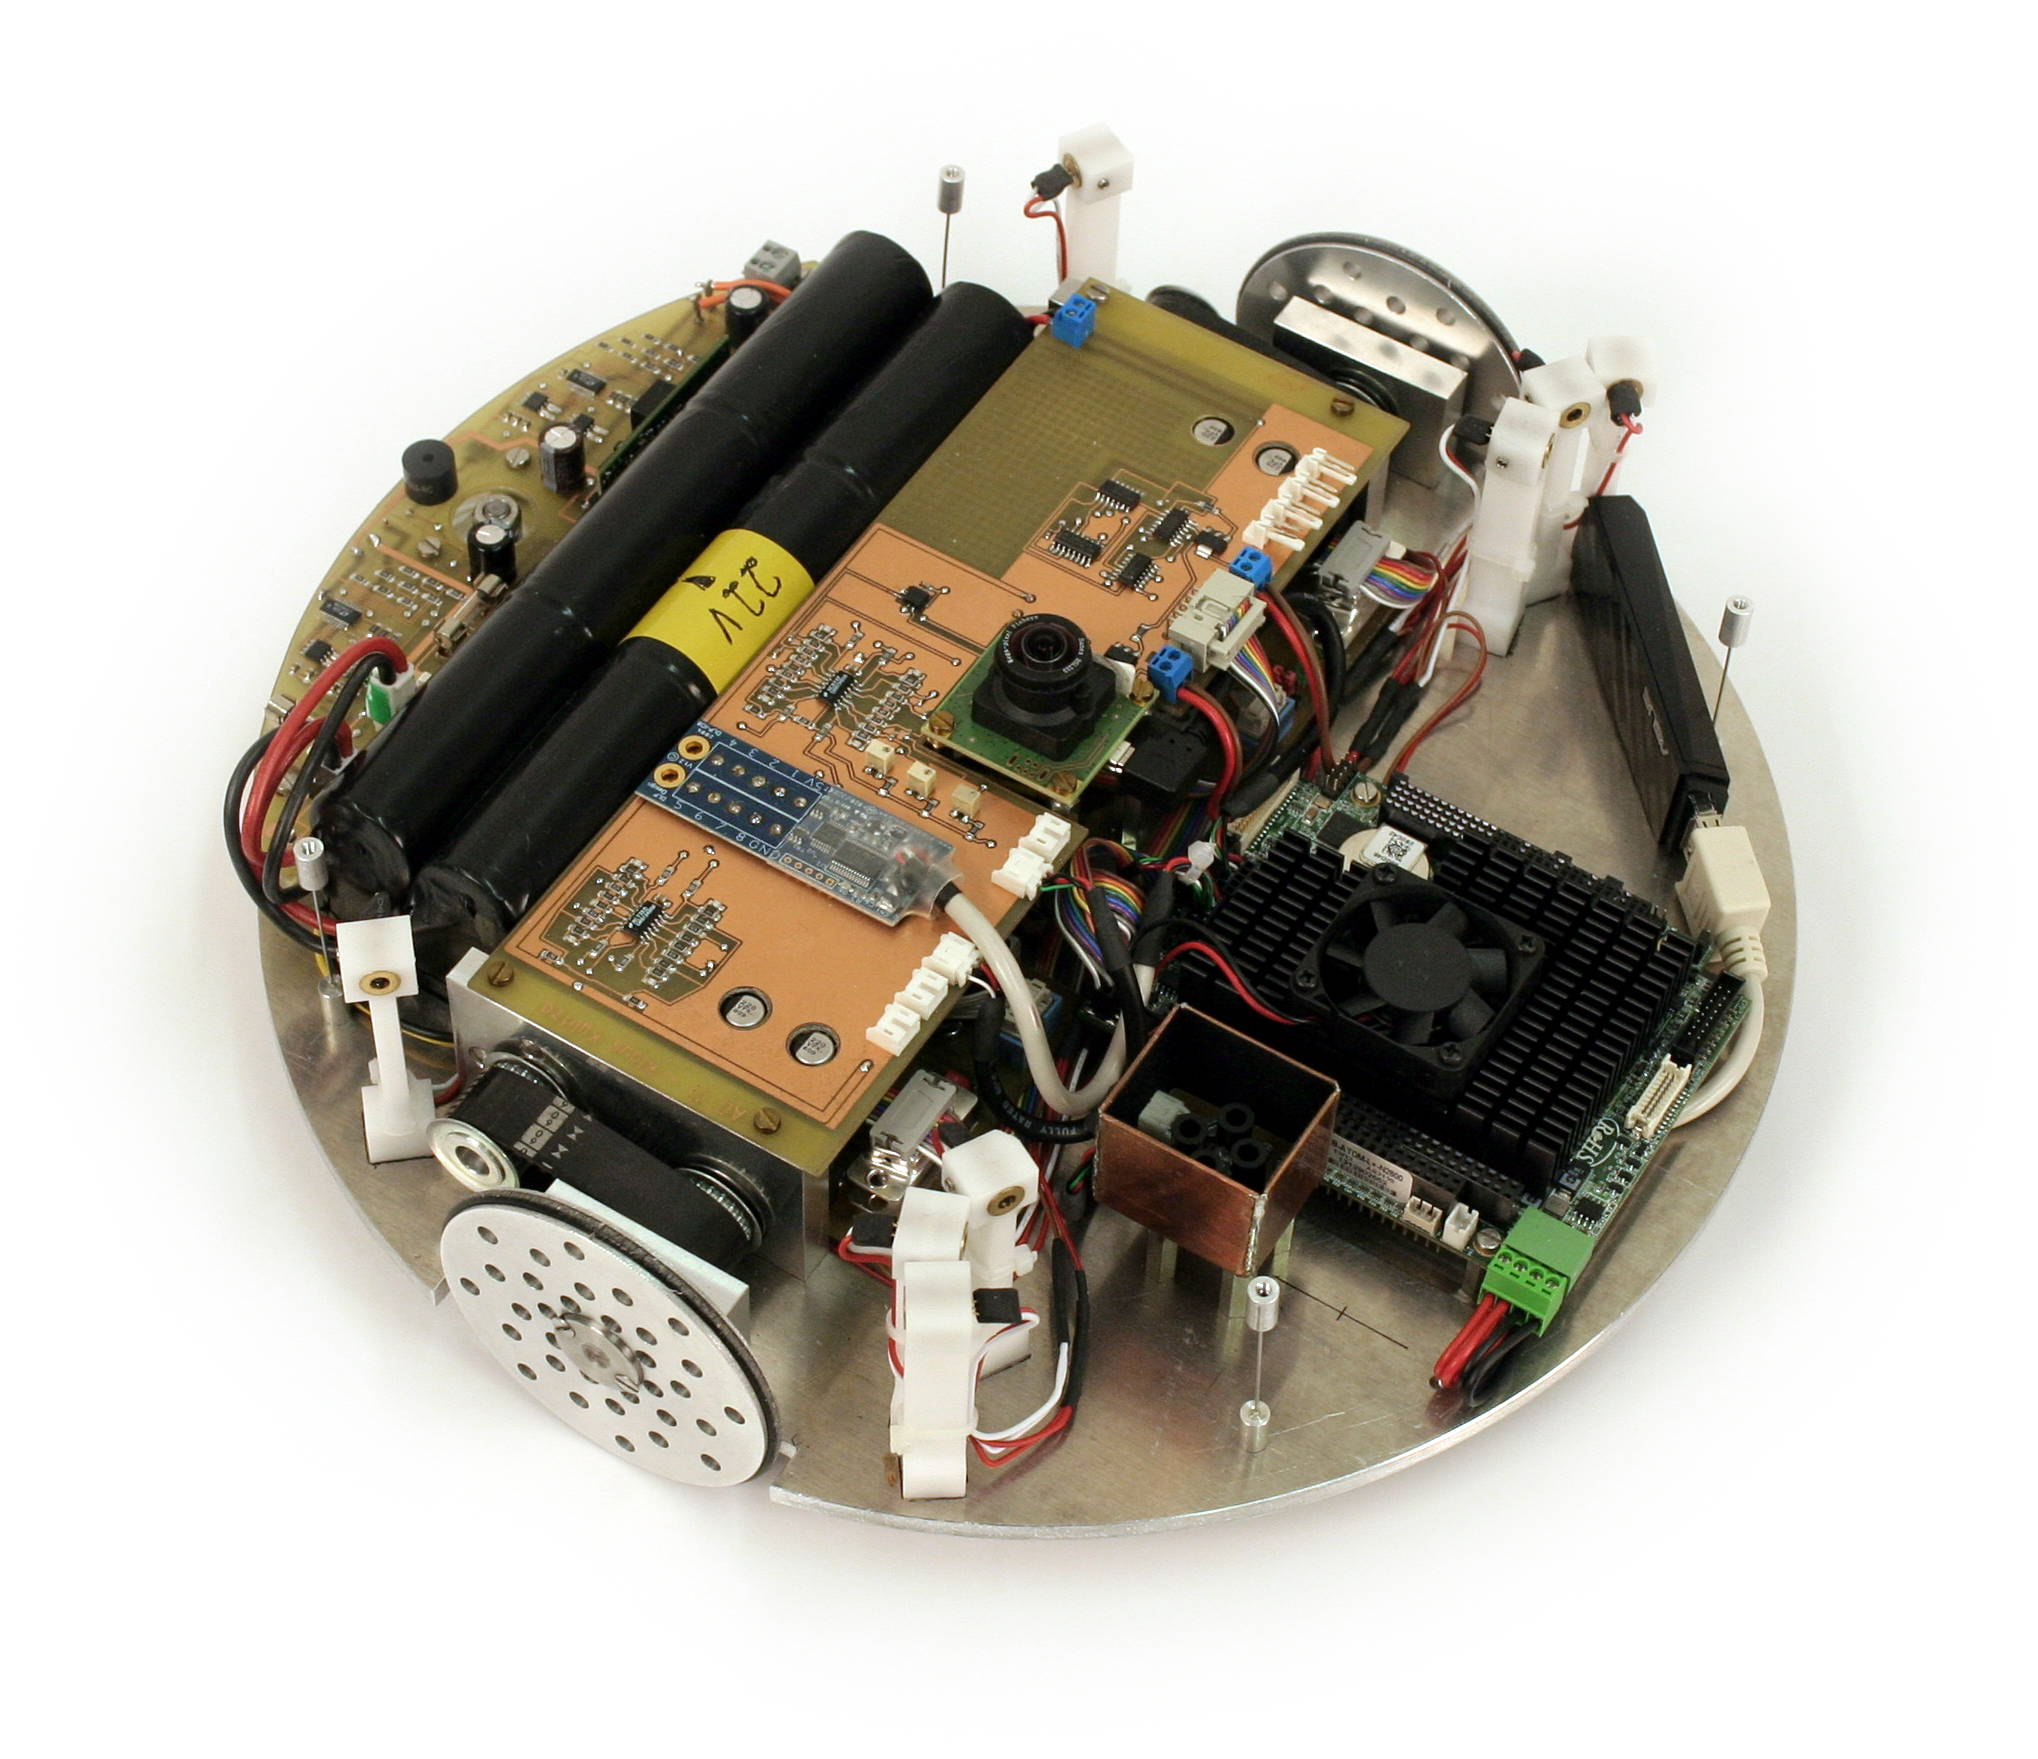
\includegraphics[width=0.8\textwidth]{media/nr6.jpg}
 \end{center}
 \caption{Photo of the robot platform (in-house development) as used in the experiments. One can see the eight laser diodes (mounted at the white holders) used for the coarse obstacle detection as well as the fisheye camera in the center of the platform and the on-board computer at the right side of the image. The radius of the entire system (including the cover not shown) is about $35\;\mathrm{cm}$, the top of the camera lens is located about $10\;\mathrm{cm}$ above the ground.}
 \label{fig:nr5}
\end{figure}

Obstacle detection and avoidance are crucial to most autonomous mobile systems, both biological and robotic. While mandatory for systems moving at high velocities in order to avoid physical damage, long-range obstacle detection is still a necessity for efficient navigation and route planning in applications like consumer-grade cleaning robots.

The target robot platform --- an in-house development inspired by such cleaning robots (see figure \ref{fig:nr5}) --- carries a set of eight static lasers diodes which are used for obstacle detection. The detection is performed by triangulating the laser points as they appear in an omnidirectional camera image. The usage of only four diodes at a time in conjunction with slow temporal sampling results in a relatively coarse environmental coverage, which likely causes small and slim objects to be missed.

Classical approaches to obstacle detection on mobile robots include sonar sensors and laser scanners, while more recent developments include time-of-flight cameras and structured light sensors \citep[chapter 4.1.9 ``Active ranging'', p. 125ff.]{AutonomousMobileRobots}. While laser scanners in particular provide a high spatial resolution, these solutions are specialized hardware components which might not be suitable for budget-constrained consumer devices. However, commercially available cleaning robots that employ laser scanner based obstacle detection exist\footnote{According to the manufacturer, laser scanner based obstacle detection is employed in their \textit{Neato} robot vacuum cleaner series (see \url{http://www.neatorobotics.com/}). Yet the laser scanner used here might not measure time of flight, but may instead be based on triangulation.}. Furthermore space, payload and electrical power restrictions can often force the hardware to be as simple and small as possible.

The availability of low-cost imaging hardware (partially caused by the widespread adaption of cameras in day-to-day electronic devices) and the emergence of small, powerful microprocessors with low energy footprint allow for cost-effective integration of image processing systems into mobile robots. Therefore a monochrome, upward directed camera equipped with a fisheye lens, allowing omnidirectional vision, is already built into the robot platform and --- besides the coarse laser based obstacle detection --- utilized for navigation using min-warping \citep{own_moeller10_1,own_hillen_13_1}.

The goal of this thesis is to deduce an obstacle detection algorithm from a fundamental optical flow equation and finally to provide a real-time solution capable of exploiting the visual information provided by the visual sensor. Obstacle detection is thus turned from a hardware into a mere software problem.

\section{Special requirements}

\label{sec:intro_special}

In order to allow real-time operation of the entire robot, the obstacle detection algorithm must stay within a certain time budget. As the algorithm has to run along numerous other processes and a new image is captured approximately every $200\,\mathrm{ms}$, the execution time of the obstacle detection method should stay well below $50\,\mathrm{ms}$ on an embedded Intel\textregistered\ Atom\texttrademark\ N2600 dual core CPU running at $1{.}60 \, \mathrm{GHz}$.

Another requirement concerns the vertical range in which obstacles need to be detected: The robot only has a height of about $10\;\mathrm{cm}$, hence obstacles lying far above that height do not need to be detected. In fact, detecting such obstacles (at least without height information) would be counterproductive, as it might prevent the robot from driving beneath furniture.

The requirements are relaxed by the fact that the robot is aimed at domestic indoor use, which allows to assume a relatively static world and a mostly even ground.

\section{Existing solutions}

\label{sec:existing_solutions}

Vision based obstacle detection is an active research area. Binocular vision is an approach often used in applications for which reliable obstacle detection in non-static worlds or in conditions without ego-motion is mandatory (for example automotive applications as in \citealp{650851}).

Fewer solutions exist for omnidirectional, monocular vision. The underlying idea of these approaches is to exploit the parallax information present in subsequent images captured under motion: Near objects show a relatively large displacement and can thus be detected.

The following list contains a selection of approaches suitable for the present camera setup:
\begin{description}
 \item[Direct analysis of non-sparse optical flow:] In this approach, non-sparse optical flow is estimated from a time series of images. The flow field is then directly fed into the motor controller in order to avoid obstacles. This approach can be biologically motivated, as for example insect flight is believed to be controlled by optical flow \citep{Egelhaaf:2009}. Early experiments with optical flow and flying robots have shown that this direct form of motor control is indeed practical \citep{doi:10.1117/12.131575}.

 \item[Free space detection:] As above optical flow is estimated from a time series of images and compared to the expected movement of the ground surface. Instead of direct motor control, free space regions with no obstacles are detected by analyzing the difference between the expected and measured flow vector field \citep{yoshizaki:inria-00325322}.

 \item[Feature-based optical flow and obstacle detection:] A sparse flow field is created by matching corresponding image regions in a time series of input images. This matching may be performed using either sparse optical flow estimation techniques and/or feature detectors like SIFT \citep{Lowe04distinctiveimage}. Single high velocity flow vectors then correspond to near obstacles.

 This method is for example described in a paper by \citet{Low05obstacledetection}, where an one-dimensional polar obstacle map (comparable to those obtained from a laser scanner) is built from a ``flow vector length to distance'' estimate.

 \item[Obstacles from depth:] Given the presence of a depth map which is reconstructed from the input images, classical approaches for robot navigation \citep[][chapters 5 and 6]{AutonomousMobileRobots} can be employed.

 Methods for depth reconstruction in monocular vision include \textit{shape from texture} and \textit{shape from shading}. Here depth information is reconstructed from still images under assumptions about texture distortion or lighting \citep{buelthoff1991shape}. Moreover, machine learning approaches can be applied to depth recognition in still images \citep{depthStill}.

 Reconstructing depth from a series of images captured at slightly different positions is called \textit{structure from motion}. Here a correspondence between feature points from at least two images is established. Besides performing depth reconstruction, the camera motion is estimated \citep[see][chapter 4.2.6 ``Structure from motion'', p. 181ff.]{AutonomousMobileRobots}.

 An example for \textit{structure from motion} in omnidirectional images on mobile robots can be found in \citet{kawanishi2013parallel}, where parallel vertical lines are extracted as features in order to allow operation in textureless artificial environments.
\end{description}

\section{Algorithm overview}

In this section the approaches listed above are evaluated, followed by a brief summary of the solution presented in this thesis.

\subsection{Limitations of the approaches presented above}

The algorithm presented in this thesis follows the \textit{obstacles from depth} design scheme:

An insect-like, direct control scheme is not suitable for efficient, pre-planned trajectories. Free space detection as proposed by \citeauthor{yoshizaki:inria-00325322} cannot be used, as the omnidirectional camera on the robot platform does not cover the range below the image horizon and thus does not see the ground. In fact, it is noteworthy that many algorithms for obstacle detection in monocular, omnidirectional vision systems (including those mentioned above) are designed for a catadioptric camera system mounted on top of the robot, which allows to perceive the ground plane \citep{yasushi1999omnidirectional,kim2007omnidirectional}.

Feature-based approaches were also discarded, as preceding tests have shown that in usual domestic environments only few points of interest are present in the narrow ($\leq 10^\circ$) range above the image horizon, which is critical for obstacle detection.

Most \textit{structure from motion} methods also use feature points for depth reconstruction and as mentioned above try to estimate the camera motion between the images. Yet as the robot knows its current velocity from the odometry data, this motion information is not required. In addition these techniques --- including shape from shading and machine learning approaches --- may not be suitable for the real-time constraints given on an embedded system.


\subsection{General idea}

\begin{figure}[p]
 \begin{center}
  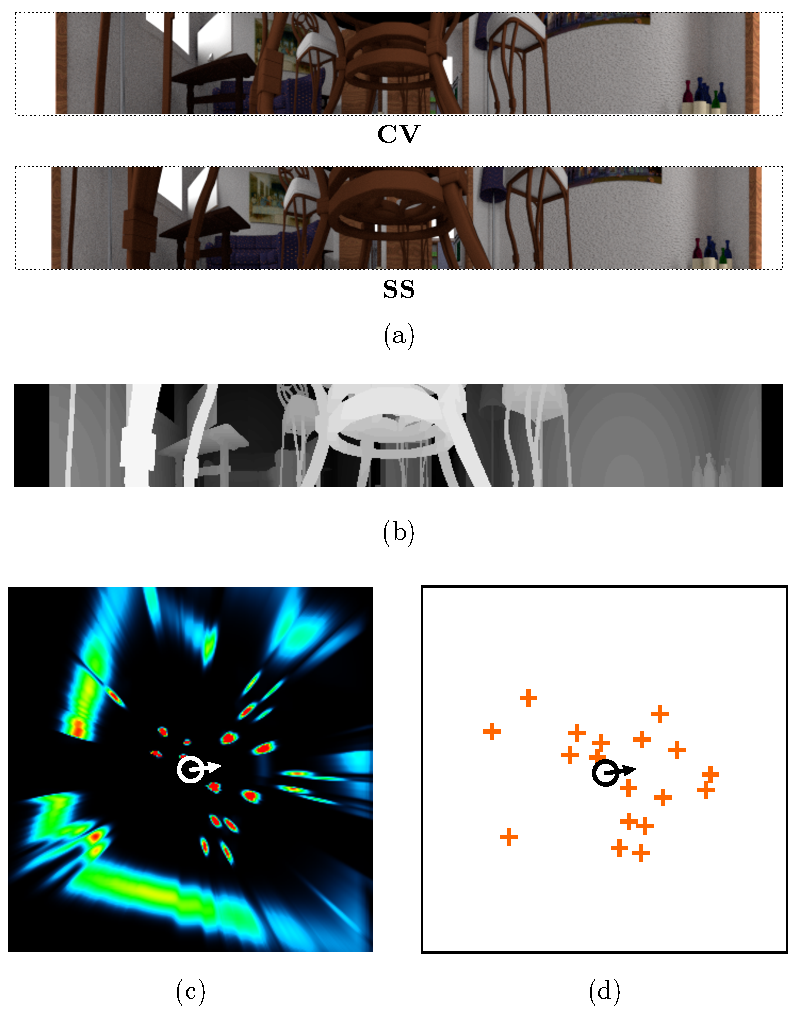
\includegraphics[width=0.8\textwidth]{media/general_idea2.pdf}
 \end{center}
 \caption{Conceptual overview of the stages in the obstacle detection algorithm:
 (a) A pair of panoramic input images (current view $\img{CV}$ and snapshot $\img{SS}$) is given (the actual images are monochrome). (b) Estimation of a depth map containing the distance for every pixel (image shows the ground truth). (c) The uncertainty distribution of each reconstructed pixel is accumulated in a top-down projected local environment map. (d) Clusters in the map with high density values are returned as obstacle points.}
 \label{fig:general_idea}
\end{figure}

Figure \ref{fig:general_idea} shows a short summary of the general idea of the algorithm: The depth reconstruction is performed by implicitly estimating optical flow. This flow estimation is accelerated by utilizing as much prior knowledge as applicable, including the motion information returned from the odometry sensors. Once the depth has been reconstructed, the resulting landmark points are projected onto a local top-down environment map in which the probability distributions accompanying each reconstructed surface point are accumulated. If a certain threshold is exceeded, the corresponding map region is emitted as an obstacle point.

\chapter{Algorithm description}

This chapter describes the obstacle detection algorithm: First a short description of the input data and the assumptions made throughout the algorithm are given. Then the two major stages of the algorithm are presented: \textit{Depth reconstruction} and the actual \textit{obstacle detection}. While the first stage aims at reconstructing the world position of each pixel by implicitly calculating optical flow between two sequentially captured images, the second stage refines these results by accumulating the uncertainty distributions of the reconstructed landmark points obtained from multiple depth reconstruction steps in a local environment map.

\section{Prerequisites}

This section covers both a description of the input data and a list of assumptions that are (sometimes implicitly) made throughout the following sections.

\subsection{Input data: motion parameters and panoramic images}

\begin{figure}[htb]
 \begin{center}
  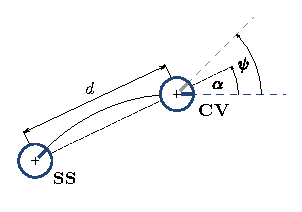
\includegraphics[width=0.5\textwidth]{media/robot_relative_movement.pdf}
 \end{center}
 \caption{Description of the motion parameters $d, \alpha, \psi$. The two circles depict the robot position and orientation (blue angle marks) under which the snapshot $\img{SS}$ and current view $\img{CV}$ were captured. The actual robot trajectory (solid line) is not required as the motion is fully described by the translatory distance $d$, the movement direction $\alpha$ and the change in orientation expressed by $\psi$.}
 \label{fig:robot_relative_movement}
\end{figure}

\begin{figure}[tbp]
  \begin{center}
   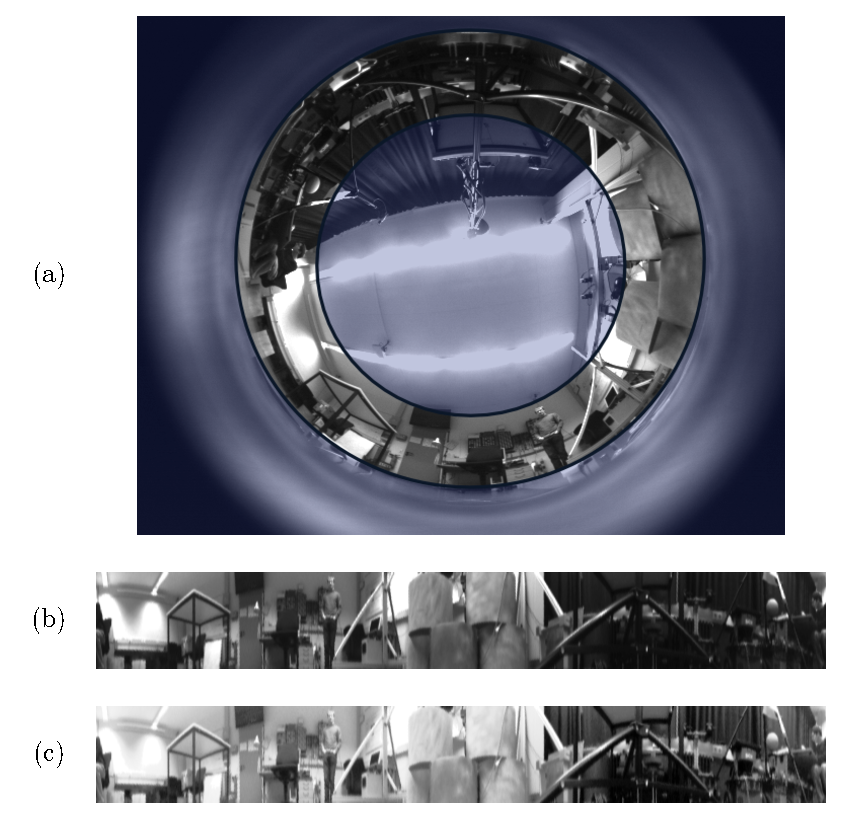
\includegraphics[scale=0.65]{media/cylindrical_panoramic_images_unprojected_pix.pdf}
  \end{center}
  \caption{(a) The original $640 \times 512$ pixel frame as recorded by the camera. The region used for the panoramic image is highlighted, with the outer circle being the bottom row in the result images (specified by the \textit{depression} angle $\check \gamma$) and the inner circle being the top row in the result images (specified by the \textit{elevation} angle $\hat \gamma$). (b) The unrolled $720 \times 96$ pixel cylindrical panoramic image. (c) Cylindrical image after applying histogram equalization.}
  \label{fig:cylindrical_panoramic_images_unprojected}
\end{figure}

The input of the obstacle detection algorithm is given as a pair of monochrome panoramic images, denoted $\img{SS}$ and $\img{CV}$ (snapshot and current view), accompanied by a set of motion parameters $d, \alpha$ and $\psi$.

\paragraph{Motion parameters:} As depicted in figure \ref{fig:robot_relative_movement} the motion parameters $d, \alpha$ and $\psi$ describe a motion vector leading from the snapshot position to the current view position. The Euclidean distance in meters is denoted by $d$, whereas the motion direction is denoted by the angle $\alpha$. The change in orientation under which the two images were captured is denoted by $\psi$.

\paragraph{Panoramic images:}
\label{sec:panoramic_image}
The fisheye images as captured from the camera are not directly used in the algorithm. As discussed in the introduction (section \ref{sec:intro_special}), the actual region of interest is too small to justify the usage of the complete input image. Instead the interesting region is mapped (using a lookup table that is generated in a calibration process) to a spherical panoramic image. The source region is chosen larger than the region of interest, as this extension will later (see section \ref{sec:memory_layout}) be needed for pixel lookups. Additionally, histogram equalization is applied to the images in order to increase the contrast and to compensate global illumination changes. See figure \ref{fig:cylindrical_panoramic_images_unprojected} for an example. This and the following chapters assume such a spherical panoramic image and are independent of the actual image source.

\paragraph{Panoramic image coordinate system:}
\label{sec:panoramic_coordinates}
The panoramic images contain a $360^\circ$ view of the surroundings such that the $x$-, $y$-pixel coordinates of the image linearly correspond to a pair of angles $\beta, \gamma$ which --- in conjunction with the yet unknown landmark distance $r$ --- describe the position of the projected landmark in spherical coordinates (note that an elevation angle of $\gamma = 0$ corresponds to the image horizon and not the zenith). Let $w, h$ denote the image width and height. It holds:
\begin{align*}
 \beta(x) &= \frac{2 \pi}w \cdot x & \gamma(y) &= \frac{\check \gamma - \hat \gamma}{h - 1} \cdot y + \hat \gamma
\end{align*}
where $\check \gamma$ is the so called \textit{depression} describing the elevation angle of the bottom image row and $\hat \gamma$ the so called \textit{elevation} describing the elevation angle of the top image row. The angles $\beta$ and $\gamma$ respectively correspond to azimuthal component and polar component of spherical coordinates (see figure \ref{fig:cylinder_coordinates_simple} for an illustration).

In contrast to classical spherical coordinates, the distance $r = \tilde r \cdot \cos(\gamma)$ (with $\tilde r$ being the Euclidean distance) is measured as ground distance, which will allow for simplified equations and the separability of the motion field equation, as discussed in section \ref{sec:flow_template_calculation}. As depicted in figure \ref{fig:hypot_vs_ground_distance}, the change in the measurement of $r$ only effects the representation of a series of equal-distanced landmarks. Moreover, points with an elevation angle of $\gamma = \pm 90^\circ$ cannot be uniquely described in this coordinate system.

Because $\beta, \gamma$ and the pixel coordinates $x, y$ can be used synonymously, the individual intensity values of an image $\img{I}$\footnote{A note on notation: Two-dimensional fields $\img{I}$ of scalars or low dimensional vectors (images, depth maps, index maps) are denoted in bold letters. This is not true for ``small'' matrices (convolution kernels), fields of functions or fields of sets.} are subsequently denoted by $\img{I}(\vec p) = \img{I}(\beta, \gamma)$. As the panoramic images are cyclic in horizontal direction, arbitrary $\beta$ values are cyclically mapped onto the interval $[0, 2\pi)$. If the pixel coordinates $x, y$ corresponding to a $\beta, \gamma$ pair are non-integral, bilinear interpolation between the neighboring pixels is applied.

\begin{figure}[p]
  \begin{center}
   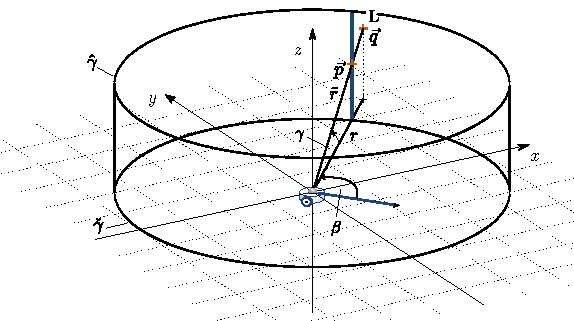
\includegraphics[width=0.975\textwidth]{media/cylinder_coordinates_simple.pdf}
  \end{center}
  \caption{Spherical coordinate system used throughout the algorithm. The projected position $\vec p$ of the landmark $L$ is given by the azimuthal angle $\beta$ and the elevation angle $\gamma$. The landmark position is given by $\beta, \gamma$ and the ground distance $r$.}
  \label{fig:cylinder_coordinates_simple}
\end{figure}

\begin{figure}[p]
  \begin{center}
   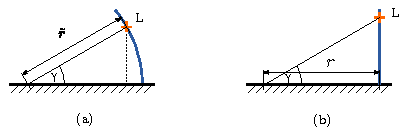
\includegraphics[width=0.8\textwidth]{media/hypot_vs_ground_distance.pdf}
  \end{center}
  \caption{Comparison between classical spherical coordinates (a) and the modified spherical coordinates (b). In (a), $\tilde r$ is measured as the distance between the coordinate-system origin and the landmark point $L$ (corresponds to the length of the hypotenuse in the above triangle). Landmarks with the same distance $\tilde r$ are thus assumed to be curved towards the camera (blue line). In the modified spherical coordinates depicted in (b), the distance $r$ is measured as the ground distance to the landmark. Consequently landmarks with the same distance $r$ shape a straight vertical line. As a side-effect, the elevation angle $\gamma$ is not of interest when a landmark point is $\vec q$ projected onto the $x$-$y$-plane. In contrast to classical spherical coordinates, points with $\gamma = \pm 90^\circ$ and $r = 0$ cannot be uniquely described in the modified spherical coordinates.}
  \label{fig:hypot_vs_ground_distance}
\end{figure}

\subsection{Assumptions}

\label{sec:assumptions}

The algorithm contains several idealizing assumptions, which may not be fully valid in a real-world environment. These assumptions cover both the robot and its environment.
\begin{enumerate}[(1)]
 \item \textit{Perfect path integration:} The robot is capable of perfect path integration and can thus (given an initial offset) determine its current world position and orientation at any time step. There is no mobile robot which completely fulfills this assertion without an external position reference \citep[chapter 3, ``Mobile Robot Kinematics'', p. 57ff]{AutonomousMobileRobots}. Yet the relative movement measured by the odometry over a short time window (as needed in the algorithm) and in ``normal'' operation (no wheel slippage) is assumed to be relatively error-free.
 \item \textit{Limited degrees of freedom:} It is assumed that the robot is only moving in the $x$-$y$-plane and only rotates around its $z$-axis. Neither is there any change in the elevation, nor does the robot tilt around any other axis. Those assumptions are likely to be violated in the real-world. Especially in outdoor environments the ground is never perfectly even and thus both changes in elevation and tilt can occur. In indoor environments e.g. carpets or thresholds are possible problems. We may assume that any tilting is removed from the input images in a preprocessing step, yet this is out of the scope of this thesis.
 \item \textit{Brightness constancy:} Neither are there changes in the global illumination (e.g. lights being switched on/off or the sun being covered by clouds) nor does the surface brightness change between the images. As pointed out by \cite{flowchapter05}, this ``brightness constancy'' only holds in environments containing surfaces without specularities (Lambertian surfaces), ``a distant point light source, no object rotations and no secondary illumination (shadows or inter-surface reflection)''. Yet this brightness constancy assumption (especially the lack of specularities) is used in most optical flow algorithms and seems to work remarkably well in practice.
 \item \textit{Static world:} The world is static, the robot is the only moving entity. This assumption may not be fulfilled in outdoor environments with vegetation and also in crowded indoor scenes. Moving objects may cause wrong depth reconstruction and thus cause false positive obstacles. Therefore the navigation algorithm which processes the obstacle points returned by the algorithm must be capable of discarding obstacles in its internal map that prove to be nonexistent.
\end{enumerate}
The robustness of the algorithm regarding violation of assumption (1) is explicitly tested in section \ref{sec:noise}.

\section{Depth reconstruction}

\label{sec:outline}

The goal of the \textit{depth reconstruction} stage is to estimate the ground distance $r$ for the landmarks corresponding to each pixel $\vec p = (\beta, \gamma)^T$ in the current view image $\img{CV}$. Consequently, the required result is a depth map $\img{R}(\vec p)$.

The general idea of the depth reconstruction is to exploit the parallax information present in the two images: Objects with a large distance only show a small displacement between the two images, whereas objects close to the camera show a relatively large displacement. This object displacement information is described by the motion field.

First a short introduction to optical flow estimation will be given. In conjunction with the motion parameters, the minimization problem underlying optical flow can then be reduced from a two-dimensional problem in each image point to a one dimensional problem. An approximative heuristic for this one dimensional problem is then given as minimum search in the so called \textit{error stack}.

\subsection{Short introduction to optical flow estimation}

When moving a camera in a static 3D-scene, the projected object points move along certain two-dimensional paths. These paths depend on the camera motion, the object distance and position in the projected image. The velocity of each pixel at position $x, y$ in the image and time $t$ is referred to as \textit{motion field} \citep{flowchapter05}. The motion field is a theoretical construct which can only be calculated if the camera parameters, camera motion and the exact position of each landmark point $\vec q$ are known.

Optical flow is an estimation of the motion field for a set of images $\img{I}_1$ and $\img{I}_2$ captured at discrete times $t_1$ and $t_2$ during the camera movement (in general optical flow may be estimated from more than two images). By definition, optical flow cannot express the motion of the underlying objects, but of the light intensities created by these objects \citep[][chapter 4.2.7 ``Motion and optical flow'', p. 189]{AutonomousMobileRobots}. The global optical flow estimation problem can generally be expressed as finding a vector field $\vec u : \R^2 \longrightarrow \R^2$ which minimizes the following error function \citep[adapted from][]{hornSchunck}:
\begin{equation}
  E(\vec u) = \int_{\vec p} \left( \|\img{I}_1(\vec p) - \img{I}_2(\vec p + \vec u(\vec p))\|_1 + \lambda \| \nabla \vec u(\vec p) \| \right) \; \mathrm{d}\vec p \label{eqn:optical_flow} \; .
\end{equation}
The first summand $\|\img{I}_1(\vec p) - \img{I}_2(\vec p + \vec u(\vec p))\|$ expresses the residual error after warping the second image according to the vector field. Note that minimization of this term is only valid due to assumptions (3) (brightness constancy) and (4) (static world).

The second term $\lambda \| \nabla \vec u(\vec p) \|$  enforces a certain ``smoothness'' to the vector field under the regularization parameter $\lambda$. This regularization is crucial for eliminating trivial solutions, such as simply mapping pixels with the same intensity to each other.

Although some approaches try to globally solve the minimization problem stated by equation \ref{eqn:optical_flow} \citep[e.g.][chapter 5 ``Real-time Optical Flow'']{totalVariation}, the solution presented here only minimizes the error for the local surroundings of each pixel in order to fulfill the real-time constraint on an embedded system.

\subsection{Motion field equation}

Given the motion parameters $d, \alpha, \psi$, the motion field could actually be calculated if the distance to each landmark point $\img{R}(\vec p)$ was known:

Let $\vec q = (x, y, z)^T$ be the position of a landmark $L$ in robot coordinates (origin at the robot center, $x$-axis aligned with the robot orientation). The projection $P : \R^3 \longrightarrow \R^2 $ that projects $\vec q$ onto $\vec p = (\beta, \gamma)^T$ in the image plane is given as:
\begin{equation}
 \vec p = P(\vec q) = \begmat \beta \\ \gamma \finmat = \begmat
  \atantwo(y, x) \\
  \arctan\left(\frac{z}{\sqrt{x^2 + y^2}}\right)
 \finmat
 \label{eqn:project}
\end{equation}
The inverse $P^{-1} : \R^2 \longrightarrow \R^3$ with free parameter $r$ (ground distance) is given as:
\begin{equation}
 \vec q = P^{-1}(\vec p; r) = \begmat x \\ y \\ z \finmat = r \cdot \begmat
  \cos(\beta) \\
  \sin(\beta) \\
  \tan(\gamma)
 \finmat
 \label{eqn:unproject}
\end{equation}
The motion vector $\vec u(\vec p; T, r)$ describing the relative movement of a pixel at position $\vec p$ between the current view and the snapshot image can now be calculated as
\begin{equation}
 \vec u(\vec p; T, r) = P(T \cdot h(P^{-1}(\vec p; r))) - \vec p \label{eqn:motion_field_vector}
\end{equation}
where $T \in \R^{3 \times 4}$ is a homogeneous transformation matrix expressing the robot movement between $\img{CV}$ and $\img{SS}$ in world coordinates:
\begin{equation}
 T = T(d, \alpha, \psi) = \begmat
   \cos(\psi) & \sin(\psi) & 0 & d \cdot \cos(\alpha) \\
  -\sin(\psi) & \cos(\psi) & 0 & d \cdot \sin(\alpha) \\
 0 & 0 & 1 & 0
 \finmat
 \label{eqn:transform}
\end{equation}
The sole purpose of the mapping $h : \R^3 \longrightarrow \R^4$ is to transform three dimensional points to homogeneous coordinates. $h$ is defined as $(x, y, z)^T \mapsto (x, y, z, 1)^T$. See figure \ref{fig:cylinder_coordinates_transformation} for an interpretation of the motion field vectors.

\begin{figure}[t]
 \begin{center}
  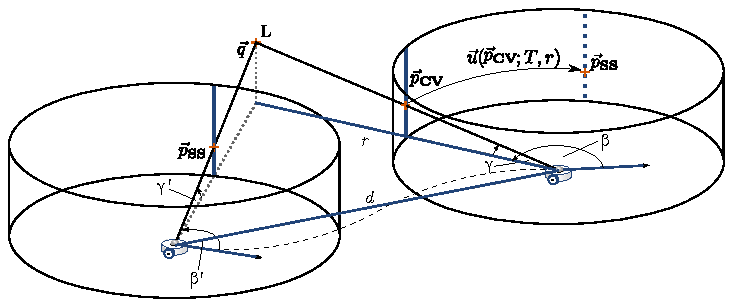
\includegraphics[width=0.975\textwidth]{media/cylinder_coordinates_transformation.pdf}
 \end{center}
 \caption{The motion field equation can be interpreted as follows: Given a point $\vec p_{\img{CV}} = (\beta, \gamma)^T$ in $\img{CV}$ (right), the motion field vector $\vec u(\vec p_{\img{CV}}; T, r)$ predicts the position $\vec p_{\img{SS}} = (\beta', \gamma') = \vec u(\vec p_{\img{CV}}; T, r) + \vec p_{\img{CV}}$ in which the same landmark point $L$ would be visible in $\img{SS}$ (right) under the assumption that $L$ has the distance $r$.
}
 \label{fig:cylinder_coordinates_transformation}
\end{figure}

\subsection{Flow parametrization}

By combining equation \ref{eqn:motion_field_vector} from above and the error function in equation \ref{eqn:optical_flow}, the minimum search can be reduced from a two-dimensional problem in each pixel (finding an arbitrary flow vector $\vec u$) to a one dimensional optimization problem (finding the best matching depth value $r$ for each pixel):
\begin{equation}
 E(\img{R}) = \int_{\vec p} \left( \|\img{I}_1(\vec p) - \img{I}_2(\vec p + \vec u(\vec p;  T, \img{R}(\vec p)))\|_1 + \lambda \nabla \| \vec u(\vec p; T, \img{R}(\vec p)) \| \right) \;\mathrm{d}\vec p\label{eqn:parametrized_optical_flow}
\end{equation}
Hence the depth field $\img{R}(\vec p)$ can be seen as an implicit characterization of the optical flow field under the motion parameters $d, \alpha$ and $\psi$. Note that these parameters are only known if assumption (1) (perfect path integration, see section \ref{sec:assumptions}) is valid --- otherwise the motion field cannot be predicted.

\subsection{Error stack calculation}

\label{sec:error_stack}

The heuristic used in this approach searches local minima in the so called \textit{error stack} $\img{E}$ in order to estimate the depth field $\img{R}(\vec p)$. Each of the $n$ layers $\img{E}_i$ contains the residual error (first summand in equation \ref{eqn:parametrized_optical_flow}) evaluated for a constant depth $r_i$:
\begin{equation}
 \img{E}_i(\vec p) = \|\img{CV}(\vec p) - \img{SS}(\vec p + \vec u(\vec p; T, r_i))\|_1 \text{ where }  0 \leq i < n \label{eqn:error_stack_layer}
\end{equation}
Figuratively speaking, this equation is equivalent to first calculating a warped snapshot image $\img{SS'}_i$, that predicts ``what the current view would look like'' under the assumption that all image points had the same distance $r_i$. The residual error stored in each error stack layer is then given as $\img{E}_i = \| \img{CV} - \img{SS'}_i \|_1$. See figure \ref{fig:error_stack} for an example.

Note that some source pixel coordinates may not be in range when calculating the warped snapshot. The error value stored for the target pixel in the error stack layer should then be set to a large value (see figure \ref{fig:error_stack}).

\paragraph{Conventions for the distance series:} The $r_i$ are left open at this point, yet (by convention) any choice has to meet the following conditions:
\begin{enumerate}[1.]
 \item The series $r_i$ is strictly monotonically decreasing.
 \item $r_0 = \infty$ (for $i = 0$ the motion vector length should equal zero for all pixels).
 \item The step from $r_i$ to $r_{i + 1}$ should increase the maximum horizontal flow vector length by one pixel. This way the pixels in $\img{SS'}_i$ are at most shifted by one pixel in horizontal direction between two error stack layers, which allows to exploit the complete horizontal image resolution in the error stack calculation.
 \item $r_{n - 1}$ should be chosen near the smallest possible distance between an obstacle and the camera.
 \item There has to be some strictly monotonically decreasing, continuous function $r(j) : \R^+ \longrightarrow \R^+$, where $r(i) = r_i$ for all $i$.
\end{enumerate}
A concrete choice for the $r_i$ is presented in section \ref{sec:index_to_depth}.

\paragraph{Index related error function:} Combining the error stack equation (\ref{eqn:error_stack_layer}) and the parametrized optical flow equation (\ref{eqn:parametrized_optical_flow}) yields a minimization of the \textit{index field} $\img{J}(\vec p)$, that describes the error stack index chosen for each pixel:
\begin{align}
 E(\img{J}) &= \int_{\vec p} \left( \img{E}_{\img{J}(\vec p)}(\vec p) + \lambda \| \nabla \vec u(\vec p; T, r(\img{J}(\vec p))) \| \right) \; \mathrm{d}\vec p \nonumber \\
 &\approx \int_{\vec p} \left( \img{E}_{\img{J}(\vec p)}(\vec p) + \lambda \| \nabla \img{J}(\vec p) \| \right) \; \mathrm{d}\vec p \label{eqn:global_min_index}
\end{align}

At first glance $\nabla \vec u(\vec p; T, r({\img{J}(\vec p))}) \approx \nabla \img{J}(\vec p)$ seems to be a very rough approximation, yet due to the conventions presented above, the error stack index $i$ is approximately proportional to the flow vector length. Consequently a smooth index field $\img{J}(\vec p)$ implies a smooth flow vector field $\vec u(\vec p; T, r({\img{J}(\vec p))})$.

\begin{figure}[p]
 \centering
 \begin{footnotesize}
 \begin{tabular}{m{0.025\textwidth} m{0.575\textwidth} m{0.4\textwidth}}
  (a) & 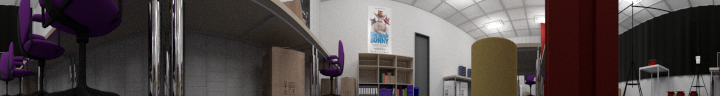
\includegraphics[width=0.55\textwidth]{media/warped/cv.png} & $\img{CV}$ (current view image) \\
  (b) & 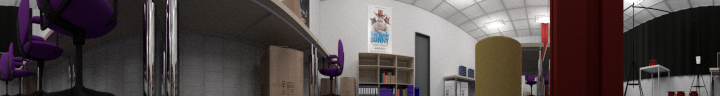
\includegraphics[width=0.55\textwidth]{media/warped/ss.png} & $\img{SS}$ (snapshot image) \\
  (c) & 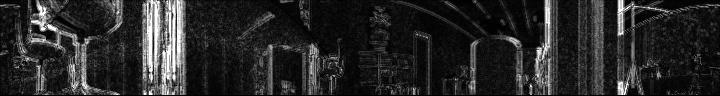
\includegraphics[width=0.55\textwidth]{media/warped/warped_depth_0.png} & $\img{E}_1$ with $r_1 = \infty$ \\
  (d) & 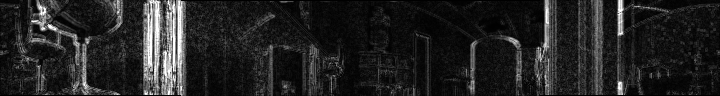
\includegraphics[width=0.55\textwidth]{media/warped/warped_depth_1.png} & $\img{E}_2$ with $r_2 = 4.58 \, \mathrm{m}$ \\
  (e) & 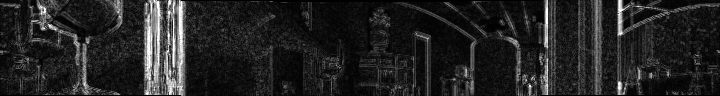
\includegraphics[width=0.55\textwidth]{media/warped/warped_depth_2.png} & $\img{E}_3$ with $r_3 = 2.29 \, \mathrm{m}$ \\
  (f) & 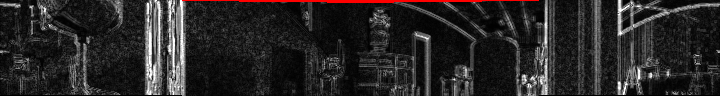
\includegraphics[width=0.55\textwidth]{media/warped/warped_depth_3.png} & $\img{E}_4$ with $r_4 = 1.15 \, \mathrm{m}$ \\
  (g) & 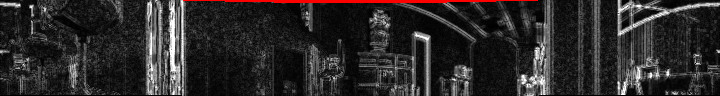
\includegraphics[width=0.55\textwidth]{media/warped/warped_depth_4.png} & $\img{E}_5$ with $r_5 = 0.92 \, \mathrm{m}$ \\
  (h) & 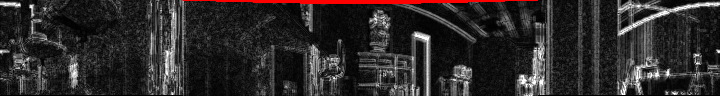
\includegraphics[width=0.55\textwidth]{media/warped/warped_depth_5.png} & $\img{E}_6$ with $r_6 = 0.76 \, \mathrm{m}$ \\
  (i) & 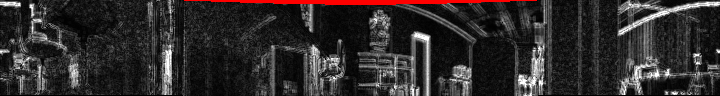
\includegraphics[width=0.55\textwidth]{media/warped/warped_depth_6.png} & $\img{E}_{15}$ with $r_{15} = 0.31 \, \mathrm{m}$
 \end{tabular}
 \end{footnotesize}
 \caption{Visualization of a series of error stack layers. The error stack layers shown in the images (c) to (i) were calculated for the current view and snapshot shown in (a) and (b) (the original input images are monochrome). The brightness of the pixels in the error stack images corresponds to the error value. Note how certain objects ``disappear'' (have only a small error) in certain error stack images, like the silhouettes of the yellow cylinder in $\img{E}_5$ or the table legs in $\img{E}_6$, while the error for distant objects like the door frame increases with each layer. The image regions marked red form those for which no prediction can be made and thus have an infinite error.}
 \label{fig:error_stack}
\end{figure}

\subsection{Input image augmentation}

\label{sec:preprocessing}

\begin{figure}[p]
	\centering
	\subbottom[Monochrome image]{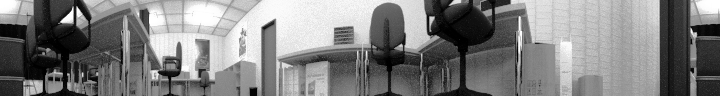
\includegraphics[width=0.75\textwidth]{media/gradient/in_brightness.png}}
%	\subbottom[$x$-derivative]{\includegraphics[scale=0.248]{media/gradient/in_derivative_x.png}}
%	\subbottom[$y$-derivative]{\includegraphics[scale=0.248]{media/gradient/in_derivative_y.png}} \\
	\subbottom[Combined pseudocolor image]{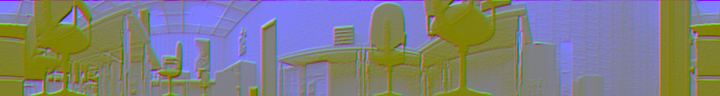
\includegraphics[width=0.75\textwidth]{media/gradient/out.png}}
	\caption{Comparison between the original monochrome image and the pseudo-color image resulting from the transformation described in equation \ref{eqn:dimensionality_increase}. The brightness is mapped to the blue channel, $x$- and $y$-derivatives to the red and green channels, respectively.}
	\label{fig:pseudocolor_image}
\end{figure}

Comparing individual pixels from a monochrome image $\img{I}$ (as in the error stack equation \ref{eqn:error_stack_layer}) discards all spatial information that is encoded in the environment of each pixel.

In order to increase the information contained within a single pixel, one can increase its dimensionality. In the resulting feature space, each pixel can be seen as a local feature descriptor. The augmentation proposed here adds the image gradients in horizontal and vertical direction as a second and third component to each pixel, leading to the following equation for the augmented image $\img{\tilde I}$:
\begin{equation}
	\img{\tilde I}(\vec p) = \begmat
		\img{I}(\vec p),
		\left. \frac{\partial \img{I}}{\partial x \vphantom{y}} \right|_{\vec p},
		\left. \frac{\partial \img{I}}{\partial y} \right|_{\vec p}
	\finmat^T
	\label{eqn:dimensionality_increase}
\end{equation}
As a drawback, this augmentation reduces the overall spatial resolution: Estimating the derivative on discrete images (e.g. using the $3 \times 3$ Sobel kernel) incorporates at least three pixels. Moreover, the derivation increases the image noise \citep[][p. 200]{AutonomousMobileRobots}.

Figure \ref{fig:pseudocolor_image} shows the result of equation \ref{eqn:dimensionality_increase} being applied to an input image. Note how the image edges (representing the regions with the largest gradient) are prominently marked in the resulting image. Thus ``a sense of edges'' is added to the algorithm.

\subsection{Minimum error search}

\label{sec:minimum_error_search}
As stated in equation \ref{eqn:global_min_index}, estimating depth and optical flow is a matter of minimizing the global error by choosing appropriate error stack indices $\img{J}(\vec p)$ for each pixel $\vec p$. A na\"{\i}ve heuristic to estimating depth for each pixel would be to simply select the error stack layer that holds the global minimum error for each pixel:
\begin{equation}
	\img{J}(\vec p) = \arg \min_{i} \img{E}_i(\vec p) \label{eqn:naive_minimum_search}
\end{equation}
However, while being very simple to compute, this heuristic has a severe disadvantage: Computing the index without regarding neighboring pixels completely disregards the smoothness term. Additionally, as the error stack may not have a single pronounced minimum but multiple local minima with very small difference, the result is prone to noise.

Assuming that most objects cover more than a single pixel in the image and neighboring pixels have approximately the same distance, we can modify equation $\ref{eqn:naive_minimum_search}$ to respect the surroundings of each pixel. Let $W_{\vec p}$ be a (possibly space-variant) two-dimensional filter kernel with radius $r_W$:
\begin{equation}
	\img{J}(\vec p) = \arg \min_{i} \left( \img{E}_i \ast W_{\vec p} \right)_{\vec p} \label{eqn:kernel_minimum_search}
\end{equation}
The matrix $W_{\vec p}$ is subsequently called \textit{error propagation matrix} as it ``propagates'' error values from neighboring pixels to its center pixel.

In large homogeneous image regions where multiple error stack layers contain very small error values (see the wall regions in figure \ref{fig:error_stack}), depth cannot be reconstructed (at least not without using global approaches) and equation \ref{eqn:kernel_minimum_search} will very likely produce noise in such regions. In a later step, this noise might produce unwanted false obstacle points. Adding a linear bias $\tau \cdot i$ to the error function allows to classify homogeneous image regions  as ``very distant'', in which case they do not hinder the obstacle detection:
\begin{equation}
	\img{J}(\vec p) = \arg \min_{i} \left( \left( \img{E}_i \ast W_{\vec p} \right)_{\vec p} + \tau \cdot i \right) \label{eqn:kernel_minimum_search_bias}
\end{equation}

\paragraph{Choices for $W_{\vec p}$:} Simple space-invariant choices for $W_{\vec p} = W$ include a matrix of ones or a Gaussian filter kernel. A space-variant filter kernel $W_{\vec p}$ which takes object boundaries into account and thus only propagates error values for pixels belonging to the same object is presented in appendix \ref{sec:kernels}.

\subsection{Minimum error refinement}

\label{sec:index_field_refinement}

\begin{figure}[t]
 \begin{center}
  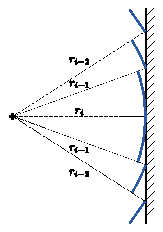
\includegraphics[width=0.35\textwidth]{media/discrete_indices_artifacts.pdf}
 \end{center}
 \caption{Local map (top-down view) showing the artifacts created by approximating a planar surface with a set of circles having discrete radii (blue).}
 \label{fig:discrete_indices_artifacts}
\end{figure}

% \begin{figure}[p]
%  \begin{center}
%    \includegraphics[width=0.975\textwidth]{media/minimum_error_search.pdf}
%   \end{center}
%   \caption{Visualization of the minimum error search in the error stack layers. For each pixel $\vec p$ the minimum error is searched within a region specified by the filter kernel $W_{\vec p}$. The discrete minimum index $\img{J}(\vec p)$ is then refined by searching the minimum $\img{\tilde J}(\vec p)$ in the piecewise error stack approximations plus a regularization term. The piecewise error stack approximations are indicated by the dashed blue lines in the image.}
%   \label{fig:minimum_error_search}
% \end{figure}

Equation $\ref{eqn:kernel_minimum_search}$ produces an index field $\img{J}(\vec p)$ consisting of discrete values. This is especially problematic if a planar surface needs to be reconstructed (see figure \ref{fig:discrete_indices_artifacts}). Additionally, the discontinuity causes a high penalty in the smoothness term of the global error equation \ref{eqn:optical_flow}. In this section the initial index field $\img{J}(\vec p)$ as defined in equation $\ref{eqn:kernel_minimum_search_bias}$ will be refined (allowing non-discrete solutions) and regularized (addressing the smoothness term) which leads to the final index field $\img{\tilde J}(\vec p)$.

\paragraph{Refinement:} The discontinuity problem can be solved by approximating the error stack in each layer $i$ and pixel $\vec p$ utilizing piecewise polynomials of second degree (quadratic; allows for trivial analytical solution), resulting in a set of functions $\tilde E_{i}(j; \vec p)$ with the following properties:
\begin{equation*}
	\begin{aligned}
		\tilde E_{i}(j; \vec p) &:= \begmat j^2 & j & 1 \finmat \cdot \vec w \\
		\tilde E_{i}(i + j; \vec p) &\overset{!}= \img{E}_{i + j}(\vec p) + \tau \cdot (i + j)\quad \forall \quad j \in \{-1, 0, 1\}
	\end{aligned}
\end{equation*}
Solving this set of linear equations yields the following weight vector $\vec w$:
\begin{equation}
	\vec w = \begmat w_2 \\ w_1 \\ w_0 \finmat =
	\begmat
		\frac{1}2 & -1 & \frac{1}2 \\
		-i - \frac{1}2 & 2 i & -i + \frac{1}2 \\
		\frac{1}2(i^2 + i) & -i^2 + 1 & \frac{1}2 (i^2 - i)
	\finmat
	\cdot
	\begmat
		\mathbf{E}_{i - 1}(\vec p) + \tau \cdot (i - 1) \\
		\mathbf{E}_{i}(\vec p) + \tau \cdot i \\
		\mathbf{E}_{i + 1}(\vec p) + \tau \cdot (i + 1)
	\finmat
	\label{eqn:polynomial_coeffs}
\end{equation}
If one of the error layers $\mathbf{E}_{i - 1}$ or $\mathbf{E}_{i + 1}$ does not exist, a linear approximation is chosen instead.

\paragraph{Regularization:} The regularization term penalizes large variances in the index field. For a single reference point $\vec q$, the quadratic regularization function $R(j; \vec q)$ is given as a polynomial
  $$R(j; \vec q) = \lambda \cdot (\img{J}(\vec q) - j)^2$$
which quadratically increases the penalty according to the difference between the index $j$ in the current point $\vec p$ and the index of the reference point $\vec q$.

\paragraph{Final minimization formula:} Again the error function is not minimized for every individual pixel, but for a weighted region surrounding each pixel as defined by the convolution kernel $W_{\vec p}$. For compact notation, let $A(\vec p) := \{\vec p + (\beta(x), \gamma(y))^T \mid -m \leq x, y \leq m\}$ denote the pixel coordinates beneath the convolution window at position $\vec p$ and let $\omega_{\vec p}^{\vec q}$ for $\vec q \in A(\vec p)$ denote the corresponding value in the convolution matrix $W_{\vec p}$. The refinement of the initial (integral) index field $\img{J}$, leading to the refined, real-valued index field $\img{\tilde J}$, is then given as
\begin{equation}
 \img{\tilde J}(\vec p) = \argmin_{\img{J}(\vec p) - 1 \leq j \leq \img{J}(\vec p) + 1} \sum_{\vec q \in A(\vec p)} \omega_{\vec p}^{\vec q} \cdot \left(\tilde E_{\img{J}(\vec p)}(j; \vec q) + R(j; \vec q) \right)
 \label{eqn:index_field_refinement}
\end{equation}
As the sum only contains quadratic polynomials, the minimum can be calculated analytically.

Note that the refinement step can be repeated multiple times. The indices in $\img{\tilde J}(\vec p)$ are then rounded to the nearest integers and treated as the initial index field $\img{J}(\vec p)$.

Once the final index map $\img{\tilde J}(\vec p)$ has been built, the index-to-depth function $r(j)$ can be used to obtain the desired depth map:
  $$\img{R}(\vec p) = r(\img{\tilde J}(\vec p))$$


\section{Obstacle detection}

The simple heuristic used in the depth reconstruction was designed for fast evaluation and does by no means guarantee to find a perfect depth estimation. Additionally, noise in the images or the motion parameters $d, \alpha, \psi$ (and thus a violation of the assumptions presented in section \ref{sec:assumptions}) inevitably leads to noise in the depth map.

For obstacle detection, a local environment map (top-down projection onto the $x$-$y$-plane) of the reconstructed landmark points is created. The aim of this map is to improve the depth reconstruction result by combining depth maps resulting from multiple depth reconstruction steps. It then allows the selection of actual obstacle points which form the result of the overall algorithm.

\subsection{Probabilistic landmark model}

\label{sec:prob_landmarks}

\begin{figure}[p]
 \begin{center}
  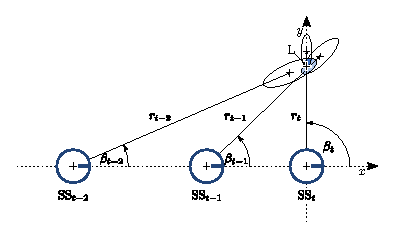
\includegraphics[width=0.82\textwidth]{media/obstacle_map_jitter.pdf}
 \end{center}
 \caption{The Gaussian distributions for reconstructed landmark positions from multiple time steps can overlap in such a way that their sum forms a distinct maximum at (or at least near) the actual landmark position $L$. Consequently, whenever a value above a certain threshold appears in the map, the underlying point is emitted as an obstacle. Note that the sum of two overlapping (corresponding to the intersection of certain contour lines) Gaussian distributions does not necessarily yield a maximum at the landmark position as suggested by the drawing. Yet the distributions used in this approach have a relatively high distance variance $\sigma_r$ in comparison to their direction variance $\sigma_\beta$. Thus overlapping Gaussians implicitly triangulate the landmark and a maximum is probable.}
 \label{fig:obstacle_map_jitter}
\end{figure}

\begin{figure}[p]
 \begin{center}
  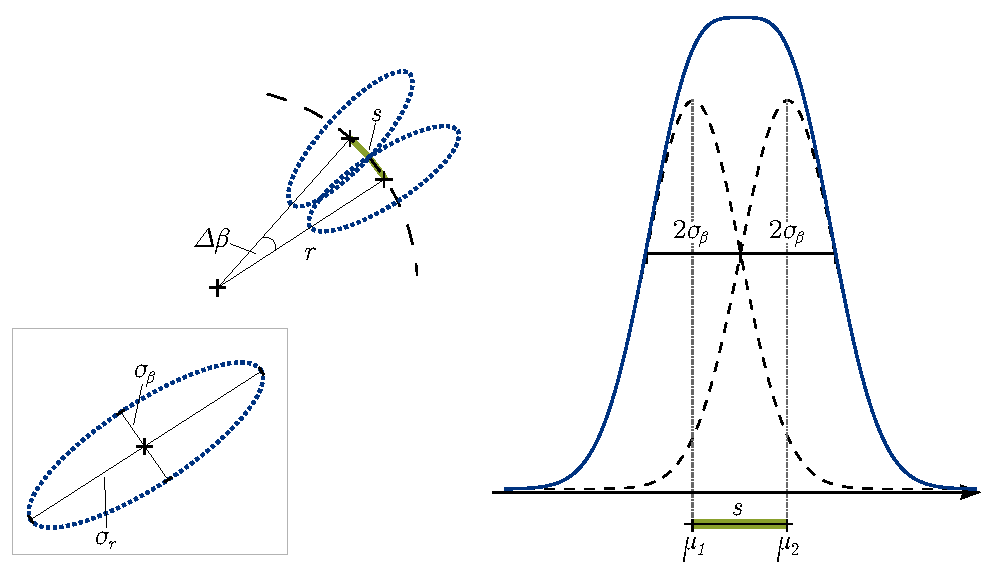
\includegraphics[width=0.91\textwidth]{media/sigma_beta.pdf}
 \end{center}
 \caption{Calculation of the variance $\sigma_\beta$. Adjacent Gaussian distributions with the same radius $r$ should form a nearly uniform distribution between $\mu_1$ and $\mu_2$. See also appendix \ref{proof:sigma_beta}.}
 \label{fig:sigma_beta}
\end{figure}

The reconstructed landmark points $(\beta, \gamma, r)^T$ can be projected onto the $x$-$y$-plane by just omitting the $\gamma$ angle, as $r$ was chosen as the ground distance (see section \ref{sec:panoramic_coordinates} and the corresponding figure \ref{fig:hypot_vs_ground_distance}). The projected landmark point $\vec q$ is hence specified by the polar coordinates $\vec q = (\beta, r)^T$.

As stated above, the \textit{estimated} landmark position $\vec q_E$ as returned from the depth reconstruction is prone to noise. Assume a Gaussian distribution with mean at $\vec q_E$ for the probability of the \textit{real} landmark position $\vec q_R$:
\begin{equation}
  \vec q_R \sim \mathcal{N}\left(\vec q_E, \Sigma(\vec q_E) \right) \text{ where } \Sigma(\beta, r) := \begmat \sigma_\beta^2 & 0 \\ 0 & \sigma_r^2 \finmat
  \label{eqn:gaussian_polar}
\end{equation}
Let $\mathcal{C} : (\beta, r)^T \mapsto r \cdot (\cos(\beta), \sin(\beta))^T$ denote the transformation from polar to Cartesian coordinates. As an approximation, equation \ref{eqn:gaussian_polar} can be written for Cartesian coordinates as:
\begin{equation}
  \mathcal{C}(\vec q_R) \sim \mathcal{N}\left(\mathcal{C}(\vec q_E), \Sigma_{\mathcal{C}}(\vec q_E)\right)
\end{equation}
where $\Sigma_{\mathcal{C}}$ is the corresponding covariance matrix in Cartesian space given as (see \ref{proof:covariance_matrix_transformation} for the derivation):
\begin{equation}
  \Sigma_{\mathcal{C}}(\beta, r) = \begmat
    (\sigma_r \cos(\beta))^2 + (r \sigma_\beta \sin(\beta))^2 & \cos(\beta) \sin(\beta) (\sigma_r^2 - (r \sigma_\beta)^2) \\
    \cos(\beta) \sin(\beta) (\sigma_r^2 - (r \sigma_\beta)^2) & (\sigma_r \sin(\beta))^2 + (r \sigma_\beta \cos(\beta))^2
  \finmat
  \label{eqn:cartesian_covariance}
\end{equation}


\paragraph{Derivation of the distribution variances:} Until now the variances in  direction $\sigma_\beta$ and in distance $\sigma_r$ were left open.

The distance variance $\sigma_r$ depends on the choice of the yet unknown index-to-depth function $r(j)$ and will be introduced along with the concrete choice in section \ref{sec:index_to_depth}.

However, $\sigma_\beta$ only depends on the horizontal image resolution $\Delta \beta := \nicefrac{2\pi}w$ and can be derived by demanding that two adjacent Gaussian distributions (with $| \beta_1 - \beta_2 | = \Delta \beta$) should overlap in such a way that their sum forms a near-uniform distribution in the region between $\beta_1$ and $\beta_2$. This choice is motivated by the fact that the probability of an obstacle point being located somewhere between two image columns $\beta_1$ and $\beta_2$ is the same as the probability of an obstacle point being located exactly on a certain image column $\beta$.

One can show (see appendix \ref{proof:sigma_beta}) that $\sigma_\beta$ is now given as
\begin{equation}
 \sigma_\beta = \frac{\Delta \beta}2 = \frac{\pi}{w}
 \label{eqn:sigma_beta} \; .
\end{equation}
Multiplying $\sigma_\beta$ with $r$ produces the Cartesian equivalent of the angular variance, as $\Delta \beta \cdot r$ denotes the length $s$ of the curve segment between $\beta_1$ and $\beta_2$ (see figure \ref{fig:sigma_beta}).

\subsection{Distribution accumulation and obstacle detection}

\label{sec:obstacle_detection}

It is hoped that the accumulated Gaussian distributions (forming the so called \textit{density values}) resulting from subsequent depth reconstruction steps produce pronounced maxima at the real landmark positions. This is possible as the probability distributions have rather small variance in angular direction, but a relatively large variance in distance direction. Thus intersecting Gaussian distributions implicitly triangulate the result (see figure \ref{fig:obstacle_map_jitter}).

Let $\img{M}$ be a discrete Cartesian map matrix that spans a region of $2 \cdot r_M \times 2 \cdot r_M$ meters (where $r_M$ is radius of the map), and let the origin $\img{M}(0, 0)$ correspond to the center of the map matrix. The obstacle detection algorithm is given as follows:

\paragraph{Map position update:} Rotate and shift the map matrix such that the camera is always located at the map origin and the angle $\beta = 0$ is always relative to the current translatory motion direction $\alpha$.

\paragraph{Map decay:} In order to ensure the locality of the map, all old density values are multiplied with a decay factor $\delta$ depending on the translatory distance $d$:
\begin{equation}
 \img{M}(x, y) \gets \img{M}(x, y) \cdot \delta \; \forall \; x, y \text{ where } \delta = \exp(-\epsilon \cdot d) \; .
 \label{eqn:map_decay}
\end{equation}
The free parameter $\epsilon$ is used as a conversion factor between $d$ and $\delta$. This way old density values are gradually discarded from the map as the robot moves through the world.

\paragraph{Distribution accumulation:} For each reconstructed and projected landmark point $\vec q_k = (\beta_k, r_k) \in Q$ the corresponding probability distributions are accumulated and added to the old density values in the discrete map:
\begin{equation}
 \img{M}(x, y) \gets \img{M}(x, y) + \sum_{\vec q \in Q} \mathcal{N}\left((x, y)^T \mid \mathcal{C}(\vec q), \Sigma_{\mathcal{C}}(\vec q)  \right) \; \forall \; x, y
\end{equation}

\paragraph{Obstacle detection:}

\begin{figure}[t]
 \begin{center}
  \subbottom[Color coded local environment map]{
    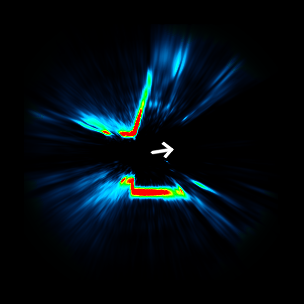
\includegraphics[width=0.3\textwidth]{media/local_obstacle_map_2.png}
  }
  \subbottom[Thresholded map]{
    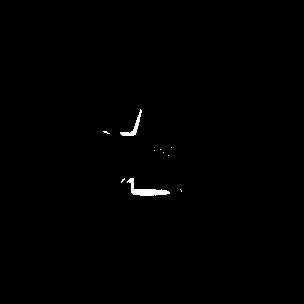
\includegraphics[width=0.3\textwidth]{media/local_obstacle_map_segmented.png}
  }
  \subbottom[Resulting obstacle points (orange)]{
    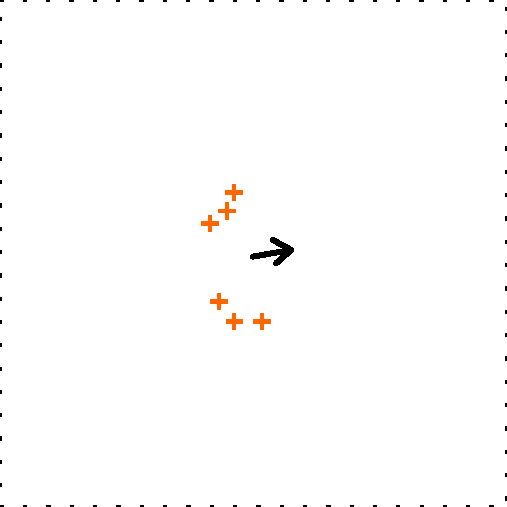
\includegraphics[width=0.3\textwidth]{media/local_obstacle_map_obstacles.pdf}
  }
 \end{center}
 \caption{Overview of the obstacle detection process. (a) shows a color coded environment map $\img{M}$ (black and blue correspond to small, green and yellow to medium and red to high density values), (b) shows the thresholded map $\img{\tilde M}$ and (c) the resulting obstacle points which form the result of the algorithm. The arrows in (a) and (c) indicate the robot orientation.}
 \label{fig:obstacle_map_process}
\end{figure}

If multiple distributions overlap in such a way that a distinct maximum is formed in the obstacle map, it is likely for this maximum to correspond to an actual landmark point. As outlined in figure \ref{fig:obstacle_map_process}, these distinct maxima are detected by generating a thresholded map
  $$\img{\tilde M}(x, y) \gets \begin{cases}
                              1 & \img{M}(x, y) > \eta \\
                              0 & \text{otherwise}
                             \end{cases} \quad \forall \; x, y$$
where $\eta$ is the threshold value. In a subsequent step, 4-connected components in $\img{\tilde M}$ are detected \citep[using the one-pass algorithm presented in][]{wiki:connected_component}. If they exceed a certain minimum size their centroid is returned as an obstacle point.

\paragraph{Obstacle point fragmentation and occupancy map:} As an extension to the above, large connected components are fragmented into multiple obstacle points. This is accomplished by dividing each connected component into square grid cells, counting the pixels in each cell and --- if a threshold is exceeded --- returning the centroid of the pixels in each grid cell as an obstacle point.

In order to prevent the algorithm from repeatedly returning the same obstacle points, obstacles are marked in a low resolution \textit{occupancy map} $\img{M_O}$. The size of $\img{M_O}$ is chosen in such a way that each pixel corresponds to one of the square grid cells mentioned above. The map position update is also applied to $\img{M_O}$ and obstacles at positions marked as occupied in $\img{M_O}$ are not returned.

\chapter{Algorithm extensions}

The abstract algorithm presented in the previous chapter could be na\"{\i}vely implemented, yet doing so will most likely result in an implementation that does not fulfill the real-time constraint present on a mobile robot.

The extensions introduced in this chapter attempt to lower the computational requirements. They include a \textit{coarse-to-fine refinement} scheme which locally limits both the error stack layer count and the minimum error search space, as well as the calculation of so called \textit{flow templates} which contain precalculated motion field vectors.

\section{Coarse-to-fine refinement}

\label{sec:coarse_to_fine}

This section introduces an optimization to the depth reconstruction algorithm which aims at fulfilling two --- seemingly contradictory --- goals: On the one hand preventing mismatches in the depth reconstruction caused by temporal aliasing and on the other hand lowering the runtime requirements.

First some further motivation and the general idea will be given, followed by remarks regarding the concrete implementation.

\subsection{Motivation: temporal aliasing}

Reconstructing optical flow is prone to \textit{temporal aliasing}\footnote{A well known example for temporal aliasing is often seen in movies, where the so called \textit{wagon-wheel effect} causes wagon wheels to be seemingly spinning into the wrong direction \citep{wiki:WagonWheel}.}: As a consequence of the Nyquist-Shannon sampling theorem \citep[see][]{wiki:samplingTheorem}, the motion of a regular pattern with a maximum spatial frequency $\xi$ moving at a certain velocity $v$ can only be uniquely reconstructed from a time series of images, if the sampling time $T$ fulfills the following inequality
\begin{equation}
  T \leq \frac{1}{2B} = \frac{1}{2 v \xi}
  \label{eqn:spatial_shannon}
\end{equation}
where $B = v \cdot \xi$ is the maximum temporal frequency in the system.

In the optical flow case, all three variables $T, \xi$ and $v$ are fixed: $T$ is the maximum time between two snapshots, the spatial frequency $\xi$ is bounded by the image resolution and the maximum landmark velocity $v$ is defined by the minimum landmark distance and the maximum observer velocity.

For high-resolution images, the theoretically required sampling frequency turns out to be impracticably high. Conversely operating with a $T$ lying above the Nyquist-Shannon rate results in a multitude of possible solutions, as soon as a regular pattern becomes visible. Any of these solutions may produce a pronounced minimum in the global error function \ref{eqn:optical_flow}.

\subsection{Working around temporal aliasing: coarse-to-fine refinement}

Coarse-to-fine refinement as described by \citet[p. 254f., section ``Temporal Aliasing and Coarse-To-Fine Refinement'']{flowchapter05} is a solution to this problem:
\begin{enumerate}[1.]
 \item Start with the coarsest scale of a Gaussian image pyramid --- thus the maximum spatial frequency $\xi$ is small and $T$ is expected to be sufficiently large.
 \item Perform optical flow-estimation on this resolution level resulting in a vector field $\vec u$.
 \item Warp the next resolution level in the image pyramid according to $\vec u$. Subsequently the velocities $v$ are much smaller in the warped image and will outweigh the higher spatial resolution $\xi$ at this resolution level.
 \item Calculate the residual optical flow and refine the last flow vector field.
 \item Repeat step 3.\ until the highest resolution level is reached.
 \item Add up the flow vectors from all stages.
\end{enumerate}
A major problem of this approach is that a poor initial estimate cannot be corrected in subsequent steps. Yet from a theoretical point of view, lowering $\xi$ and/or $v$ is the only possible solution for temporal aliasing if a fixed $T$ is given.

\subsection{Integration of coarse-to-fine refinement into the depth reconstruction framework}

\begin{figure}[tb]
\begin{center}
  \begin{tabular}{p{0.85\textwidth} p{0.1\textwidth}}
  \subbottom[Without coarse-to-fine refinement \label{fig:temporal_aliasing_01}]{
    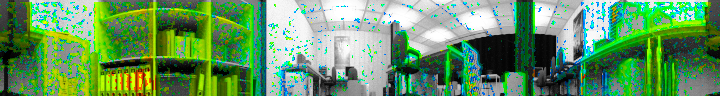
\includegraphics[width=0.825\textwidth]{media/temporal_aliasing_01.png}
  }
  \subbottom[With coarse-to-fine refinement \label{fig:temporal_aliasing_02}]{
    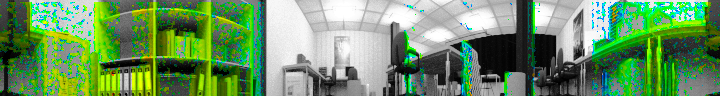
\includegraphics[width=0.825\textwidth]{media/temporal_aliasing_02.png}
  }
  &
  \subbottom[\label{fig:temporal_aliasing:scale}]{
    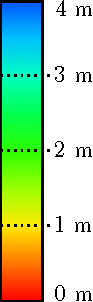
\includegraphics[width=0.08975\textwidth]{media/depth_scale_vert.pdf}
  }
  \end{tabular}
  \caption{Effects of coarse-to-fine refinement. Notice the mismatches originating from temporal aliasing in the lower left image region of (a) (book shelf). In (b) these mismatches are mostly eliminated by applying the coarse-to-fine refinement. Additionally, the pruning introduced with the coarse-to-fine refinement excludes ``uninteresting'' image regions from the depth reconstruction. As seen in the book shelf region in (b) this pruning might sometimes be oversensitive. (c) Shows the color-to-distance mapping used in the images.}
\end{center}
\end{figure}

Temporal aliasing is also a problem in the depth reconstruction algorithm and its implicit optical flow calculation. The ambiguous minima may result in high velocity flow vectors and falsely classified ``near'' objects, which in return cause false-positive obstacle points. See figure \ref{fig:temporal_aliasing_01} for an example of mismatches and the resulting depth in repetitive regions.

The coarse-to-fine approach described above is applied to the depth reconstruction algorithm as follows:
\begin{enumerate}[1.]
 \item Calculate a Gaussian pyramid for both the snapshot and the current view image. Let the number of pyramid levels be $n$.
 \item Pyramid level $\ell = 1$: Perform a complete depth reconstruction on the coarsest pyramid level resulting in the depth field $\img{R}_1(\vec p)$.
 \item Pyramid level $1 < \ell \leq n$: Perform the depth reconstruction on the next finer pyramid level. For every pixel $\vec p$, limit the search range $I_{\vec p}$ in the minimum error search to an interval around the last depth as stored in $\img{R}_{\ell - 1}(\vec p)$. This search range (given as error stack indices) could for example be chosen as
 \begin{equation}
  I_{\vec p, \ell} = \left\{\left\lceil i_\ell(\img{R}_{\ell - 1}(\vec p)) - \kappa\right\rceil, \ldots, \left\lfloor i_\ell(\img{R}_{\ell - 1}(\vec p)) + \kappa - 1\right\rfloor\right\} \cap \left\{0, \ldots, i^{MAX}_\ell\right\}
  \label{eqn:index_range_general} \; .
 \end{equation}
 The parameter $\kappa$ defines the breadth of the search range around the last index. The function $i_\ell(r)$ returns the error stack index for a certain depth value $r$ and a pyramid level index $\ell$. Note that $i_\ell(r)$ varies for all $\ell$, as the image resolution changes (due to subsampling) and so does the count of error stack layers $i^{MAX}_\ell$. This results from the fact that the maximum horizontal shift between two error stack layers is always set to one pixel (section \ref{sec:error_stack}), but the pixel resolution differs between the pyramid levels.
\end{enumerate}
Note that this approach differs from the original coarse-to-fine refinement scheme: The individual pyramid levels are not warped according to the last flow vector field. This warping was performed in order to reduce the maximum landmark velocity and to conform with the Nyquist-Shannon sampling theorem. Yet limiting the search range in the one dimensional minimum error search --- and thus the maximum flow vector length --- has the same effect.

\subsection{Implementation remarks}

\label{sec:coarse_to_fine_implementation}

\begin{figure}[t]
 \begin{center}
  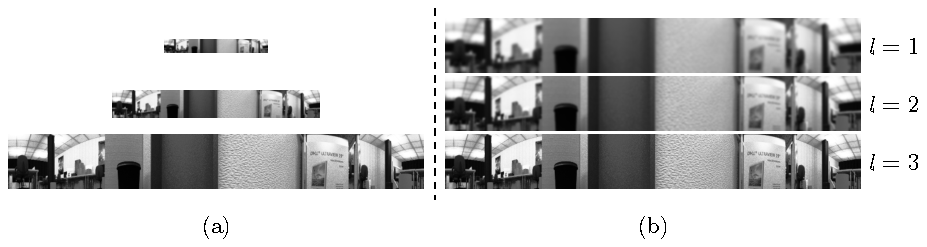
\includegraphics[width=0.975\textwidth]{media/resolution_pyramid.pdf}
 \end{center}
 \caption{Example of the resolution pyramid used in the algorithm. (a) shows the subsampled images for each pyramid level, while (b) contains the low-pass filtered images. Only octaves of the scale space are chosen, resulting in both the low-pass frequency and the image resolution (according to the Nyquist-Shannon sampling theorem) being doubled in each step.}
 \label{fig:resolution_pyramid}
\end{figure}

This section contains a few remarks regarding the actual coarse-to-fine refinement implementation.

\paragraph{Pyramid construction:} The first step in the coarse-to-fine refinement is to construct a Gaussian resolution pyramid for both the snapshot and the current view image. In contrast to the complete scale space pyramid used in SIFT \citep{Lowe04distinctiveimage}, only octaves are selected from the scale space, as depicted in figure \ref{fig:resolution_pyramid}. The scaled images are constructed by low-pass filtering the input images with a $5 \times 5$ binomial convolution kernel and then omitting even rows and columns. As a result, a subsampled image with halved width and height is generated\footnote{This behavior is implemented in the OpenCV \texttt{pyrDown} function.}. This process is repeated until the smallest resolution level is reached. In the current implementation three pyramid levels are generated, reaching from an input resolution of $720 \times 96$ pixels down to $180 \times 24$ pixels.

It is important to note that the first order derivatives of the images used for input dimensionality augmentation (see section \ref{sec:preprocessing}) have to be separately calculated for each resolution level and must not be downsampled along with the input image. This approach allows to reveal large scale gradients in the image and hence improves the matching between $\img{SS}$ and $\img{CV}$.

\paragraph{Simplified index range calculation:} Due to the convention in section \ref{sec:error_stack} to choose a maximum horizontal shift per error stack layer of one pixel, halving the width/height between two resolution pyramid levels also halves the count of error stack layers. An error stack index $i_{\ell - 1}$ in pyramid level $\ell - 1$ corresponds to the same distance $r$ as the error stack index $2  \cdot i_{\ell - 1}$ in pyramid level $\ell$. Consequently the index range equation \ref{eqn:index_range_general} can be reformulated as 
\begin{equation}
 I_{\vec p} = \{2 \cdot \img{J}_{\ell - 1}(\vec p) - \kappa, \ldots, 2 \cdot \img{J}_{\ell - 1}(\vec p) + \kappa - 1\} \cap \{0, \ldots, i^{MAX}_\ell\}
 \label{eqn:index_range} \;.
\end{equation}
Note that the unrefined index field $\img{J}$ is used, as the rounding in equation \ref{eqn:index_range_general} would undo the effects of the refinement. Consequently the index refinement and the index-to-depth steps can be skipped for all resolution layers $\ell < n$.

The concrete implementation additionally guarantees $|I_{\vec p}| = 2\kappa$. This is ensured in a correction step performed after clipping to $\{0, \ldots, i_\ell^{MAX} \}$ (not represented in the equation for sake of simplicity, see figure \ref{fig:index_ranges} instead).

\paragraph{Index range representation:}

Locally limiting the search range of each pixel turns out to be problematic from a runtime point of view. Besides the memory footprint needed for storing the index ranges it would also hinder a SIMD implementation of the minimum error search. By definition, SIMD instructions can only be used if the same operation is performed on blocks of data --- which is certainly not true if each pixel potentially needs to be compared to a different range of reference values. Even in a non-SIMD implementation, the additional branching and memory access could potentially outweigh the benefit of being capable to skip some (relatively cheap) comparisons.

A solution is to store the index range column- instead of pixelwise. The index range $I_\beta$ for column $\beta$ is then calculated as
\begin{align}
 \breve I_{\beta} &= \bigcup_{\gamma} I_{(\beta, \gamma)} \label{eqn:index_range_column_cup} \; , \\
 I_{\beta} &= \{\min(\breve I_{\beta}), \ldots, \max(\breve I_{\beta})\label{eqn:index_range_column}\} \; .
\end{align}
Using this index range for all pixels in a column may lead to problems if the indices are subject to high variance (see figure \ref{fig:index_ranges} for an example). In this case, there is no restriction in the flow vector length and the column is open to the problems caused by temporal aliasing.

\begin{figure}[tb]
 \begin{center}
  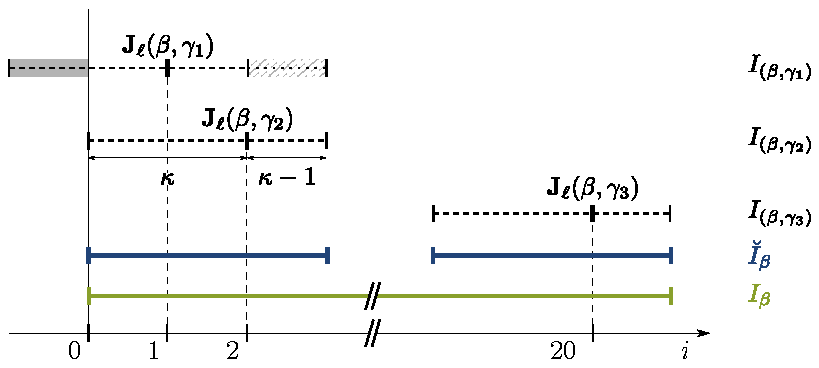
\includegraphics[width=0.975\textwidth]{media/index_ranges.pdf}
 \end{center}
 \caption{The index range calculation as stated in equations \ref{eqn:index_range_column_cup} and \ref{eqn:index_range_column}. The individual pixel index intervals from column $\beta$ are joined, resulting in the auxiliary set $\breve I_\beta$. The minimum and maximum values of $\breve I_\beta$ are then used to build the final column index range $I_\beta$. The gray areas surrounding the interval at pixel $(\beta, \gamma_1)$ visualize the ``breadth constancy'' employed in the implementation (for sake of simplicity not present in the equations). Note how high variances in the indices can cause very large index ranges.}
 \label{fig:index_ranges}
\end{figure}

\paragraph{Runtime improvements and pruning:}

\begin{figure}[h]
  \begin{center}
   \subbottom[Currentview image $\img{CV}$]{
    \begin{tabular}{c}
     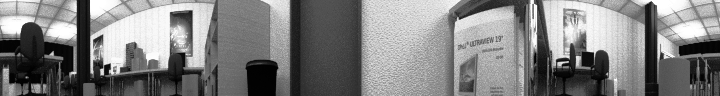
\includegraphics[width=0.9\textwidth]{media/pyramid/cv.png}
    \end{tabular}
   }
   \subbottom[Indices for $\ell = 1$, $180 \times 24$ px, $8$ error stack layers]{
    \begin{tabular}{c}
    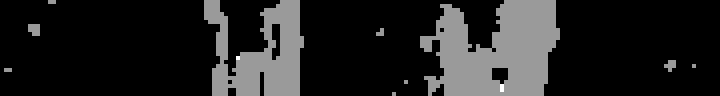
\includegraphics[width=0.9\textwidth]{media/pyramid/indices2_edited.png}\\
    
\includegraphics[width=0.9\textwidth]{media/pyramid/indexRange2.png}
    \end{tabular}
   }
   \subbottom[Indices for $\ell = 2$, $360 \times 48$ px, $16$ error stack layers]{
    \begin{tabular}{c}
    
\includegraphics[width=0.9\textwidth]{media/pyramid/indices1_edited.png}\\
    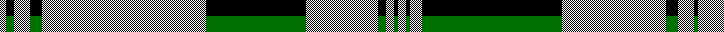
\includegraphics[width=0.9\textwidth]{media/pyramid/indexRange1.png}
    \end{tabular}
   }
   \subbottom[Refined indices for $\ell = 3$, $720 \times 96$ px, $32$ error stack layers]{
    \begin{tabular}{c}
    
\includegraphics[width=0.9\textwidth]{media/pyramid/indices0_edited.png}\\
    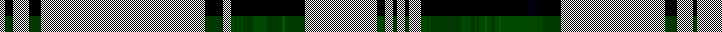
\includegraphics[width=0.9\textwidth]{media/pyramid/indexRange0.png}
    \end{tabular}
   }
  \end{center}
  \caption{Exemplary visualization of the coarse-to-fine refinement. (a) shows the reference current view image. (b)-(d) show the indices resulting from the depth reconstruction algorithm in varying resolutions. In contrast to the last resolution level in (d), the index fields in (b) and (c) have no index refinement applied to them. The small images visualize the index range of each individual column. The first (in this case black) row depicts the start index, the second (green) row the end index encoded as brightness relative to the total count of error stack layers. Note how the relative percentage of used error stack layers decreases with each resolution level. The gray/checkered regions depict pruned columns.}
  \label{fig:coarse_to_fine_pyramid}
\end{figure}

The coarse-to-fine refinement leads to a significant reduction of the runtime as the error stack layers only need to be calculated in the regions actually required for higher resolution levels.

An additional runtime optimization is given by pruning ``uninteresting'' parts of the image from the error stack calculation and the minimum error search (see also figure \ref{fig:coarse_to_fine_pyramid}). ``Uninteresting'' hereby refers to image regions containing no close obstacles. This can be easily accomplished by excluding all image columns $\beta$ from the calculation where $\img{J}_{\ell}(\beta, \gamma) = 0 \; \forall \; \gamma$.

Possibly undesired effects of this pruning can be seen in figure $\ref{fig:temporal_aliasing_02}$, where on the one hand noise is greatly reduced, but on the other hand interesting parts (although with a relatively high distance) are also pruned.

\section{Flow template calculation}

\label{sec:flow_template_calculation}

The most important concept in the optimized implementation of the abstract depth reconstruction algorithm is the computation of so-called ``flow templates''. In essence these contain the precomputed motion field vectors which are needed to warp the snapshot images. 

\subsection{Motion field parameter space reduction}

\begin{figure}[tbp]
\begin{center}
 \subbottom[Plot of $\vec u(\vec p; T(d, \alpha, \psi), r)$ for $d = 0.1 \; \mathrm{m}$, $\alpha = 0.0$, $\psi = 0.0$, $r = 1.0 \; \mathrm{m}$]{
 \includegraphics[width=0.975\textwidth]{{media/flow/flow_lines_d0.10_alpha0.00_psi0.00_r1.00}.pdf}}
 \subbottom[Plot of $\vec u(\vec p; T(d, \alpha, \psi), r)$ for $d = 0.0 \; \mathrm{m}$, $\alpha = 0.0$, $\psi = 0.1$, $r = 1.0 \; \mathrm{m}$]{
 \includegraphics[width=0.975\textwidth]{{media/flow/flow_lines_d0.00_alpha0.00_psi0.10_r1.00}.pdf}}
 \subbottom[Plot of $\vec u(\vec p; T(d, \alpha, \psi), r)$ for $d = 0.1 \; \mathrm{m}$, $\alpha = 0.0$, $\psi = 0.1$, $r = 1.0 \; \mathrm{m}$]{
 \includegraphics[width=0.975\textwidth]{{media/flow/flow_lines_d0.10_alpha0.00_psi0.10_r1.00}.pdf}}
 \subbottom[Plot of $\vec u(\vec p; T(d, \alpha, \psi), r)$ for $d = 0.1 \; \mathrm{m}$, $\alpha = 1.0$, $\psi = 0.0$, $r = 1.0 \; \mathrm{m}$]{
 \includegraphics[width=0.975\textwidth]{{media/flow/flow_lines_d0.10_alpha1.00_psi0.00_r1.00}.pdf}}
\end{center}
\caption{Plots of the motion field $\vec u(\vec p; T(d, \alpha, \psi), r)$ for varying parameters. (a) Shows a pure translatory movement, with focus of expansion (FOE) at $\beta = 0$ and focus of contraction (FOC) at $\beta = \pi$. (b) Shows a pure rotational movement. (c) Shows the combination of both the translatory and the rotational movement. Note how the to motion fields from (a) and (b) are just additively combined. (d) Shows a pure translatory movement with $\alpha \neq 0$. Note how the FOE at $\beta = \alpha$ and FOC at $\beta = \alpha + \pi$ correspond to the movement direction defined by $\alpha$. This is equivalent to a coordinate transformation in $\beta$.}
\label{fig:motion_field_plots}
\end{figure}

Calculating the motion field $\vec u(\vec p; T(d, \alpha, \psi), r)$ for each set of motion parameters $d, \alpha, \psi$, depth step $r_i$ and pixel $\vec p = (\beta, \gamma)$ as stated in the abstract algorithm is not reconcilable with the real-time constraint, as the motion field equation contains numerous trigonometric functions which are relatively slow to evaluate due to their transcendental nature. However, precalculating the motion field vectors in the given form is infeasible as a six-dimensional parameter space $(\beta, \gamma, d, \alpha, \psi, r)$ has to be covered. Consequently the parameter space dimensionality needs to be reduced.

The parameters $d$ and $r$ are not independent. In fact, the flow vector field only depends on the ratio of the two parameters. A graphical motivation can be seen in figure \ref{fig:cylinder_coordinates_transformation}, where the flow vector depends on the triangle formed by $r$ and $d$. Scaling this triangle does not change the flow vector. A proof is given in appendix \ref{proof:flow_subst}. Thus a new parameter $\rho$ can be introduced which expresses the ratio between the two values:
\begin{equation}
 \vec u(\vec p; T(d, \alpha, \psi), r) = \vec u(\vec p; \alpha, \psi, \rho) \text{ where } \rho := \frac{d}{r} \; .
\end{equation}
This substitution was originally presented in the related warping algorithm for visual homing \citep{franz1998did}.

\paragraph{Eliminating the rotational movement:} The motion parameters $\alpha$ and $\psi$ describe the rotational movement that was executed by the robot. It can be shown (see \ref{proof:rot_motion_elim} for a proof), that varying $\alpha$ applies an affine coordinate transformation to the $\beta$-component and $\psi$ is an additive term on the $\beta$ component:
\begin{equation}
 \vec u(\vec p; \alpha, \psi, \rho) = \vec u(\vec p - (\psi + \alpha, 0)^T; \rho) - (\psi, 0)^T
 \label{eqn:rot_motion_elim} \; .
\end{equation}
See figure \ref{fig:motion_field_plots} for an example. This equation can be interpreted as elimination of the rotational movement by panoramic image alignment:
\begin{itemize}
 \item $\psi$ expresses the change in orientation between $\img{SS}$ and $\img{CV}$. Due to the nature of the panoramic images, this change in orientation can be eliminated by a simple horizontal translation of the snapshot image $\img{SS}$.
 \item $\alpha$ denotes the movement direction and by implication the position of the focus of expansion (FOE) in the image. Accordingly, $\alpha$ can be set to zero, if both the snapshot $\img{SS}$ and current view $\img{CV}$ are shifted by $\alpha$ in such a way that the observed FOE and FOC (focus of contraction) positions in $\img{CV}$ match their positions in the non-rotated motion field.
\end{itemize}
Hence using correct image alignment allows to reduce the parameter space by setting $\alpha = \psi = 0$. The resulting motion field equation becomes:
\begin{equation}
  \vec u((\beta, \gamma)^T; \rho)
  = \begmat
    \atantwo
      \left(\sin(\beta), \cos(\beta) + \rho\right) - \beta \\
    \arctan
      \left(
	\frac{
	\tan(\gamma)
      }{
      \sqrt{
    (\cos(\beta) + \rho)^{2} +
    \sin(\beta)^{2}}
      }
    \right) - \gamma
  \finmat
  =
  \begmat
    \beta' - \beta \\
    \gamma' - \gamma
  \finmat
  \label{eqn:flow_template} \; .
\end{equation}
It should be noted that the $\beta$-component of $\vec p_{\img{SS}} = (\beta', \gamma')^T$ does not depend on $\gamma$: For a constant $\rho$, all pixels in a column in $\img{SS}$ are mapped to a single column in $\img{CV}$, yet a non-linear scaling in $\gamma$-direction is applied. This property will allow the linear interpolation needed for calculating the warped $\img{SS'}_i$ to be separated into a horizontal and a vertical interpolation step (see section \ref{sec:motion_field_separability}).

\subsection{Parameter selection, index to depth conversion and distance variance}

\label{sec:index_to_depth}

\paragraph{Flow template definition:} In the last two steps the parameter space was reduced to three parameters $\beta, \gamma$ and $\rho$. This allows precalculating the motion field vectors for each pixel $\vec p = (\beta, \gamma)^T$ and a set of $n$ values of $\rho_i$ where $0 \leq i \leq n - 1$. The snapshot images can then be warped according to these motion vectors, subsequently called \textit{flow templates}. A single flow template at index $i$, $\img{U}_{i}$, is a $h \times w$ matrix containing two-dimensional vectors as its entries:
\begin{equation}
  \img{U}_i(\vec p) = \vec u(\vec p; \rho_i)
  \label{eqn:flow_template_definition} \; .
\end{equation}

\paragraph{Selection of $\rho_i$:} In section \ref{sec:error_stack} it was stated that the $r_i$ should be chosen in such a way that the maximum horizontal shift between two consecutive motion fields is about one pixel. This was motivated by the ability to exploit the complete horizontal resolution that is available in the images.

In the new motion field equation, the motion vector length in pixels solely depends on the parameter $\rho$. Thus the $\rho_i$ have to be selected with the same consideration. As shown in appendix \ref{proof:max_horz_shift} choosing, $\rho_i$ as a multiple of the horizontal angular image resolution (with $w$ being the image width in pixels)
\begin{equation}
  \rho_i = \frac{2 \pi}w \cdot i
\end{equation}
approximately fulfills this requirement for small $i$. Note that for large $i$ this means that the ``one pixel per step'' condition might by violated. In practice $d$ should always be significantly smaller than $r$, as the algorithm is designed for short distances between consecutive snapshot images. Large $d$ would imply near landmarks to be viewed from two completely different directions in the $\img{SS}$, $\img{CV}$ pair.

\paragraph{Index to depth conversion:} The distance function $r(j)$ needed for conversion from continuous index- to world-space is now given as
\begin{equation}
  r(j; d) = \frac{d}{\rho(j)} = \frac{d}j \cdot \frac{w}{2 \pi} \; .
\end{equation}


\paragraph{Calculation of $\sigma_r$:} The choice of $\sigma_r$ was left open in section \ref{sec:prob_landmarks}. Now that the index-to-depth function $r(j)$ has been selected, the corresponding variance $\sigma_r$ can be calculated, which is proportional to the error $\Delta r(j)$. Assuming an index-space error $\Delta j$ and eliminating $j$ yields:
\begin{equation}
  \Delta r(j) = \left| \frac{\partial r(j)}{\partial j} \right| \cdot \Delta j = \frac{d}{j^2} \cdot \Delta j \cdot \frac{w}{2 \pi} = \frac{r(j)^2}{d} \cdot \Delta j \cdot \frac{2 \pi}{w}
\end{equation}
Thus the variance $\sigma_r$ quadratically depends on $r$:
\begin{equation}
\sigma_r \propto \frac{r^2}{d} \label{eqn:sigma_r}
\end{equation}

\chapter{Implementation}

This chapter focuses on the actual implementation of the algorithm and the \textit{implementation-level} optimizations, which --- along with the \textit{algorithm-level} optimizations presented in the previous chapter --- allow for the real-time execution of the algorithm.

First a short introduction to the utilized SSE instruction set extension is given, followed by the techniques employed in the acceleration of the error stack calculation, which include a rearrangement of the snapshot memory along with a separation of the required bilinear interpolation. The next section focuses on the minimum error search and the index space refinement, where a coordinate transformation is applied in order to reduce the required bit depth and to simplify the calculation of the quadratic approximations. The last section describes a fast version of the local environment map for which the Gaussian probability distributions are precalculated for a discrete parameter set.

\section{Short introduction to SSE}

SSE (Streaming SIMD Extensions) is one of the families of SIMD instruction set extensions available on x86- and x64-processors. The original SSE instructions were expanded by incremental updates, namely SSE\,2, SSE\,3, SSSE\,3, SSE\,4.1 and SSE\,4.2. The target platform supports all extensions up to SSSE 3. This implementation will mostly make use of the integer instructions provided by SSE 2 and SSSE 3.

SSE adds sixteen (eight on 32-bit platforms) new 128-bit registers to the processor, which may either hold two double- or four single-precision floats or $4 \times 32$-bit, $8 \times 16$-bit or $16 \times 8$-bit integers, thus allowing up to $16 \times$ parallel execution on a single processor core. The data layout solely depends on the instructions used on these registers. A 128-bit data block is hereinafter referred to as \textit{SSE word}.

The SSE instructions can be accessed in high level programming languages using so called \textit{intrinsics}, which behave like normal functions operating on a 128-bit data type (\texttt{\_\_mm128i} for integers, \texttt{\_\_mm128d} for doubles and \texttt{\_\_mm128} for singles) but receive special handling from the compiler and are (most of the time) translated into a single SSE instruction.

See the \textit{Intel 64 and IA-32 Architectures Optimization Reference Manual} \citep{IntelOptimizationHandbook} for more information on this topic.

\section{Error stack calculation}

\label{sec:error_stack_sse}

This section focuses on the optimizations that allow a very fast calculation of the error stack layers $\img{E}_i$. These optimizations include a special snapshot memory layout suitable for SSE as well as exploiting the separability of the motion field equation.

\subsection{Snapshot memory layout}

\begin{figure}[tb]
 \begin{center}
  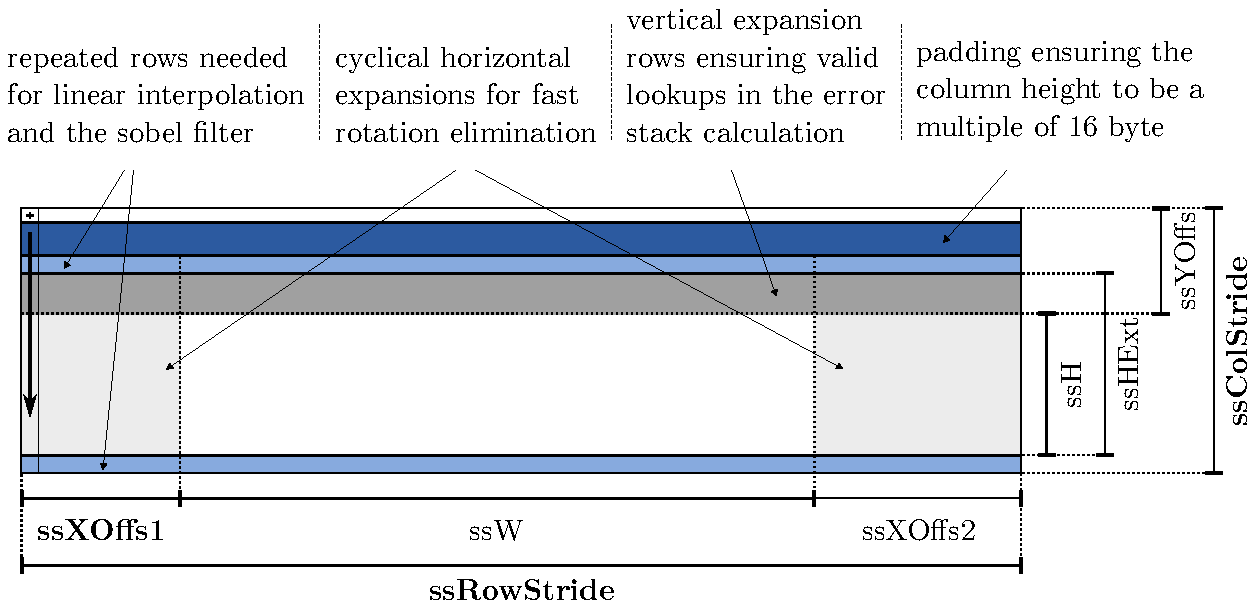
\includegraphics[width=0.975\textwidth]{media/memlayout_snapshot2.pdf}
 \end{center}
 \caption{Snapshot memory layout. Each resolution level and each snapshot component is stored according to the scheme shown above. The cross in the top left corner marks the origin, the arrow indicates the column-major memory layout. Bold labels represent values which are chosen as multiples of sixteen. The actual data used for the error stack calculation is stored in the white area in the middle of the image.}
 \label{fig:memlayout_snapshot2}
\end{figure}

\label{sec:memory_layout}

Incoming panoramic snapshot images are rearranged in memory according to a special memory layout scheme which meets the demands of the SSE implementation. This rearrangement is employed after the resolution pyramid has been calculated (see section \ref{sec:coarse_to_fine_implementation}). Once the first stage of the rearrangement has been performed (except for the transpose and horizontal expansion step, see below) the first derivatives in $x$- and $y$-direction are approximated using a $3\times3$-Sobel filter. The resulting image components (intensity, $x$-derivative, $y$-derivative) are stored individually as independent images. This corresponds to the so called \textit{structure of arrays} (SoA) paradigm, which in conjunction with SSE performs better for most applications than the classical \textit{array of structures} (AoS) \citep[chapter 4.5.1, ``data structure layout'']{IntelOptimizationHandbook}.

\paragraph{Column-major layout:} The first design decision regarding rearrangement includes a conversion from the standard row-major to a column-major memory format (hence the image is stored transposed). A column-wise processing enables the efficient interpolation scheme presented below (see section \ref{sec:motion_field_separability}). In order to save memory (and thus expensive memory access), the bit depth of the input images remains unchanged and each pixel is stored as an 8-bit unsigned integer.

By adding padding-rows, it is ensured that the column height is a multiple of 16 bytes. This is important, as SSE load instructions work most efficiently if the memory addresses are aligned to 16-byte boundaries \citep[chapter 4.4, ``stack and data alignment'']{IntelOptimizationHandbook}. Additionally, this allows each column to be handled with an integral count of SSE words.

\paragraph{Horizontal rotation elimination borders:} In order to facilitate the rotational motion elimination described in equation \ref{eqn:rot_motion_elim}, the snapshot image is cyclically extended in $x$-direction. As the panoramic images are cyclic in horizontal direction this allows the rotational motion elimination to be reduced to two horizontal offsets for the current view and the snapshot images.

However, the maximum rotational angle that can be eliminated is now limited by the width of the cyclic extension, which is currently chosen as $\frac{w}4$ in both directions, limiting the maximum rotation angle to $\pm 90^\circ$ (which should be sufficient). It should also be noted that the use of discrete pixel offsets introduces a quantization error with respect to the rotation angle, which is especially large for lower resolution levels.

\paragraph{Vertical lookup extension:} As noted in section \ref{sec:panoramic_image}, only a portion of the polar range available in the snapshot is effectively used for the actual depth reconstruction. The preprocessing step only copies this reduced portion, yet as warping the snapshot requires lookups which lie outside this reduced polar range (see figure \ref{fig:flow_template_regions}), some additional vertical extension rows allowing these lookups are added to the top of the snapshot. The height of this extension region is chosen to be as large as possible (only rows that are present in the input image are copied) and as small as needed (only rows that are referenced by the longest flow vector are copied).

If the polar range covered by the input image is too small, the vertical lookup region does not eliminate the need of adding some mechanism to the error stack calculation that allows to cope with such invalid lookups.

A copy of the top row is added to the top of the snapshot data and the same procedure is analogously performed at the bottom. This allows to prevent branching in the border regions for the linear interpolation and the Sobel–kernel application.

\paragraph{Memory layout descriptors:}

A schematic showing the complete memory layout can be seen in figure \ref{fig:memlayout_snapshot2}. The annotated widths and heights fully describe the memory layout and together form a \textit{memory layout descriptor}. These descriptors (also including the flow template and error stack memory layout data not described here) are calculated once for each pyramid level. A pointer to the memory descriptor is then passed to all parts of the implementation.

\subsection{Separability of the motion field equation}

\begin{figure}[tb]
 \begin{center}
  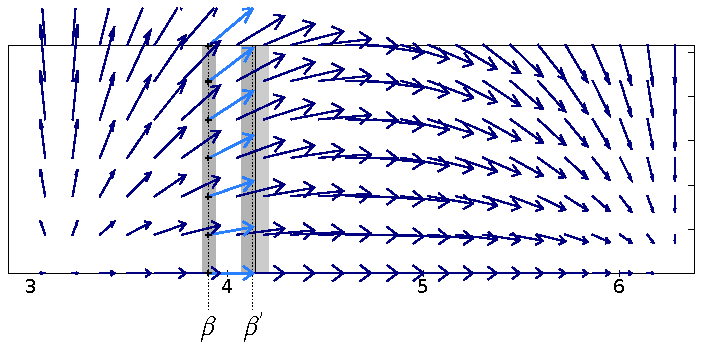
\includegraphics[width=0.75\textwidth]{media/flow_template_lookup.pdf}
 \end{center}
 \caption{Section of a flow template $\img{U}_i$. The highlighted arrows point from a target column $\beta$ (corresponding to a discrete pixel) to the source column $\beta'$. As all arrows point to the same source row, the bilinear interpolation employed when calculating the warped image $\img{SS'}_i$ can be split into a \textit{horizontal} interpolation step (interpolating between the two referenced source rows) and a \textit{vertical} interpolation step.}
 \label{fig:flow_template_lookup}
\end{figure}

\label{sec:motion_field_separability}

The motion field equation \ref{eqn:flow_template} as given in section  \ref{sec:flow_template_calculation} describes the mapping of a target pixel $(\beta, \gamma)$ in $\img{SS'}_i$ (needed for the error stack calculation, see section \ref{sec:error_stack}) to a source pixel $(\beta', \gamma')$ in $\img{SS}$. Thus the $\img{SS'}_i$ are calculated by warping the snapshot image $\img{SS}$ according to the flow template $\img{U}_i$ using bilinear interpolation. As noted above, the source column $\beta'$ solely depends on the target column $\beta$ and not on the target row $\gamma$.

Column-wise calculation of each discrete target column $\beta$ allows for separation of the bilinear interpolation into a \textit{horizontal} and a \textit{vertical} interpolation step. For the horizontal interpolation, the two neighboring source columns referenced by $\beta'$ are interpolated, resulting in an intermediate source column. In the vertical interpolation step for each row $\gamma$ in $\beta$ the two source pixels referenced by $\gamma'$ in the intermediate source column are interpolated (see figure \ref{fig:flow_template_lookup}).

\subsection{Flow template calculation}

The actual flow template data for all $\img{U}_i$ and all resolution levels are precomputed for each pixel as defined in equation \ref{eqn:flow_template_definition}. In order to simplify the code the depression angle $\check \gamma$ is set to a fixed value of $0^\circ$, while the elevation angle $\hat \gamma$ remains a free parameter.

Instead of storing a field of two-dimensional floating point vectors for each target pixel, the flow template is encoded in memory using a set of five integer arrays:
\begin{itemize}
 \item A one-dimensional 16-bit array \texttt{tarX} (size $w$) holds the index of the left-most of the two discrete source columns corresponding to each target column $\beta$.
 \item A one-dimensional array \texttt{facX} (size $w$) holds the horizontal interpolation factors for the two source columns. The factors are multiplied by $2^6$ and stored as $2 \times 8$-bit tuples. The full 8-bit range is not used in order to prevent overflows in subsequent steps.
 \item A two-dimensional 8-bit array \texttt{offsY} (size $w \times \frac{h}8$) holds the index of the first source pixel (clamped to zero) in the intermediate column for each block of eight pixels in each target column.
 \item For each pixel the two-dimensional 8-bit array \texttt{shuffleMaskY} (size $w \times 2 \cdot h$) holds the two vertical source pixel indices relative to the first source pixel offset stored in \texttt{offsY}. Inaccessible pixels --- those with an index smaller than zero or larger than fifteen --- are marked with 0xFF.
 \item A two-dimensional array \texttt{facY} (size $w \times h$) holds the vertical interpolation factors for the two source pixels corresponding to each target pixel. The values are encoded as described for \texttt{facX}.
\end{itemize}
The two-dimensional arrays are stored column-major and with corresponding padding ensuring the column size to be a multiple of 16. The offsets stored in \texttt{tarX} and \texttt{offsY} directly address the pixels as they are stored in the snapshot memory layout.

\subsection{Snapshot warping and error stack calculation}

\begin{figure}
 \begin{center}
  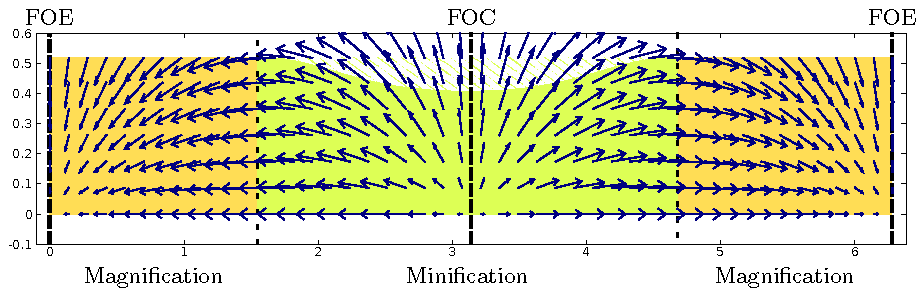
\includegraphics[width=0.975\textwidth]{media/flow_template_regions.pdf}
 \end{center}
 \caption{Regions in each flow template. The $\pi$-interval surrounding the focus of contraction (FOC) describes a \textit{minification} in which the source pixel region is always larger or equal in size to any region of target pixels (many pixels are mapped to few pixels). The $\pi$-interval surrounding the focus of expansion (FOE), however, describes a \textit{magnification} in which the source pixel region is always smaller or equal in size to any region of target pixels (few pixels are mapped to many pixels). The hatched region in the image contains the flow vectors pointing to invalid (out of range) source pixels.}
 \label{fig:flow_template_regions}
\end{figure}

The calculation of a single error stack layer $\img{E}_i$ consists of the following steps: For each snapshot component, a warped version of that component is calculated according to the flow template using bilinear interpolation. Then the absolute difference between the warped image component and the corresponding current view image component is calculated. This value is subsequently added to the resulting error stack layer value (remember that the optical flow as defined in equation \ref{eqn:optical_flow} uses the $L^1$-norm).

\paragraph{Image warping and interpolation:} Given the precalculated flow template, the horizontal and vertical warping and interpolation steps become equally trivial, although the vertical interpolation requires additional attention.

Of special interest in both steps is the SSSE 3 \texttt{\_mm\_maddubs\_epi16} intrinsic, which takes two $16 \times 8$-bit SSE words ($a$ and $b$) as input and calculates a $8 \times 16$-bit output vector $c$ according to the following expression ($[i]$ corresponds to the $i$th cell in the SSE word):
  $$c[i] = a[2 \cdot i] \cdot b[2 \cdot i] + a[2 \cdot i + 1] \cdot b[2 \cdot i + 1] \quad \forall \; 0 \leq i < 8 \; .$$
Interpolation between pixel pairs can be achieved by placing each pair in adjacent cells in $a$ and the corresponding interpolation factors in $b$, allowing eight result pixels to be computed in a single instruction.

The interpolation in horizontal direction is performed by interlacing two $16 \times 8$-bit SSE words read from the source rows into two pixel pair vectors $aLO$ and $aHI$ and interpolating those according to the factors stored in the flow template \texttt{facX} array. The two result vectors are then packed into the 8-bit intermediate column (see appendix \ref{code:horz_interpolation} for the complete code).

Interpolation in vertical direction is done by reading a $16 \times 8$-bit SSE word from the intermediate row starting with the pixel specified in \texttt{offsY} and building a single pixel pair vector by shuffling this 16-pixel input word according to the indices specified in \texttt{shuffleMaskY}. The pixel pairs are then interpolated according to the interpolation factors in \texttt{facY}. Note that this technique is only capable of mapping a maximum of 16 consecutive source pixels to 8 target pixels, so the minification factor should never exceed two (see figure \ref{fig:flow_template_regions}). Yet for the parameters used in practice this is never the case.

For invalid pixel lookups --- those marked with 0xFF in the shuffle mask --- a ``maximum error mask'' is created from the shuffle mask and the corresponding error values are set to this maximum error value. As three image components are processed and the maximum pixel intensity difference is 255 per component, this maximum error value is chosen as 0x3FF (see \ref{code:vert_interpolation} for the complete code).

\paragraph{Error stack bias:} The error bias $\tau \cdot i$ introduced for the minimum error search in section \ref{sec:minimum_error_search} is directly added to the error values in each error stack layer $\img{E}_i$ and will thus not be regarded in the following sections.

\section{Index field calculation}

The next step in the algorithm is to find the minimum error in the error stack layers and to generate the index field $\img{J}$, which is then refined to the index field $\img{\tilde J}$. Yet before these steps can be discussed in detail, an error propagation matrix $W_{\vec p}$ (left open in section \ref{sec:minimum_error_search}) needs to be chosen.

\subsection{Propagation matrix and minimum error search}

\label{sec:propagation_matrix_choice}

The most influential parameter from an efficiency point of view is the propagation matrix $W_{\vec p}$. The space and data variant $n \times n$ error propagation matrix (where $n = 2 \cdot r_W + 1$) introduced in section \ref{sec:convolution_kernels} is generally non-separable and thus needs $n^2$ calculations in every pixel. Additionally, creating and storing the filter kernels requires additional time and storage.

Preceding experiments (see section \ref{sec:results_propagation} for the results and chapter \ref{sec:experiments} for the test set-up) have shown that choosing $W_{\vec p}$ as a space-invariant $3 \times 3$ binomial convolution kernel provides an acceptable trade-off between speed and quality. The propagation matrix $W$ is subsequently defined as:
  $$W := W_{\vec p} = \frac{1}{16} \cdot \begmat 1 & 2 & 1 \\ 2 & 4 & 2 \\ 1 & 2 & 1 \finmat \; .$$
The filter is separable into a horizontal and vertical convolution
  $$W := \frac{1}{16} \cdot \begmat 1 & 2 & 1 \finmat \ast \begmat 1 \\ 2 \\ 1 \finmat$$
which can both be trivially implemented using SSE.

\paragraph{Minimum error search:} The minimum error search leading to the index field $\img{J}(\vec p)$ is implemented exactly as defined in equation \ref{eqn:kernel_minimum_search_bias}: First $\img{E}_i \ast W$ is calculated for all error stack layers (which as noted above already contain the bias $\tau \cdot i$), then for each pixel $\vec p$ the layer index with minimum error is searched. Using SSE, eight pixels can be processed at a time. In order to allow for a refinement of the index field, the indices are stored as 16-bit fixed point numbers with the scale factor $2^8$.

\subsection{Index field refinement}

In equation \ref{eqn:index_field_refinement} the refined index field $\img{\tilde J}$ was effectively defined as
\begin{equation}
\img{\tilde J}(\vec p) = \argmin_{\img{J}(\vec p) - 1 \leq j \leq \img{J}(\vec p) + 1}
  \left( \check E_{\vec p}(j) + \check R_{\vec p}(j) \right) \; ,
  \label{eqn:index_field_refinement_impl}
\end{equation}
where $\check E(J)$ refers to the convoluted quadratic error stack approximation functions and $\check R(j)$ to the convoluted regularization functions:
\begin{align*}
   \check E_{\vec p}(j) &= \sum_{\vec q \in A(\vec p)} \omega_{\vec p}^{\vec q} \cdot \tilde E_{\img{J}(\vec p)}(j; \vec q) \; ,
 & \check R_{\vec p}(j) &= \lambda \cdot \sum_{\vec q \in A(\vec p)} \omega_{\vec p}^{\vec q} \cdot (\img{J}(\vec q) - j)^2 \; .
\end{align*}


\paragraph{Simplification of the index field refinement equation:} The convolution over a set of quadratic polynomials is impractical for a fast implementation. It would be of advantage if the convoluted error stack layers $\img{E}_i \ast W$ calculated in the previous step could be reused.

In the case of $\check E_{\vec p}(j)$, the convolution and the calculation of the quadratic coefficients are commutative: For $i \in \{-1, 0, 1\}$ and $j = \img{J}(\vec p)$ the following relation holds
\begin{equation*}
  \check E_{\vec p}(j + i)
  {\overset{\text{Def. }\tilde E\vphantom{\omega_{\vec p}^{\vec q}}}=} \sum_{\vec q \in A(\vec p)} \omega_{\vec p}^{\vec q} \cdot \img{E}_{\img{J}(\vec p) + i}(\vec q) \\
  \overset{\text{Def. }\omega_{\vec p}^{\vec q}}= \left(\img{E}_{\img{J}(\vec p) + i} \ast W\right)_{\vec p}
\end{equation*}
and --- as each quadratic polynomial is uniquely defined by three points --- proves that fitting the coefficients according to the values in the convoluted error stack layers is equivalent to convolving the polynomials themselves.

Unfortunately the regularization function $\check R_{\vec p}(j)$ is not commutative regarding the convolution of the index field $\img{J}$. Expanding $\check R_{\vec p}(j)$ yields
\begin{align*}
  \check R_{\vec p}(j) &= \lambda \cdot \left(
    j^2 - 2 \cdot (\img{J} \ast W)_{\vec p} \cdot j +
    \smash{\sum_{\vec q \in A(\vec p)}} \omega_{\vec p}^{\vec q} \cdot \img{J(\vec q)}^2 \right)\vphantom{\sum_{\vec q \in A(\vec p)}}
\end{align*}
where the constant term plays no role for finding the minimal $j$. Thus an equivalent and commutative regularization function is given by
\begin{equation}
  \tilde R'(j; \vec p) = \lambda \cdot ( j^2 - 2 \cdot \left(\img{J} \ast W \right)_{\vec p} \cdot j)
\end{equation}

\paragraph{Quadratic approximation calculation:}

\begin{figure}[t]
  \begin{center}
   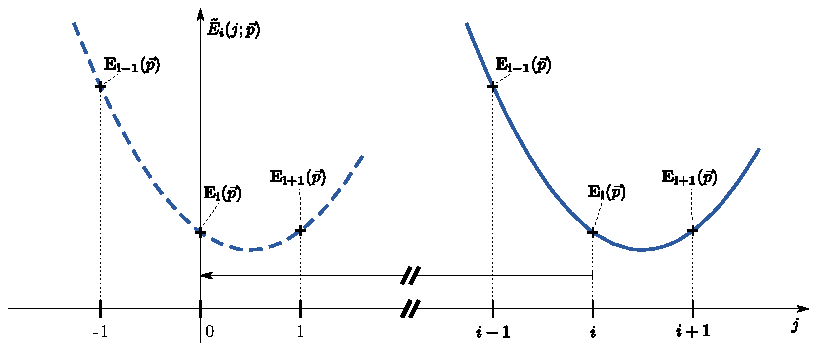
\includegraphics[width=0.975\textwidth]{media/polynomial_coord_trafo.pdf}
  \end{center}
  \caption{Translating the center index $i$ of each quadratic approximation polynomial $\tilde E_i(j; \vec p)$ (solid blue line) to the origin at $0$ (dashed blue line) allows for simplified  calculation of the polynomial coefficients $\vec w$ and lowers the required bit depth needed to store those.}
  \label{fig:polynomial_coord_trafo}
\end{figure}


The calculation of the quadratic polynomials $\tilde E_i(j; \vec p) = (j^2, j, 1) \cdot \vec w$ as given in equation \ref{eqn:polynomial_coeffs} can be simplified by a coordinate transformation which translates the center index $i$ to the origin at $j = 0$ (see figure \ref{fig:polynomial_coord_trafo}). The adapted refinement equation \ref{eqn:index_field_refinement_impl} is then given as
\begin{equation}
\img{\tilde J}(\vec p) =\argmin_{- 1 \leq j \leq 1} \left(
  \check E_{\vec p}(j) + \check R_{\vec p}(j)\right) + \img{J}(\vec p) \; .
\end{equation}
The coefficients $\vec w$ of $\check E_{\vec p}(j)$ can now be trivially implemented in SSE:
\begin{equation}
	\vec w = \begmat w_2 \\ w_1 \\ w_0 \finmat = \frac{1}2
	\begmat
		1 & -2 & 1 \\
		-1 & 0 & 1 \\
		0 & 2 & 0
	\finmat
	\cdot
	\begmat
		\mathbf{E}_{i - 1}(\vec p) \ast W \\
		\mathbf{E}_{i}(\vec p) \ast W \\
		\mathbf{E}_{i + 1}(\vec p) \ast W
	\finmat
	\label{eqn:polynomial_coeffs_impl} \; .
\end{equation}
Additionally, this equation has the advantage of yielding a much smaller coefficient vector, which can (using the SoA paradigm) be stored in three $8 \times 16$-bit SSE words \texttt{w0}, \texttt{w1}, \texttt{w2}, allowing the refinement of eight pixels at the same time.

For the regularization term $\tilde R'(j; \vec p)$ the coordinate transformation yields the following equation
$$\tilde R'(j; \vec p) = \lambda \cdot (j^2 - 2 \cdot (\left(\img{J} \ast W\right)_{\vec p} - \img{J}(\vec p)) \cdot j) \; .$$
Note that for the search range $-1 \leq j \leq 1$ the quadratic term $j^2$ is negligible and the factor two can be condensed into $\lambda$. Thus the regularization is reduced to subtracting $\lambda \cdot (\left(\img{J} \ast W\right)_{\vec p} - \img{J}(\vec p))$ from the linear coefficient vector \texttt{w1}.

All coefficients are stored as fixed point numbers (scale factor $2^3$) allowing a slightly higher resolution for $\lambda$.

\paragraph{Refined index calculation:} The extremum of a quadratic polynomial $w_2 j^2 + w_1 j + w_0$ is given by $\check \jmath = - \frac{w_1}{2 w_2}$. In order to eliminate the need for special handling (which is hardly possible when using SIMD instructions) in the case of $w_2 = 0$, $w_2$ is always set to one in that case. The resulting $\check \jmath$ is clamped to the interval $[-1, 1]$ and the corresponding error value is then compared to the error values at $j = -1$ and $j = 1$. The actual refined index field entry is then chosen as the index belonging to the smallest of the three error values.

As SSE does not provide integer division instructions, the term $-\frac{w_1}{2 w_2}$ is evaluated using floating point numbers. The approximative but significantly faster reciprocal instruction $\texttt{\_mm\_rcp\_ps}$ in conjunction with a multiplication is used here, which has a combined precision in the range of $\approx 2^{-11}$ \citep[chapter 11.12 ``divide and square root operations'', p. 417ff.]{IntelOptimizationHandbook}. This is not a problem since the resolution of the fixed-point 16-bit indices $j$ was chosen as $2^{-8}$.


\section{Local environment map}

The local environment map is especially optimized in the position update and the distribution accumulation as introduced in section \ref{sec:obstacle_detection}. These optimizations are roughly sketched in the two following sections.

\subsection{General optimizations}

The local environment map is stored in memory as a 16-bit two-dimensional matrix. SSE trivially allows to speed up the map decay step (equation \ref{eqn:map_decay}), as the SSSE 3 intrinsic \texttt{\_mm\_mulhrs\_epi16} allows $8\times$ parallel multiplication of a $8 \times 16$-bit word with a scalar $\delta \in (0, 1]$.

Furthermore the need of the image rotation in the map update step was eliminated by integrating the change in orientation $\psi$ and using this current orientation and the current translatory motion direction $\alpha$ as an angular offset when inserting the Gaussian distributions. This allows to reduce the map update step to a discrete, pixel wise translation. The error introduced by rounding to discrete pixel offsets is accounted for by feeding the rounding error into the next map update step (comparable to error-diffusion dithering).

Although the calculation of the thresholded map image can be parallelized using SSE, no trivial optimization of the connected component calculation was found.

\subsection{Distribution accumulation optimization}

\begin{figure}[tb]
 \begin{center}
  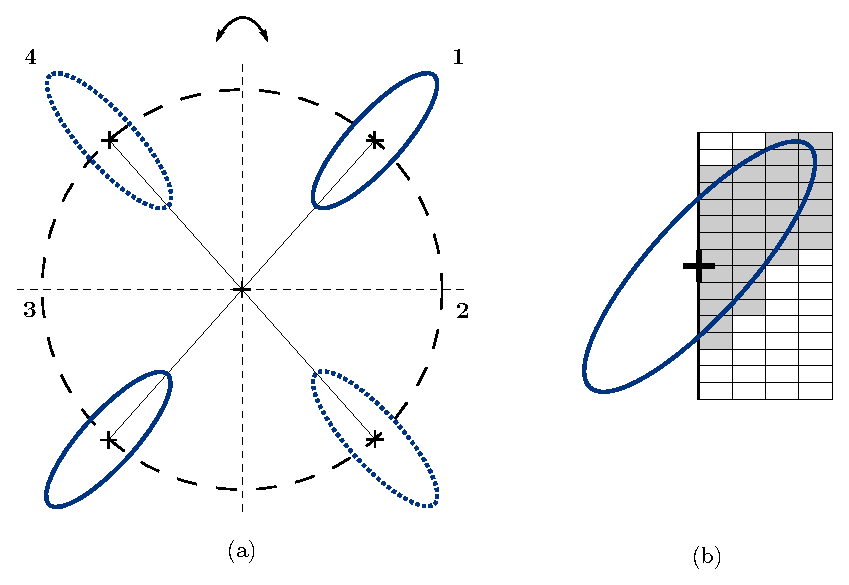
\includegraphics[width=0.975\textwidth]{media/gaussian_distribution_symmetries.pdf}
 \end{center}
 \caption{Symmetries of a Gaussian distribution. (a) A Gaussian distribution calculated for quadrant 1 can be used in quadrant 3 without modification. Mirroring along the $x$-axis allows to use the distribution in quadrant 2 and 4. Consequently precalculating the distributions for one quadrant only allows to reduce the space requirement by one quarter. (b) As each Gaussian distribution is point-symmetric, only one half of the distribution needs to be stored in memory --- the memory footprint can be reduced even more by skipping all SSE words which only contain pixel values below a certain threshold (white).}
 \label{fig:gaussian_distribution_symmetries}
\end{figure}

In order to avoid the costly evaluation of the Gaussian probability distributions whenever a landmark point $\vec q = (\beta, r)$ is inserted into the map, the distributions are precalculated in Cartesian space for discrete $\beta_i \in [0, 2\pi]$ and a discrete range of $r_i \in [r_{\mathrm{MIN}}, r_{\mathrm{MAX}}]$. Note that the variance $\sigma_r$ as derived in equation \ref{eqn:sigma_r} also depends on the translatory distance $d$ between $\img{SS}$ and $\img{CV}$, yet precalculating the distributions for a three-dimensional parameter space $\beta, r, d$ is impractical. Therefore the robot is implicitly assumed to move with constant speed.

As depicted in figure \ref{fig:gaussian_distribution_symmetries}, the distributions are stored as fixed point $8 \times 16$-bit SSE words for a rectangular hull encompassing a contour line at a certain threshold level. To lower the memory requirements symmetries in the distributions are exploited and only SSE words containing values above the threshold level are stored in memory, along with a descriptor that contains the number of words skipped and the number of words in a row. Preceding experiments have shown that the reduced memory footprint and better cache locality outweighs the overhead introduced by this packing scheme.

The map array size is extended by the half width/height of the largest Gaussian distribution bounding rectangle in order to eliminate the need of border handling (and thus branching) when plotting the map pixels.

The SSE code used for accumulating a precalculated distributions onto the local environment map is given in appendix \ref{code:gauss}.


\chapter{Experiments and results}

\label{sec:experiments}

This chapter describes the experiments which have been conducted in order to measure the performance of the obstacle detection algorithm. These experiments include tests in a computer-generated environment as well as real-world tests on the robot platform. For the computer-generated environment quantitative measures describing the performance of the algorithm have been developed.

\section{Environments}

In this section the environments used for testing the algorithm are described. Those environments cover two computer-generated scenes and a real-world test in a living room inspired test room.

\subsection{Computer-generated environments}

\begin{figure}[p]
 \begin{center}
  \subbottom[Apartment scene ($7 \times 5 \; \mathrm{m}$)]{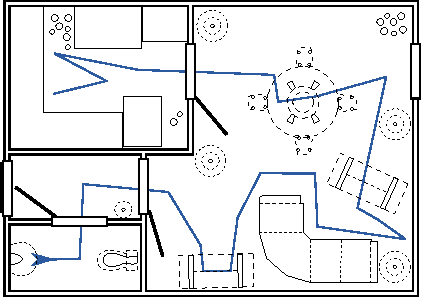
\includegraphics[width=0.6\textwidth]{media/flat_outlines.pdf}}
  \subbottom[Laboratory scene ($10 \times 10 \; \mathrm{m}$)]{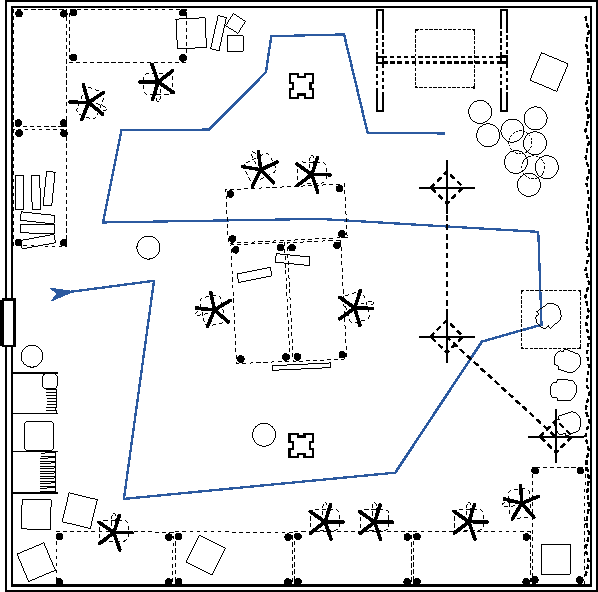
\includegraphics[width=0.85\textwidth]{media/laboratory_outlines.pdf}}
 \end{center}
 \caption{Overview of the computer-generated scenes. Solid lines indicate obstacles relevant to the robot (as they are placed directly on the floor), dashed lines are only for orientation and indicate objects which are too high to be detected as obstacles. The blue line depicts the robot trajectory.}
 \label{fig:floorplan}
\end{figure}

\begin{figure}[t]
 \begin{center}
  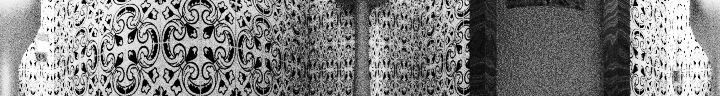
\includegraphics[width=0.49\textwidth]{media/sample_snapshots/flat4.png}
  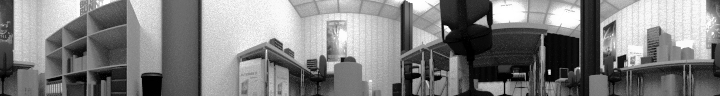
\includegraphics[width=0.49\textwidth]{media/sample_snapshots/lab1.png}
  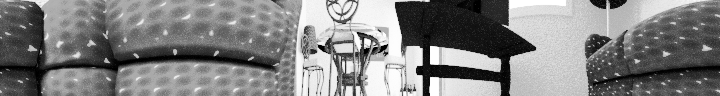
\includegraphics[width=0.49\textwidth]{media/sample_snapshots/flat1.png}
  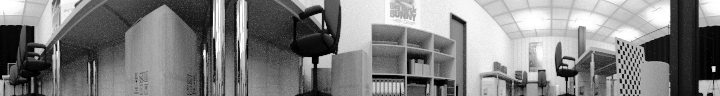
\includegraphics[width=0.49\textwidth]{media/sample_snapshots/lab2.png}
  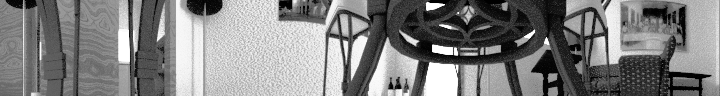
\includegraphics[width=0.49\textwidth]{media/sample_snapshots/flat2.png}
  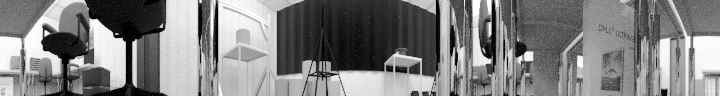
\includegraphics[width=0.49\textwidth]{media/sample_snapshots/lab3.png}
  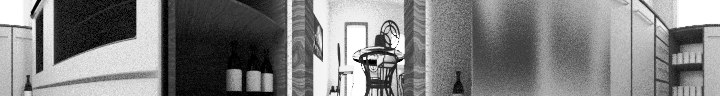
\includegraphics[width=0.49\textwidth]{media/sample_snapshots/flat3.png}
  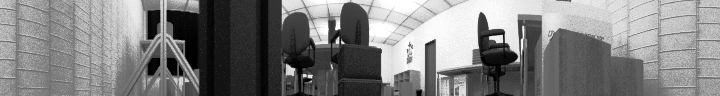
\includegraphics[width=0.49\textwidth]{media/sample_snapshots/lab4.png}
 \end{center}
 \caption{Some exemplary snapshots from the apartment scene (left) and the laboratory scene (right) with applied histogram equalization. The pictures are used as input for the test runs exactly as shown here.}
 \label{fig:sample_snapshots}
\end{figure}

Measuring a perfect ground truth for the depth reconstruction stage of the algorithm in the real-world would be a very tedious task. In computer-generated environments, the ground truth can be simply extracted by storing the so-called $z$-buffer, which contains the distance of each pixel in the scene and is created during the rendering process. Moreover, the computer-generated scenes allow to test the algorithm under a perfect path integration assumption (section \ref{sec:assumptions}) as the position and orientation of the robot are known at all times.

The algorithm is given a sequence of prerendered panoramic snapshot images. These snapshots are generated from the perspective of a virtual robot which moves with constant velocity along a predefined trajectory. The trajectories were laid out by hand, no navigation or obstacle evasion was simulated.

The scenes were modeled and rendered using the open-source software \textit{Blender} and its path-tracing renderer \textit{Cycles}\footnote{See \url{http://www.blender.org/} for more information.}, which was slightly modified in order to produce the required spherical panoramic images. The scenes were rendered under full global illumination. The snapshot resolution is set to $720 \times 96$ pixels and the depression and elevation angles are set to $\check \gamma = 0^\circ$ and $\hat \gamma = 30^\circ$, respectively. The robot travels along the trajectory at $0.2 \, \frac{\mathrm{m}}{\mathrm{s}}$. A new frame is created every $200 \, \mathrm{ms}$. The virtual camera moves at an elevation of $0.1 \; \mathrm{m}$ above the floor. Note that the images contain sampling noise produced by the path-tracer.

Two environments (see figure \ref{fig:sample_snapshots} for example images) were created: A large-scale single-room laboratory scene and a relatively small apartment scene, consisting of bathroom, hallway, living room and a kitchen. See figure \ref{fig:floorplan} for the scene layouts. 

The laboratory scene primarily features two types of table legs (cylindrical brushed metal legs and rectangular dull-white powder-coated legs), chairs, printed cardboard boxes, tripod legs and featureless cylinders as obstacles. Two of the walls (left and right) feature a very fine wallpaper-like structure, the other two walls feature a brick texture. The scene is lit by a total of nine ceiling lights. In order to simulate a realistic computer scientist working environment, the window openings are barred with a light-tight black curtain. The average distance between the robot and the obstacles is relatively high (typically around $\approx 0.5 - 1 \, \mathrm{m}$). The prerecorded trajectory consists of $873$ snapshot images.

The apartment scene features floor lamps, a couch, tables, chairs, bathroom and kitchen interior as well as empty glass bottles in the corners of the room\footnote{The author likes to stress that the apartment scene in no way reflects his own living environment.}. The bathroom is tiled with patterned tiles, while the other walls in the apartment are covered with relatively rough interior wall plaster. The scene is lit through various window openings. The average distance between the camera and the obstacles is relatively small (typically around $\approx 0.2-0.6\,\mathrm{m}$). The prerecorded trajectory consists of $624$ snapshot images.

While the resulting snapshots are not completely photo-realistic, they are believed to be a reasonable approximation.

\subsection{Real-world tests}

Real-world tests are performed on the actual mobile robot platform which runs the fully optimized version of the obstacle detection algorithm. The robot performs a cleaning run in which it seeks to drive parallel lanes in order to cover the complete room. The detected obstacle points are directly fed into the navigation algorithm and influence the robot trajectory. The robot captures a snapshot image approximately every $200 \, \mathrm{ms}$ and moves at a translatory velocity of about $0.2 \, \frac{\mathrm{m}}{\mathrm{s}}$.

The obstacle detection is activated whenever the robot drives straight lanes. It fully relies on odometry data as input for the local motion parameters. In the current implementation, the motion parameters are not integrated between the snapshots. The wheel encoder values are read after an image has been captured and are assumed to be piecewise linear. The odometry data and the snapshot images are recorded for later analysis.

The test room features a living room suite (four chairs, one table, carpet on the floor), a couch, floor lamp, curtain and a sideboard. The room is lit by a single fluorescent ceiling lamp. The floor of the room is covered with wooden planks leading to a slightly uneven floor.

\section{Quality measures}

The simulated test runs are analyzed using quantitative quality measures. These include the count of \textit{true} and \textit{false positive} obstacle points as well as the average obstacle point detection error and the average depth reconstruction error.

\subsection{True and false positive obstacle points}
Let $\img{M_R}$ denote the local environment map as generated by the algorithm containing the reconstructed obstacle points and let $\img{M_T}$ be a reference local environment map, which --- instead of using the reconstructed depth map --- is generated from the ground truth depth map. Note that the depth variance $\sigma_r$ used in the generation of $\img{M_T}$ has to be chosen as a constant value describing the quantization error of the reference depth map (the depth is sampled at 8 bit with a resolution of $0.078 \, \nicefrac{\mathrm{m}}{\mathrm{dig}}$). Additionally, the following sets need to be defined:
\begin{align*}
  P_R &:= \{ \vec p = (x, y)^T \mid \vec p \text{ is reconstructed obstacle point in } \img{M_R}\} \\
  P_T &:=  \{ \vec q = (x, y)^T \mid \vec q \text{ is true obstacle point in } \img{M_T}\}
\end{align*}
where $\vec p$ and $\vec q$ denote the obstacle points in Cartesian world coordinates. Furthermore the function
\begin{equation}
  \mathcal{D}(\vec p; A) := \min \left\{\| \vec p - \vec q \| \mid \vec q \in A \right\}
\end{equation}
denotes the distance between $\vec p$ and the point $\vec q \in A$ closest to $\vec p$.

Given a threshold value $\chi$, define the following sets, which describe \textit{true positive} obstacle points (reconstructed obstacle points near a true obstacle point) and \textit{false positive} obstacle points (reconstructed obstacle points having no near true obstacle point).
\begin{align}
\begin{aligned}
  T_{\mathrm{POS}} &:= \{\vec p \in P_R \mid \mathcal{D}(\vec p; P_T) < \chi\} \; ,\\
  F_{\mathrm{POS}} &:= \{\vec p \in P_R \mid \mathcal{D}(\vec p; P_T) \geq \chi\} \; .
\end{aligned}
\end{align}
For the experiments $\chi$ is arbitrarily chosen as the radius of the robot platform ($\chi = 0.15\,\mathrm{m}$). Note that smaller values (for example $\chi = 0.05\,\mathrm{m}$) might allow for a better evaluation of the algorithm's performance, yet due to limited time, the evaluation of the experiments presented here was not repeated. However, the expressiveness of the results suffices for qualitative statements regarding false and true positive obstacle count.

The two measures describing the obstacle detection performance are given as
\begin{align}
\begin{aligned}
  \nu_F &= \frac{|F_{\mathrm{POS}}|}{|P_R|} \; ,&
  \nu_T &= \frac{|T_{\mathrm{POS}}|}{|P_T|} \; ,
\end{aligned}
\end{align}
where $\nu_F$ corresponds to the relative count of falsely detected obstacle points and $\nu_T$ corresponds to the relative count of correctly detected obstacle points.

For the target application, a low false positive count $\nu_F$ is of highest importance: Falsely detected obstacles points can hinder the planning process and lead to a poor navigation performance. While the detection of obstacles and thus a high true positive count $\nu_T$ was the motivation for the research topic presented in this thesis, undetected obstacle points in the worst case lead to the robot detecting the obstacle upon collision --- which greatly reduces the navigation performance too, but is probably more excusable from a user perspective, than a cleaning robot stopping in the middle of a lane for no obvious reason.

\subsection{Obstacle detection error}
The mean obstacle detection error $\mu$ is calculated as the average distance between reconstructed and true obstacle points.
\begin{align}
  \mu &:= \sum_{\vec p \in P_R} \frac{\mathcal{D}(\vec p; P_T)}{|P_R|} \;.
\end{align}

For some results shown below, the median distance $M$ of $\mathcal{D}(\vec p; P_T)$ (assuming an underlying uniform distribution) is calculated. Together the pair $\mu$ and $M$ gives some indication of the distribution variance.

\subsection{Depth reconstruction error}
The depth reconstruction error $\mu_R$ is calculated from the average deviation ($L^1$-norm) between the ground truth depth map $\img{R_T}$ and the reconstructed depth map $\img{R}$. Only pixels with reconstructed depth values smaller than the radius of the local environment map $r_M$ are counted (this clamping is required as $\img{R}$ may also contain infinite depth values). Let $\img{R}^i$ and $\img{R_T^{\mathit{i}}}$ describe the $i$th of $N$ depth reconstruction results. $\mu_R$ is then defined as:
\begin{align}
\begin{aligned}
    \vec P^i &:= \left\{ \vec p \mid \img{R}^i(\vec p) \leq r_M \right\} \; , \\
    \mu_R &:= \sum_{i, \vec p \in \vec P^i} \frac{|\img{R^{\mathit{i}}_T}(\vec p) - \img{R}^i(\vec p)|}{N \cdot |\vec P^i|} \; .
\end{aligned}
\end{align}

As above the median depth reconstruction error $M_D$ (assuming an underlying uniform distribution) is calculated for some results.

\section{Results}

%%%%%%%%%%% START DOUBLE PAGE %%%%%%%%%%%%%%%%

\begin{figure}[p]
 \begin{leftfullpage}
 \begin{center}
  \textbf{Apartment scene}\\
  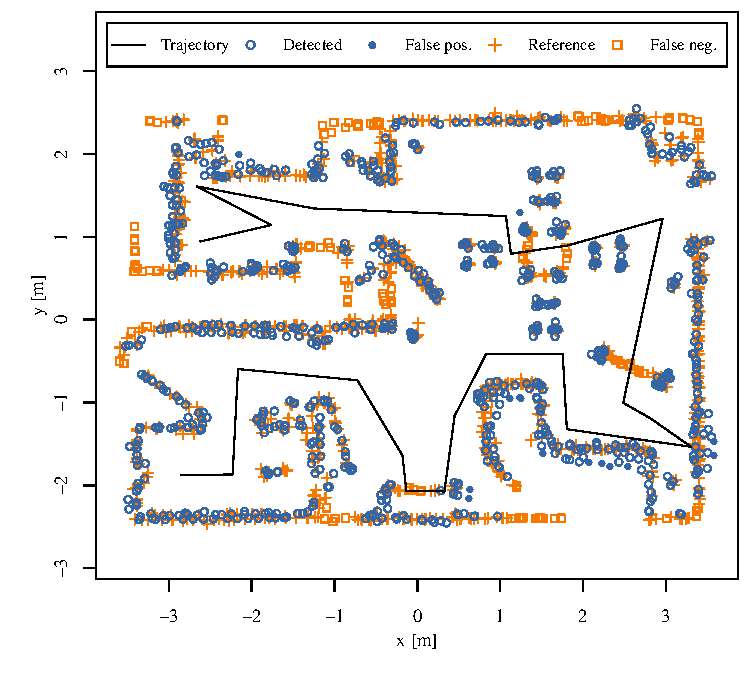
\includegraphics[width=0.975\textwidth]{results/simulation/apartment_overview.pdf}
  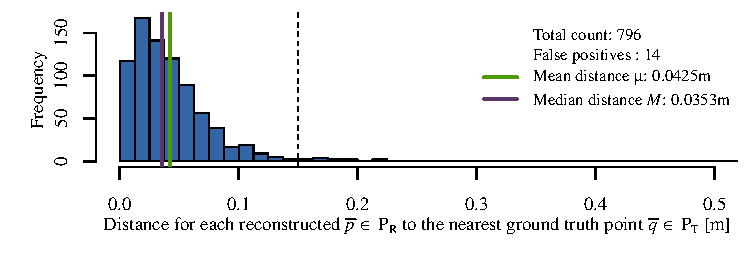
\includegraphics[width=0.975\textwidth]{results/simulation/apartment_histogram.pdf}
  \renewcommand{\arraystretch}{1.25}
  \begin{tabular}{l  l | l  l}
   Reconstructed count: & $796$ & Ground truth count: & $1150$ \\
   \hline
   False positives: & $14$ & True positive: & $782$ \\
   \hline
   $\nu_F$: & $1.76\%$ & $\nu_T$: & $68\%$ \\
   \hline
   $\mu$: & $0.0425 \,\mathrm{m}$ & $M$: & $0.0353 \,\mathrm{m}$ \\
   \hline
   $\mu_D$: & $0.594 \,\mathrm{m}$ & $M_D$: & $0.218 \,\mathrm{m}$ \\
   \hline
   Average time: & $24.28 \, \mathrm{ms}$ & Max. time:& $35.40 \, \mathrm{ms}$
  \end{tabular}
  \renewcommand{\arraystretch}{1}
 \end{center}
 \caption{Overall results for a simulated run in the apartment scene using the default parameters described above. See figure \ref{fig:floorplan} for the room layout.}
 \label{fig:simulation_result_apartment}
 \end{leftfullpage}
\end{figure}

\begin{figure}[p]
 \begin{fullpage}
 \begin{center}
  \textbf{Laboratory scene}\\
  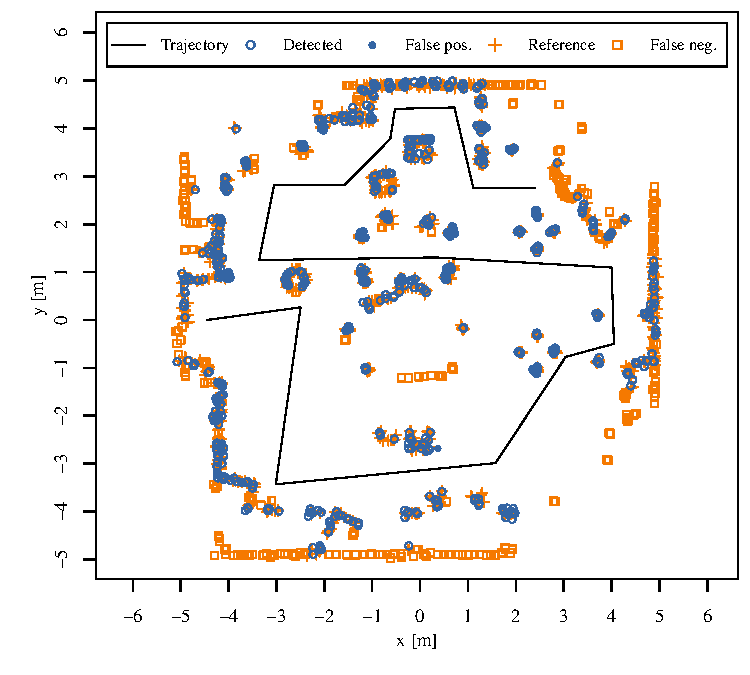
\includegraphics[width=0.975\textwidth]{results/simulation/laboratory_overview.pdf}
  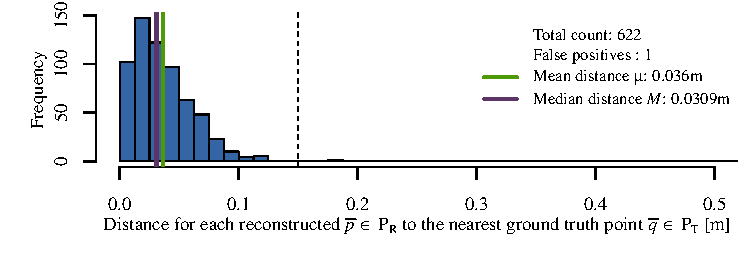
\includegraphics[width=0.975\textwidth]{results/simulation/laboratory_histogram.pdf}
  \renewcommand{\arraystretch}{1.25}
  \begin{tabular}{l  l | l  l}
   Reconstructed count: & $622$ & Ground truth count: & $1225$ \\
   \hline
   False positives: & $1$ & True positive: & $621$ \\
   \hline
   $\nu_F$: & $0.16\%$ & $\nu_T$: & $51\%$ \\
   \hline
   $\mu$: & $0.036 \,\mathrm{m}$ & $M$: & $0.0309 \,\mathrm{m}$ \\
   \hline
   $\mu_D$: & $0.769 \,\mathrm{m}$ & $M_D$: & $0.307 \,\mathrm{m}$ \\
   \hline
   Average time: & $16.39 \, \mathrm{ms}$ & Max. time:& $27.2 \, \mathrm{ms}$
  \end{tabular}
  \renewcommand{\arraystretch}{1}
 \end{center}
 \caption{Overall results for a simulated run in the laboratory scene using the default parameters described above. See figure \ref{fig:floorplan} for the room layout.}
 \label{fig:simulation_result_laboratory}
 \end{fullpage}
\end{figure}

%%%%%%%%%%% END DOUBLE PAGE %%%%%%%%%%%%%%%%

This section features a set of experiments in the environments described above and the corresponding results. First the overall results for both simulation and real-world tests are presented. Subsequent experiments seek to explore the impact of the error stack bias parameter $\tau$, the effects of coarse-to-fine refinement and the robustness against noise.

\subsection{Default parameters}

Unless noted differently, the following default parameters are used for both simulation and real-world tests:
\begin{description}
 \item[Input image:] $720 \times 96$ pixels, depression angle $\check \gamma = 0^\circ$, elevation angle $\hat \gamma = 30^\circ$, reduced elevation angle (region in which the depth is reconstructed) $\hat \gamma' = 10^\circ$.
 \item[Error stack calculation:] $32$ error stack layers (at $d = 0.04 \, \mathrm{m}$ $r_i$ ranges from $r_0 = \infty$ to $r_{31} \approx 0.15 \mathrm{m}$), error stack bias $\tau = 1$.
 \item[Coarse-to-fine refinement:] Search range $K = 2 \kappa + 1 = 8$; $3$ coarse-to-fine refinement steps.
 \item[Minimum error search:] $W_\vec{p}$ is a $3 \times 3$ binomial filter kernel, $\lambda = 1$, one refinement iteration.
 \item[Local environment map:] The standard deviation in depth direction is chosen as $\sigma_r = 0.01 \cdot (r^2 + 1 \, \mathrm{m}^2)$, the environment map density value threshold as $\eta = 40$.
\end{description}

\subsection{Simulated test run}

\paragraph{Experiment description:} In this experiment a test run with the default parameters (as given above) is conducted for each simulated environment. Runtime measurements are performed on an Intel\textregistered\ Atom\texttrademark\ N2600 dual core CPU running at $1{.}60 \, \mathrm{GHz}$ (the same model controlling the target robot) and covers both the depth reconstruction and the obstacle detection stage.

\paragraph{Results:} The results of this test run can be seen in figure \ref{fig:simulation_result_apartment} (apartment scene) and \ref{fig:simulation_result_laboratory} (laboratory scene), where \textit{false negative} obstacle points are defined as reference points $\vec q \in P_T$ with $\mathcal{D}(\vec q; P_R) > \chi$.


In the apartment scene, the algorithm creates multiple false positive obstacle points in the couch region and a single false positive point in the table region. On the other hand, all major obstacles are detected, including the table and chair legs. Most walls are detected. Relatively few obstacle points are detected for the brushed stainless steel refrigerator and the glass front of the stove (bottom right and top middle of the kitchen).

In the laboratory scene a single false positive obstacle point is found. Generally fewer obstacle points are detected (likely due to the size and higher sparsity of the room), yet all obstacles surrounding the trajectory in a distance of up to $1$ to $1.5 \,\mathrm{m}$ are detected. A notable exception is the checkerboard in the middle of the room.

During the simulation run it can be observed that the detection range is smaller for obstacles which lie in the direction of the focus of expansion or the focus of contraction, unless the corresponding objects have a prominent texture. For example at the end of the trajectory in the laboratory scene one can see that the (untextured) cylinders lying directly in front of the robot are not detected. With an average execution time of $24.28 \; \mathrm{ms}$ and $16.39 \; \mathrm{ms}$, respectively, real-time execution is possible on the target processor.

\subsection{Real-world test run}

\begin{figure}[t]
 \begin{center}
  \subbottom[Reconstructed obstacle points\label{fig:results_real1:a}]{
  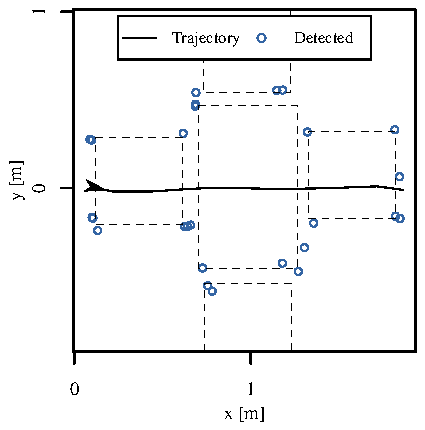
\includegraphics[width=0.475\textwidth]{results/real/obst5_furniture.pdf}
  }
  \subbottom[Local environment map\label{fig:results_real1:b}]{
  \raisebox{1.125cm}{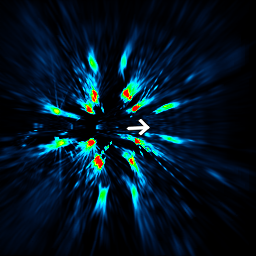
\includegraphics[width=0.385\textwidth]{results/real/obst5_map_ss.png}}
  }
  \subbottom[Depth reconstruction\label{fig:results_real1:c}]{
  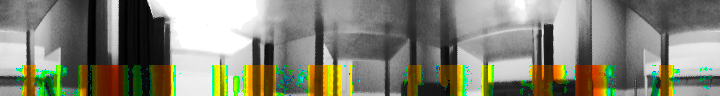
\includegraphics[width=0.85\textwidth]{results/real/obst5_depth_ss.png}
  }
  \subbottom[Artifacts introduced by tilting\label{fig:results_real1:d}]{
  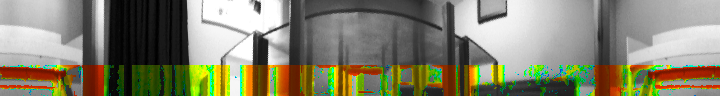
\includegraphics[width=0.85\textwidth]{results/real/obst5_depth2_ss.png}
  }
 \end{center}
 \caption{Test room dinner table results. (a) Obstacle points emitted during the test run and the corresponding trajectory (odometry data integration). The dashed lines depict the approximate position of the table and the four chairs (only shown for visualization and orientation purposes). (b) Local environment map. The arrow depicts the current robot position and orientation. (c) A snapshot of the depth reconstruction at the arrow position. Notice how the table legs are colored in yellow, orange and red depending on their distance. See figure \ref{fig:bias_depth_reconstruction} for details on the used color coding. (d) Artifacts in the depth reconstruction (note the red/near regions at the side and in the middle of the image) introduced by tilting the robot.}
 \label{fig:results_real1}
\end{figure}

\begin{figure}[t]
  \begin{center}
   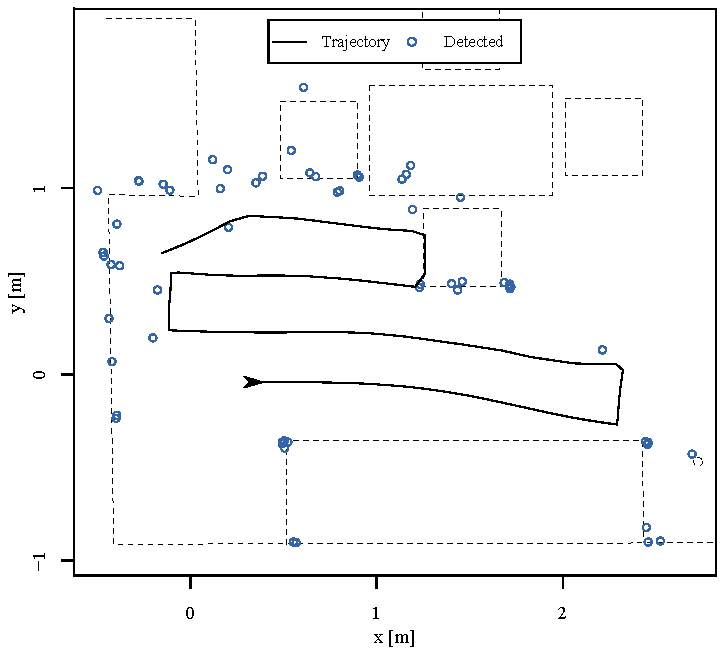
\includegraphics[width=0.975\textwidth]{results/real/obst6_furniture.pdf}
  \end{center}
  \caption{Test room results. Blue circles show obstacle points which were emitted during the test run, the straight line depicts the corresponding robot trajectory (odometry data integration). The dashed lines depict the approximate position of the furniture (table, four chairs, couch, sideboard) and the walls (only shown for visualization and orientation purposes). Note that the left wall is partially covered by a curtain.}
 \label{fig:results_real2}
\end{figure}

The results of two test runs in the test room environment described above can be seen in the figures \ref{fig:results_real1} and \ref{fig:results_real2}. Note that the environment map threshold $\eta$ (see section \ref{sec:obstacle_detection}) is doubled from $\eta = 40$ to $\eta = 80$ in order to increase the robustness against noise in exchange for a reduced detection range.

In the first test run, the robot drives a straight trajectory between the legs of the living room suite (see figure \ref{fig:results_real1:a}). The legs of chairs and tables are detected, although superimposed by relatively severe noise. In the depth reconstruction, the legs are correctly classified (figure \ref{fig:results_real1:c}), yet the depth of each leg spills onto background pixels. Correspondingly the probability distributions belonging to the table legs occupy relatively large regions in the local environment map (figure \ref{fig:results_real1:b}).

A false obstacle point is emitted at the end of the trajectory. At this position, the robot tilts/changes its elevation while driving over the edge of a carpet. Figure \ref{fig:results_real1:d} shows the corresponding artifacts in the depth map, which are responsible for the false positive obstacle point.

In the second test run, the legs of the couch (bottom region in figure \ref{fig:results_real2}) as well as the floor lamp to it's right are correctly detected. Correct obstacle points are also detected for the left wall which is partially covered by a curtain and two legs of the bottom chair. However, a large amount of false positive obstacle points is emitted in the top-left region of the trajectory.

\subsection{Error stack bias}

\begin{figure}[p]
 \begin{center}
  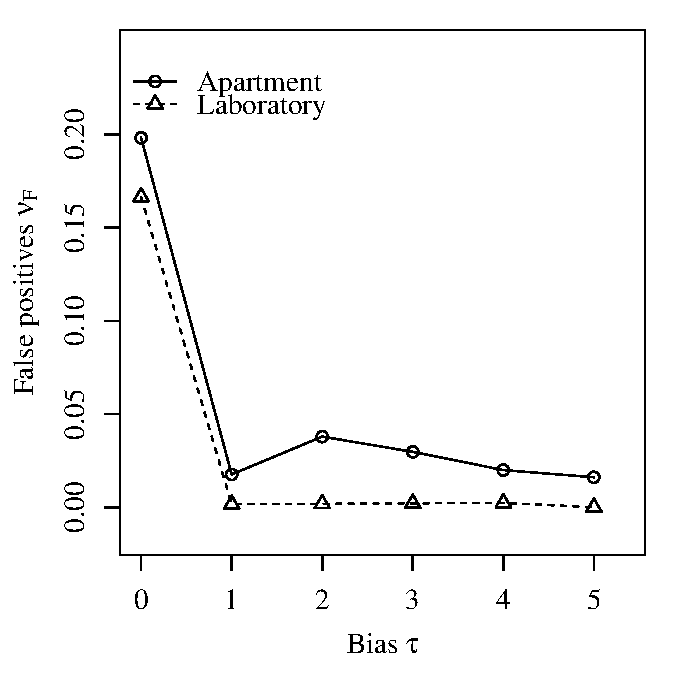
\includegraphics[width=0.44\textwidth]{results/bias/bias_mF.pdf}
  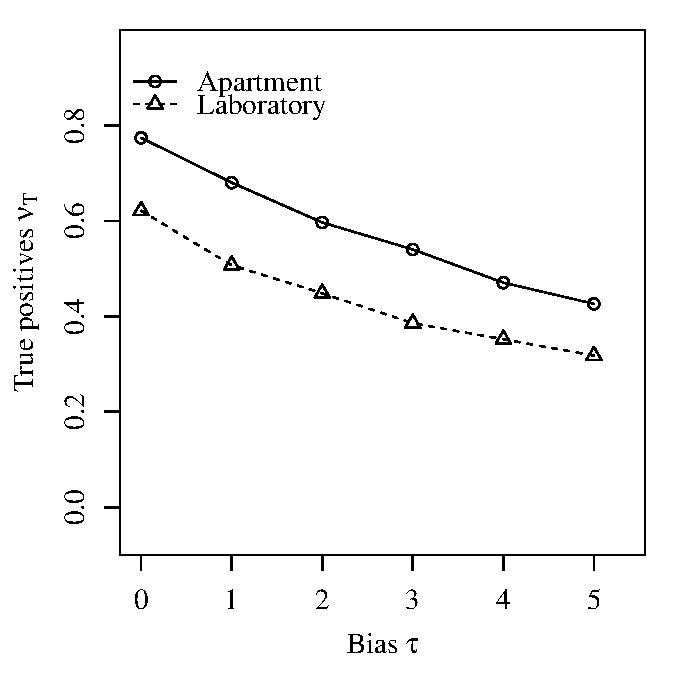
\includegraphics[width=0.44\textwidth]{results/bias/bias_mT.pdf}
  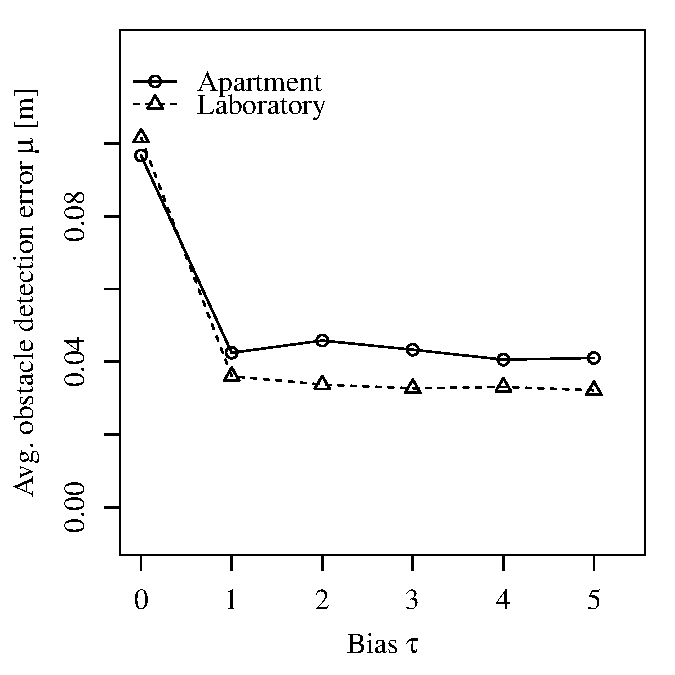
\includegraphics[width=0.44\textwidth]{results/bias/bias_meanDist.pdf}
  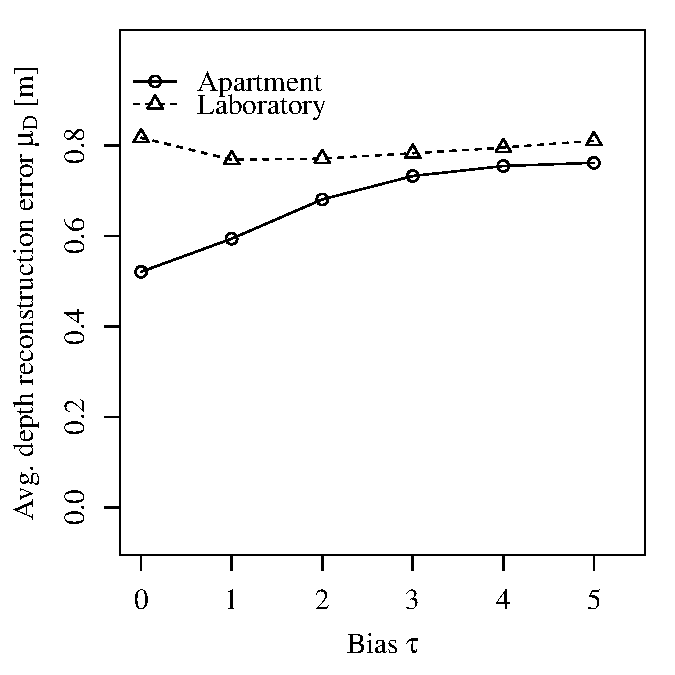
\includegraphics[width=0.44\textwidth]{results/bias/bias_avgNettoMean.pdf}
 \end{center}
 \caption{Results for varying the error stack bias $\tau$ for both the laboratory and the apartment scene.}
 \label{fig:results_bias}
\end{figure}

\begin{figure}[p]
\begin{center}
  \begin{tabular}{p{0.76\textwidth} p{0.085\textwidth}}
  \subbottom[$\tau = 0$]{
    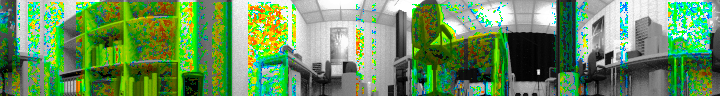
\includegraphics[width=0.75\textwidth]{results/bias/bias_off.png}
  }
  \subbottom[$\tau = 1$]{
    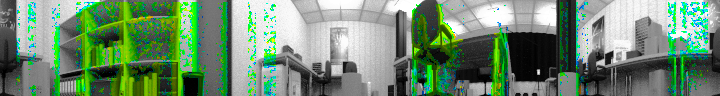
\includegraphics[width=0.75\textwidth]{results/bias/bias_on.png}
  }
  &
  \subbottom{
    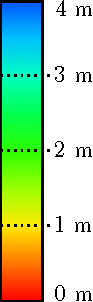
\includegraphics[width=0.084\textwidth]{media/depth_scale_vert.pdf}
  }
  \end{tabular}
\end{center}
\caption{Two depth reconstruction results for the laboratory scene for $\tau = 0$ and $\tau = 1$. For these particular images, the reduced elevation angle $\hat \gamma'$ was set to $\hat \gamma = 30^\circ$. Uncolored image regions either have a reconstructed distance larger than $4\,\mathrm{m}$ or were pruned in the coarse-to-fine refinement.}
\label{fig:bias_depth_reconstruction}
\end{figure}

\paragraph{Experiment description:} This test run measures the effect of the error stack bias parameter $\tau$ in the simulated environments (introduced in section \ref{sec:minimum_error_search}). The parameter $\tau$ is varied between $0$ and $5$. Due to restrictions in the optimized implementation only integral values are tested.

\paragraph{Results:} As shown in figure \ref{fig:results_bias}, nearly $\nicefrac{1}5$ of the reconstructed points are false positive for $\tau = 0$, in both laboratory scene and apartment scene. This number rapidly decreases as soon as $\tau \geq 1$. Yet a further increase in $\tau$ continuously decreases the count of reconstructed obstacle points as well as (at least in the apartment scene) the depth reconstruction error. Note how in the large laboratory room the depth reconstruction error decreases in the step from $\tau = 0$ to $\tau = 1$. The depth reconstruction result shown in figure \ref{fig:bias_depth_reconstruction} shows false classifications in unstructured areas of the input image for $\tau = 0$, which are eliminated for $\tau = 1$.

\subsection{Coarse-to-fine search}

\begin{figure}[t]
\begin{center}
 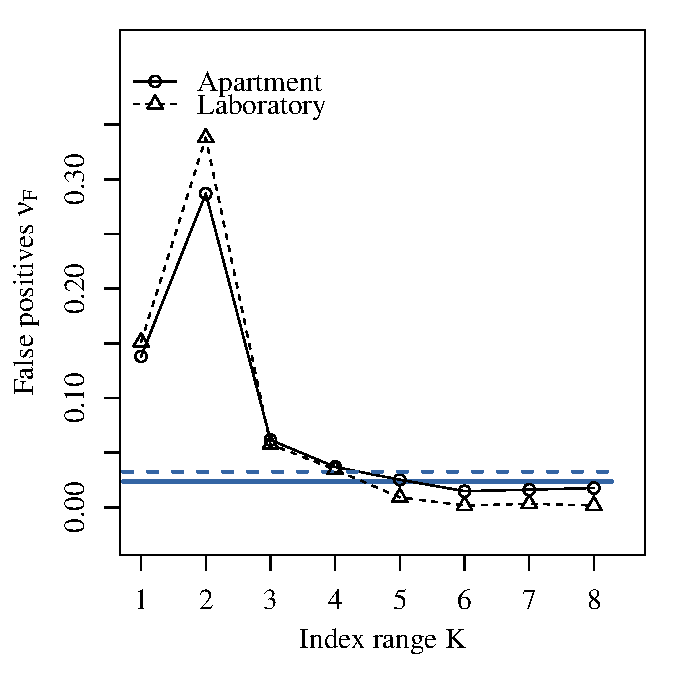
\includegraphics[width=0.475\textwidth]{results/index_range/idx_mF.pdf}
 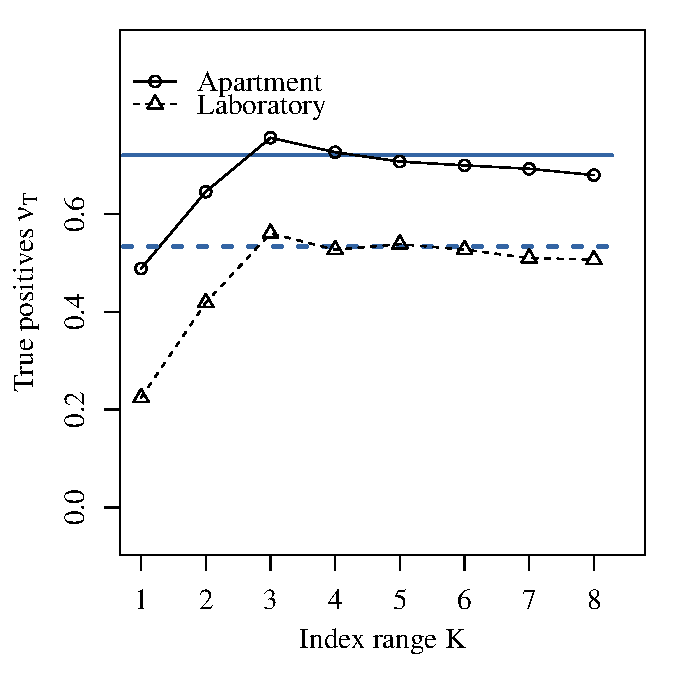
\includegraphics[width=0.475\textwidth]{results/index_range/idx_mT.pdf}
 %\includegraphics[width=0.475\textwidth]{results/index_range/idx_meanDist.pdf}
 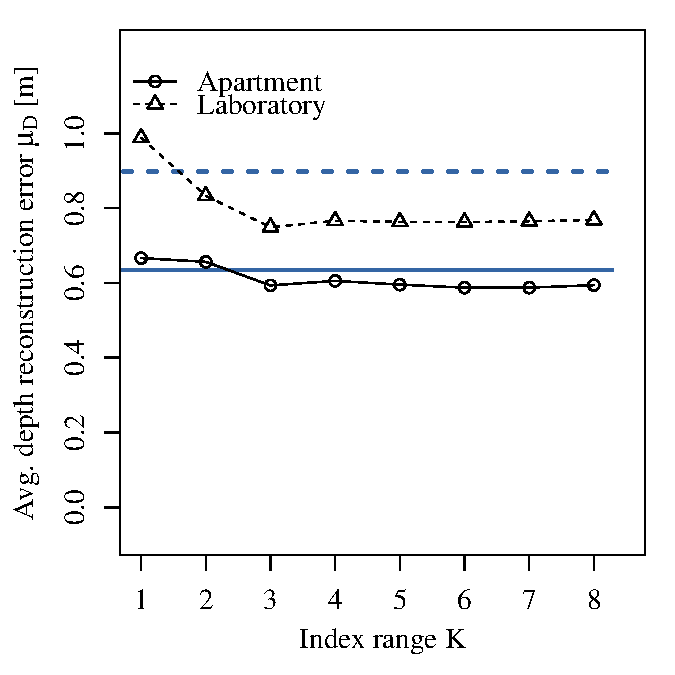
\includegraphics[width=0.475\textwidth]{results/index_range/idx_avgNettoMean.pdf}
 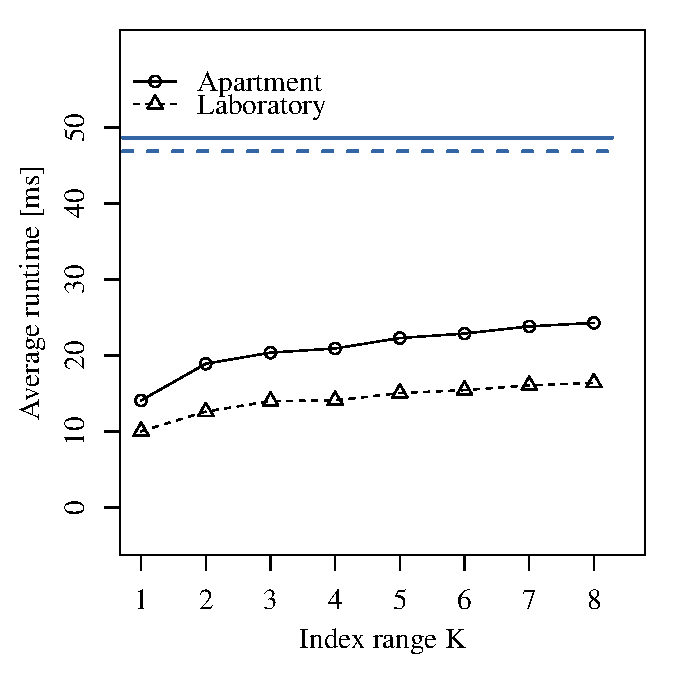
\includegraphics[width=0.475\textwidth]{results/index_range/idx_avgTime.pdf}
\end{center}
\caption{Results for varying index search range $K$ in both the apartment and the laboratory environment. The horizontal lines (blue) correspond to the result without coarse-to-fine refinement.}
\label{fig:results_index_range}
\end{figure}

\begin{figure}[t]
  \begin{center}
%  \subbottom[Reference run, no coarse-to-fine refinement]{
   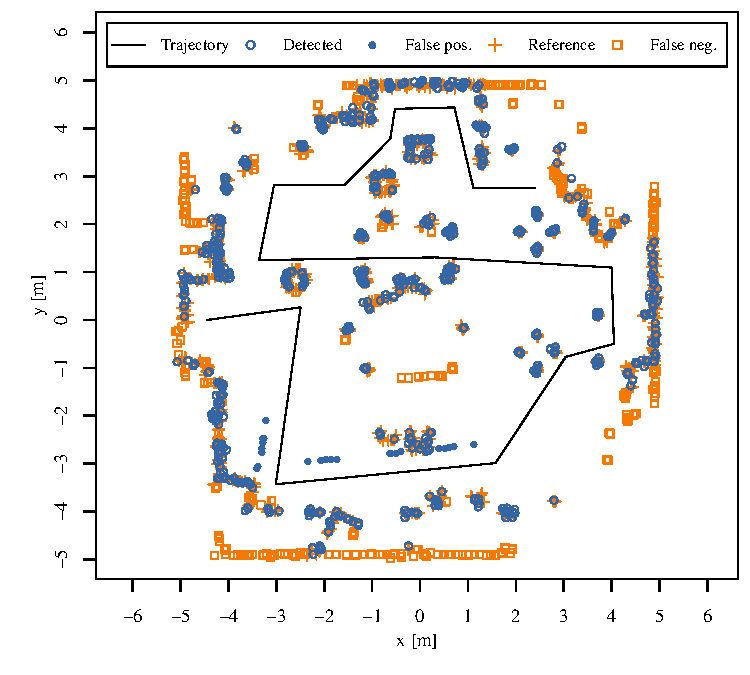
\includegraphics[width=0.975\textwidth]{results/index_range/overview_no_coarse_to_fine.pdf}
   %}
   %\subbottom[With coarse-to-fine refinement and $K = 8$]{
  % \includegraphics[width=0.75\textwidth]{results/index_range/overview_coarse_to_fine_8.pdf}
   %}
  \end{center}
  \caption{Obstacle detection performance in the simulated laboratory environment without coarse-to-fine refinement. Note the false positive points. See figure \ref{fig:floorplan} for a room plan and see figure \ref{fig:simulation_result_laboratory} for the run with coarse-to-fine refinement.}
  \label{fig:results_temporal_aliasing}
\end{figure}

\begin{figure}[t]
\begin{center}
  \subbottom[Without coarse-to-fine refinement]{
    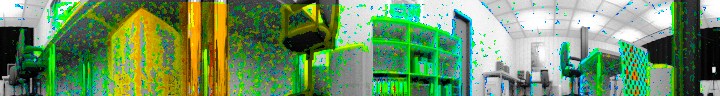
\includegraphics[width=0.75\textwidth]{results/index_range/index_range_off.png}
    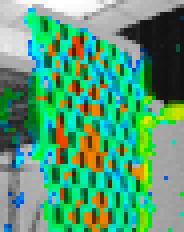
\includegraphics[width=0.08\textwidth]{results/index_range/small_no_coarse_to_fine.png}
  }
  \subbottom[Coarse-to-fine search, $K = 8$]{
    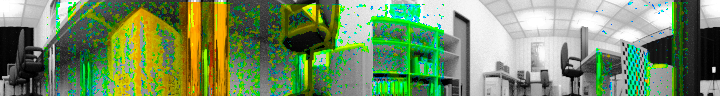
\includegraphics[width=0.75\textwidth]{results/index_range/index_range_on.png}
    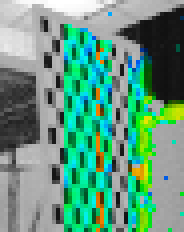
\includegraphics[width=0.08\textwidth]{results/index_range/small_coarse_to_fine.png}
  }
\end{center}
\caption{Two depth reconstruction results for the laboratory scene for the reference run (without coarse-to-fine refinement) (a) and with coarse-to-fine-search, $K = 8$ (b). The right images show the enlarged chess-board area. See figure \ref{fig:bias_depth_reconstruction} for details on the used color coding.}
\label{fig:coarse_to_fine_depth_reconstruction}
\end{figure}

\paragraph{Experiment description:} In this simulated test run the effects of the coarse-to-fine refinement on runtime and quality are to be measured.

The algorithm is executed in the apartment and laboratory test environments under different search range breadths $K \in \{1, \ldots, 8\}$. A reference run is performed in which coarse-to-fine refinement is disabled.

\paragraph{Results:} The result of the test runs is shown in figure \ref{fig:results_index_range}: One can see, that in comparison to the reference run, the depth reconstruction error $\mu_D$ is reduced for $K \geq 3$. The same is true for the false positive count $\nu_F$, yet a search range of $K = 6$ is required in order to perform considerably better in the apartment scene. For large search ranges the true positive count $\nu_T$ is slightly reduced compared to the reference value.

The runtime rises with increasing search range, yet even for $K = 8$ the total runtime is reduced by nearly $50\%$ compared to the reference run.

Figure \ref{fig:results_temporal_aliasing} shows detected and reference obstacle points as a global top-down map in the laboratory environment without coarse-to-fine refinement. In contrast to the result shown in figure \ref{fig:simulation_result_laboratory} (which had coarse-to-fine refinement enabled), false positive obstacle points are detected in the lower left region. This region features repeating patterns including a bookshelf and a chess board, see second laboratory snapshot example image in figure \ref{fig:sample_snapshots}. Figure \ref{fig:coarse_to_fine_depth_reconstruction} shows a snapshot of the depth reconstruction for that region, with both enabled and disabled coarse-to-fine refinement. One can see, that the coarse-to-fine refinement eliminates the artifacts in the depth map, which are suspected to cause the false positive obstacle points.

\subsection{Noise robustness}

\label{sec:noise}

\begin{figure}[p]
 \begin{center}
  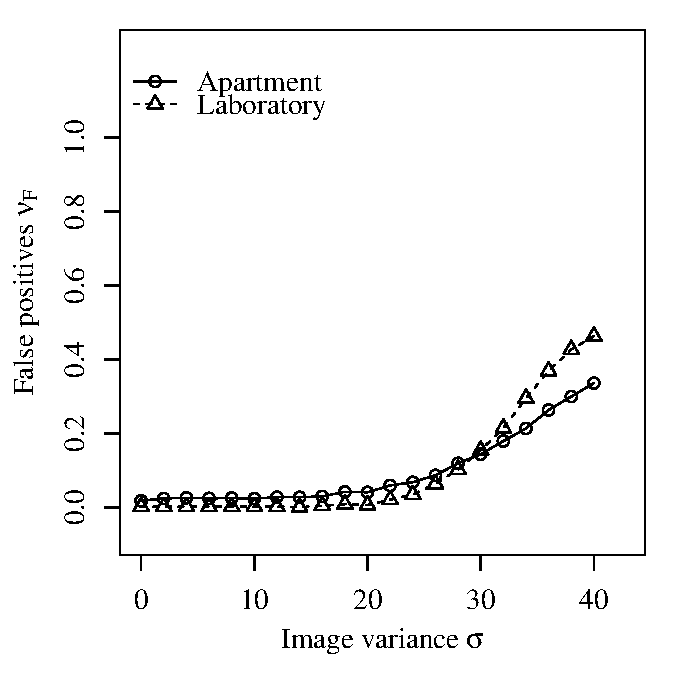
\includegraphics[width=0.475\textwidth]{results/noise/noise_image_mF.pdf}
  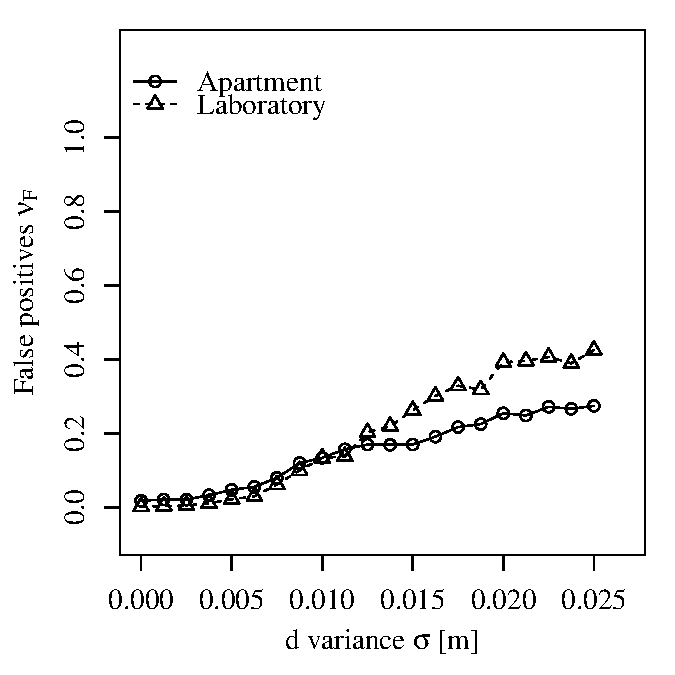
\includegraphics[width=0.475\textwidth]{results/noise/noise_d_mF.pdf}
  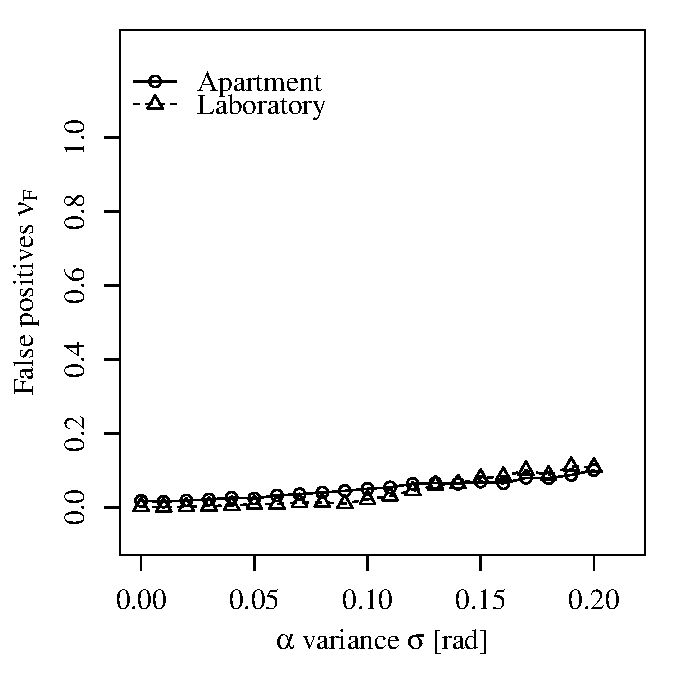
\includegraphics[width=0.475\textwidth]{results/noise/noise_alpha_mF.pdf}
  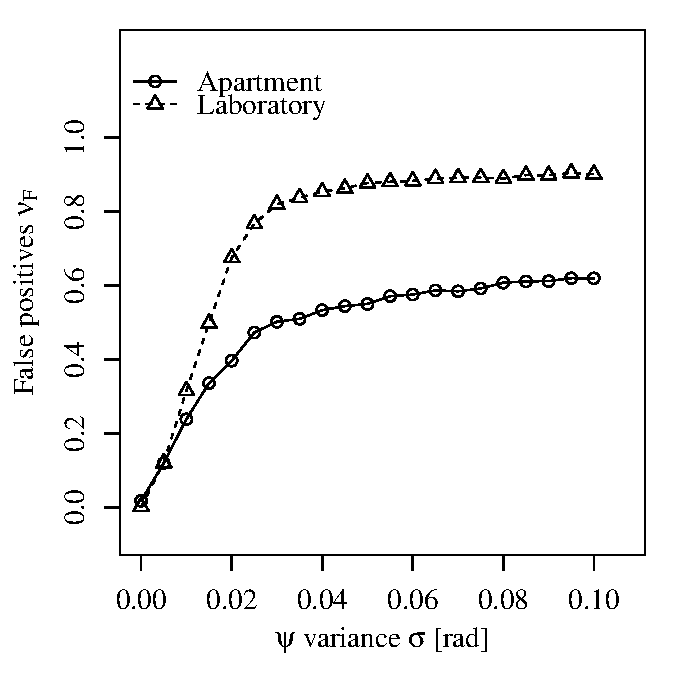
\includegraphics[width=0.475\textwidth]{results/noise/noise_psi_mF.pdf}
 \end{center}
 \caption{Impact of noise superimposed on the input images and the motion parameters on the relative false positive count $\nu_F$ for both the laboratory and the apartment scene.}
 \label{fig:results_noise}
\end{figure}

\begin{figure}[p]
 \begin{center}
  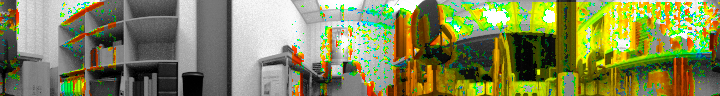
\includegraphics[width=0.85\textwidth]{results/noise/noise_depth_psi.png}
 \end{center}
 \caption{Depth reconstruction result for the laboratory scene showing artifacts introduced by a $0.0287$ radians ($1.64^\circ$) deviation of $\psi$. See figure \ref{fig:bias_depth_reconstruction} for details on the used color coding and the reference result.}
 \label{fig:noise_depth_reconstruction}
\end{figure}

\paragraph{Experiment description:} In this test, the impact of noisy input data is measured. The noise leads to violations of the assumptions made in section \ref{sec:assumptions}. The input data (motion parameters $d, \alpha$ and $\psi$, as well as the input image $\img{I}$) are superimposed by an additive Gaussian noise term with standard deviation $\sigma$. The noise is sampled independently at each data point/pixel.

The following (arbitrarily chosen) standard deviations are used: For $d$ (traveled distance) $\sigma$ is varied from $\sigma = 0 \, \mathrm{m}$ to $\sigma = 0.025 \, \mathrm{m}$ (the relative error at $d = 0.04$ ranges from $0\%$ to $62.5\%$). For $\alpha$ (motion direction) $\sigma$ is varied from $\sigma = 0 $ to $\sigma = 0.2$ radians (in degrees: $0^\circ$ to $11.46^\circ$). For $\psi$ (change in orientation) $\sigma$ is varied from $\sigma = 0 $ to $\sigma = 0.1$ (in degrees: $0^\circ$ to $5.73^\circ$). For the image $\img{I}$ the standard deviation is varied from $\sigma = 0$ to $\sigma = 40$ (relative deviation ranges from $0\%$ to $16\%$ for 8-bit intensity values). In all experiments $\sigma$ is varied in 20 steps.

\paragraph{Results:} The results presented in figure \ref{fig:results_noise} show that independent noise superimposed on the input image and the motion parameters $\alpha$ and $d$ only has a very subtle impact on the count of false positive obstacles until certain thresholds are reached: Image noise starts to effect the output noticeably at $\sigma \approx 20$ ($8\%$), noise in $d$ is is tolerable up to $\sigma \approx 0.005 \, \mathrm{m}$ ($12.5\%$) and noise in $\alpha$ has only little effect on the false positive count for deviations up to $\sigma \approx 0.1$ radians ($5.73^\circ$). However, even small deviations in the orientation change $\psi$ result in a high false positive count: Even a deviation of $0.02$ radians ($\approx 1^\circ$) causes almost every second reconstructed obstacle point to be false positive. See figure \ref{fig:noise_depth_reconstruction} for the impact of noisy $\psi$ on the depth reconstruction.

\chapter{Discussion and conclusion}

In this chapter the results from the previous chapter are discussed, followed by a brief conclusion and an outlook concerning future work.

\section{Discussion}

\subsection{Simulated test runs}

The results of the simulated test runs show that the algorithm presented in this thesis is capable of reconstructing obstacles from a time-series of of spherical panoramic images and fully fulfills the real-time constraints, typically requiring less than $30 \, \mathrm{ms}$ per snapshot on the target platform, an Intel\textregistered\ Atom\texttrademark\ N2600 dual core CPU running at $1{.}60 \, \mathrm{GHz}$.

As expected, the heuristic used in the depth reconstruction stage produces very coarse results: The mean depth reconstruction error ranges from $0.5$ to $0.8 \, \mathrm{m}$. However, the post-processing of the reconstructed landmark points in the local environment map increases the obstacle detection precision by an order of magnitude, allowing the algorithm to detect obstacle points with a median error of about $3 \, \mathrm{cm}$ and mean error of about $6 \, \mathrm{cm}$ if perfect odometry data is available.

The algorithm is unexpectedly robust concerning glossy surfaces, although these were explicitly excluded from the assumptions made in section \ref{sec:assumptions}: The stainless steel table legs in the laboratory scene are correctly detected, and while obstacle points are detected at the edges of the stainless steel refrigerator only, its glossiness does not cause any false positive obstacle points.

The false positive obstacle points in the apartment scene are believed to be caused on the one hand by the virtual camera moving too close to the obstacles ($< 0.15 \, \mathrm{m}$, which is smaller than the distance corresponding to the last flow template) and on the other hand by the error stack bias, which causes local minima belonging to larger distances to be preferred.

The algorithm works best if the obstacles are structured, allowing for a distinct global minimum in the error stack. Unstructured objects, for example the cylinders in the laboratory scene, are only detected at their edges. The algorithm is even capable of precisely reconstructing walls, as soon as those have some visible structure (like the tiled walls in the bathroom).

\subsection{Real-world test}

Earlier tests of the robot under laboratory conditions (results not shown here) have shown that the obstacle detection algorithm is capable of correctly detecting obstacles with no or only few false positives. The relatively poor performance under realistic test conditions is believed to be caused by the following factors:
\begin{description}
 \item[Noisy orientation change parameter $\psi$:] This may be caused by the odometry data not being captured synchronously with the snapshots. Especially when the robot is rotating, large deviations in $\psi$ become apparent.
 \item[Tilting and change in elevation:] In the test room, the edges of the carpet are especially problematic. While small tilt could be avoided by equipping the robot with some kind of mechanical suspension, tilt in critical quantity needs to be detected.
 \item[Unstructured environment:] The room is relatively sterile featuring only uniformly colored objects.
\end{description}

The spreading of the reconstructed depth seen in figure \ref{fig:results_real1:c} is partially assumed to be caused by occlusions and by the use of small space-invariant local error propagation matrices: There is no way for the depth reconstruction to decide which parts of the image are connected. Assuming that the uniformly colored background belongs to one of the chair/table legs is perfectly valid. This problem could only be solved by using global optical flow estimates \citep{totalVariation,flowchapter05} which are most likely not suitable for real-time execution on the robot.

However, the extreme impact of noise in $\psi$ as shown in the corresponding experiment provides evidence that hardening the algorithm against this problem will also increase its real-world performance.

\subsection{Detailed experiments}

\paragraph{Error stack bias:} The error stack bias $\tau$ proves to be mandatory for the obstacle-detection algorithm and behaves as intended: The bias promotes landmarks in regions with no visible structure to be classified as far-distance landmarks, which will then be ignored in later stages. The choice of $\tau$ turns out to be uncritical as long as chosen larger than zero.

\paragraph{Coarse to fine search:} The results show that the coarse-to-fine refinement eliminates most artifacts resulting from temporal aliasing in regions with repeating patterns. Depending on the environment this can lead to a significant decrease in the count of false-positive obstacle points. Moreover, the pruning and the limited search range introduced along with the coarse-to-fine refinement reduce the total runtime by almost $50\%$. When comparing depth-reconstruction results, the pruning sometimes appears to be oversensitive, yet the data show that the decrease in the count of true positive obstacle points is negligible.

\paragraph{Noise:} Noise in the orientation change parameter $\psi$ proves to render the depth reconstruction result useless. This can partially be explained by the two following effects:
\begin{description}
\item[Reciprocal shift-to-depth function:] As derived in appendix \ref{proof:max_horz_shift}, a horizontal pixel shift $\Delta x$ between two projected landmark points $\vec p_1$ and $\vec p_2$ can approximately be transformed into a landmark distance:
\begin{align*}
  r &\approx \frac{w}{2 \pi} \cdot \frac{d}{\Delta x} \; .
\end{align*}
If additive noise is superimposed on small $\Delta x$, this results in a large change in $r$.
\item[Forward search along flow lines:] Another problem concerns the fact that the minimum error search along a flow line --- as performed in the error stack calculation --- is always a forward search. Noise in $\psi$ can cause $\img{CV}$ and $\img{SS}$ to be aligned in such a way that the actual global minimum has already passed (at least in one half of $\img{CV}$). Due to the forward search only the next local minimum can be used.
\end{description}

\section{Conclusion}

The optimizations presented in this thesis allow to perform obstacle detection based on a time-series of spherical panoramic images while fulfilling the real-time constraint present on the used robot. The results from the simulated test environments prove that the general algorithm is working as intended and the introduced measures allow to verify how changes in the algorithm will effect the overall performance. Yet in order to be usable in arbitrary domestic in-door environments, the reliability of the algorithm needs to be increased.

\section{Outlook}

The following compilation enumerates some future research topics which are either hoped to resolve current issues, to further optimize the runtime requirements, or to be interesting from a scientific point of view.

\paragraph{Hardening against noise in $\psi$:} As the odometry data obtained from the robot turned out to be far from perfect, the algorithm needs to be hardened against noise, especially in the orientation change parameter $\psi$. This problem could be solved in software by either using an image compass or by repeating the depth reconstruction algorithm (up to the minimum error search) for varying $\psi$ and selecting the ``best'' result. The criteria for this choice need to be developed.

\paragraph{Optimization of the landmark selection:} Currently all reconstructed landmarks originating from a single column are inserted into the local obstacle map with equal weight. A further optimization would be to select the prevalent distances from the column and to insert fewer, but weighted landmark points into the obstacle map. The selection could for example be performed by one-dimensional $k$-means.

\paragraph{Combination of multiple depth maps:} Another possible extension would be to reconstruct the depth for multiple snapshots relative to a single current view. The resulting depth maps can then be combined into a single result by calculating the mean distance and pruning regions with high variance in the results. Yet this approach might prove to be difficult due to accumulating odometry errors.

\paragraph{Comparison to existing approaches:} The results of this algorithm need to be compared to competing approaches, including feature based sparse optical flow as introduced in section \ref{sec:existing_solutions}.

\paragraph{Navigation:} It would also be interesting to explore whether the local environment maps and the reconstructed obstacle points can be used for navigation.

\paragraph{GPU implementation:} As the depth reconstruction is intrinsically parallel in every pixel (each pixel only depends on its direct neighbors), a GPU implementation using either the compute languages OpenCL or CUDA, or a GPGPU implementation using OpenGL (or to some degree even OpenGL ES) is believed to be viable.

\paragraph{Color images:} It would be interesting to test the algorithm with color images as input. The availability of color increases the input dimensionality and is expected to allow for fewer ambiguities in the minimum error search.


\begin{appendix}
\chapter{Derivations and proofs}

This appendix contains derivations and proofs for some of the statements made throughout the thesis. A note on notation: In order to shorten some equations, $\cos(\alpha)$ and $\sin(\alpha)$ are replaced by the shorter $c_\alpha$ and $s_\alpha$.

\section{Probabilistic landmark model}

\subsection{Covariance matrix transformation}

\label{proof:covariance_matrix_transformation}

\begin{figure}[t]
 \begin{center}
  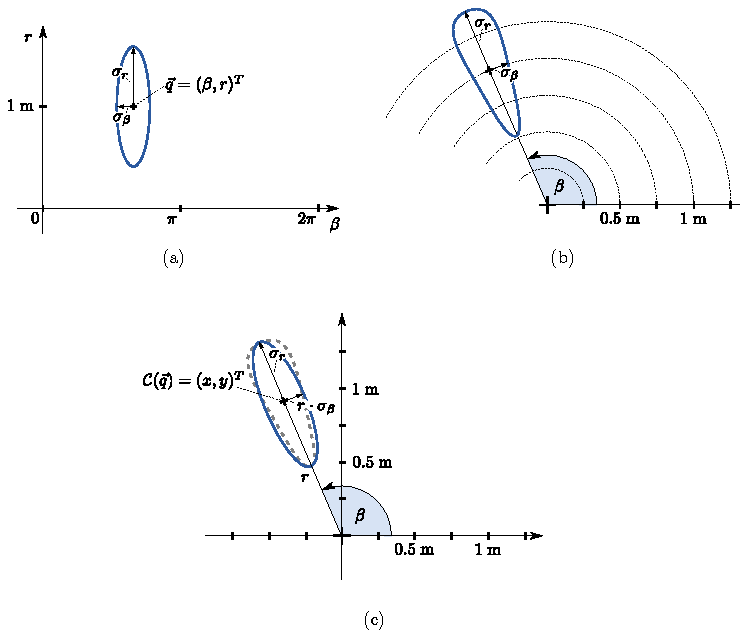
\includegraphics[width=0.975\textwidth]{media/gauss_cartesian.pdf}
 \end{center}
 \caption{Idea of the covariance matrix transformation from polar coordinates to Cartesian coordinates. (a) Shows a contour of the original Gaussian distribution in polar space. (b) Shows the same distribution drawn in a polar coordinate system. Note how the distribution is distorted. (c) Shows the approximated Gaussian distribution in a Cartesian coordinate system. The distortion present in (b) is discarded. The angular variance $\sigma_\beta$ is transformed to Cartesian coordinates by multiplication with the radius $r$. The covariance matrix of the Cartesian distribution is then calculated by rotating the Eigenraum of the original covariance matrix.}
 \label{fig:gauss_cartesian}
\end{figure}

The covariance matrix of the Gaussian distribution for polar coordinates $\vec q = (\beta, r)^T$ was given in equation \ref{eqn:gaussian_polar} as
\begin{equation*}
  \vec q_R \sim \mathcal{N}\left(\vec q_E, \Sigma(\vec q_E) \right) \text{ where } \Sigma(\beta, r) := \begmat \sigma_\beta^2 & 0 \\ 0 & \sigma_r^2 \finmat \; .
\end{equation*}
This distribution can be estimated by a Gaussian distribution in Cartesian space (see figure \ref{fig:gauss_cartesian} for an overview). Note that the estimation introduces a small bias towards smaller distances. The magnitude of this bias depends on the ratio of $\sigma_\beta$ to $\sigma_r$. The estimation is performed by choosing a covariance matrix $\Sigma_{\mathcal{C}}$ with Eigenvectors pointing in radial direction and the corresponding orthogonal direction. The Eigenvectors $\vec v_r, \vec v_\beta$ of $\Sigma_{\mathcal{C}}$ should hence have the following form:
\begin{align*}
 \vec v_r &= \begmat c_\beta \\ s_\beta \finmat & \vec v_\beta &= \begmat -s_\beta \\ c_\beta \finmat^T
\end{align*}
The Eigenvalues of a Covariance matrix correspond to the squared standard deviations of the elementary distributions:
\begin{align*}
 \lambda_r &= \sigma_r^2 &
 \lambda_\beta &= (r \cdot \sigma_\beta)^2
\end{align*}
The angular standard deviation needs to be multiplied with $r$, as in Cartesian coordinates the length of the underlying circle segment scales with the radius. The desired $\Sigma_{\mathcal{C}} = \begmat a & b \\ b & c \finmat$ can now be described by the following equations:
\begin{align*}
	 \Sigma_{\mathcal{C}} \cdot \vec v_r = \begmat a & b \\ b & c \finmat \begmat  c_\beta \\  s_\beta \finmat &= \lambda_r \begmat c_\beta \\  s_\beta \finmat \\
	 \Sigma_{\mathcal{C}} \cdot \vec v_\beta = \begmat a & b \\ b & c \finmat \begmat -s_\beta \\  c_\beta \finmat &= \lambda_\beta \begmat -s_\beta \\ c_\beta \finmat
\end{align*}
Solving the equations for $b$ yields:
\begin{align*}
	b &= \frac{(\lambda_r - a)  \cdot c_\beta}{s_\beta}
	= \frac{(\lambda_r - c)  \cdot s_\beta}{c_\beta}
	= \frac{(a - \lambda_\beta) \cdot s_ \beta}{c_\beta}
	= \frac{(c - \lambda_\beta) \cdot c_\beta}{s_\beta}
\end{align*}
Solve these equalities for $a$, $c$ and $b$:
\begin{align*}
	a &= \lambda_r c_\beta^2 + \lambda_\beta s_\beta^2 \\
	c &= \lambda_r s_\beta^2 + \lambda_\beta c_\beta^2 \\
	b &= \left(\lambda_r (1 - c_\beta^2) + \lambda_\beta s_\beta^2 \right) \frac{c_\beta}{s_\beta}
	  = \left(\lambda_r c_\beta^2 + \lambda_\beta (s_\beta^2 - 1) \right) \frac{s_\beta}{c_\beta}
	  = c_\beta s_\beta (\lambda_r - \lambda_\beta)
\end{align*}
The Cartesian approximate of the polar covariance matrix is thus given as:
\begin{align*}
	\Sigma_{\mathcal{C}}(\beta, r) &= \begmat
	    (\sigma_r c_\beta)^2 + (r \sigma_\beta s_\beta)^2 & c_\beta s_\beta (\sigma_r^2 - (r \sigma_\beta)^2) \\
	    c_\beta s_\beta (\sigma_r^2 - (r \sigma_\beta)^2) & (\sigma_r s_\beta)^2 + (r \sigma_\beta c_\beta)^2
	\finmat
\end{align*}


\subsection{Derivation of $\sigma_\beta$ for adjacent Gaussian distributions}

\label{proof:sigma_beta}

The angular variance $\sigma_\beta$ used in equation \ref{eqn:sigma_beta} is derived by demanding that the sum two adjacent Gaussian distributions ($\mu_1 = \mu_2 + \Delta \beta$) nearly forms a uniform distribution in the interval $[\mu_1, \mu_2]$ as shown in figure \ref{fig:sigma_beta}. The variance can be derived as a solution to the following more general problem:

Given the sum of two (one dimensional) Gaussian distributions with means $\mu_1$ and $\mu_2$ (where $\zeta := \mu_2 - \mu_1$) and a common variance $\sigma$:
  $$f(x) = \mathcal{N}(x \mid \mu_1, \sigma) + \mathcal{N}(x \mid \mu_2, \sigma)$$
Goal: Find $\sigma$ such that second derivative of $f(x)$ at $x = \mu_1 + \nicefrac{\zeta}2$ equals zero:
  $$\left. \frac{\partial f}{\partial x^2} \right|_{x = \mu_1 + \nicefrac{\zeta}2} \overset{!}= 0$$
By shifting $\mu_1 + \nicefrac{\zeta}2$ to the origin, the equation can be rewritten as:
  $$
  \left. \frac{\partial f\left(x - \mu_1 - \nicefrac{\zeta}2\right)}{\partial x^2} \right|_{x = 0} = \left. \frac{\partial}{\partial x^2} \; \left( \mathcal{N}\left(x \mid -\nicefrac{\zeta}2, \sigma\right) + \mathcal{N}\left(x \mid \nicefrac{\zeta}2, \sigma\right) \right) \right|_{x = 0} \overset{!}= 0$$
Derivation and evaluation at $x = 0$ yield ($\alpha$ represents all omitted normalization and constant factors):
  $$\left. \frac{\partial}{\partial x^2} \; \left( \mathcal{N}\left(x \mid -\nicefrac{\zeta}2, \sigma\right) + \mathcal{N}\left(x \mid \nicefrac{\zeta}2, \sigma\right) \right) \right|_{x = 0} = \alpha \cdot \frac{\exp\left(-\frac{\zeta^2}{8 \, \sigma^2}\right)}{\sigma^5} \left( -4\,\sigma^2+\zeta^2 \right) \overset{!}= 0$$
The solution for $\sigma$ is then given as
  $$\sigma = \pm \frac{\zeta}2 \; .$$
Setting $\zeta = \Delta \beta$ yields the term used in equation \ref{eqn:sigma_beta}.

\section{Motion field equation}

\subsection{Substitution of $r$ and $d$}

\label{proof:flow_subst}

The parameters $r$ and $d$ of equation \ref{eqn:motion_field_vector} are redundant and can be substituted by a single parameter $\rho := \frac{d}{r}$.

\begin{proof}
Equation \ref{eqn:motion_field_vector} was given as
\begin{align*}
\vec u(\vec p; T(d, \psi, \alpha), r) &= \begmat
  \beta' - \beta \\
  \gamma' - \gamma
\finmat \; .
\end{align*}
Expand the equation as defined in \ref{eqn:project}, \ref{eqn:unproject} and \ref{eqn:transform}. As $\atantwo(y, x)$ only selects the sign of the result depending on the quadrant of the input vector, $\atantwo(y, x)$ is substituted by $\arctan(\nicefrac{y}x)$ in this proof.
\begin{align*}
\beta' &= \arctan
    \left(
      \frac{
	- r s_{\psi} c_\beta + r c_{\psi} s_\beta + d s_{\alpha}
      }{
          r c_{\psi} c_\beta + r s_{\psi} s_\beta + d c_{\alpha}
      }
    \right) \\
    &= \arctan
    \left(
      \frac{
	  r \cdot (-s_{\psi} c_\beta + c_{\psi} s_\beta + \rho s_{\alpha} )
      }{
          r \cdot ( c_{\psi} c_\beta + s_{\psi} s_\beta + \rho c_{\alpha} )
      }
    \right) \\
    &= \arctan
    \left(
      \frac{
	  -s_{\psi} c_\beta + c_{\psi} s_\beta + \rho s_{\alpha}
      }{
          c_{\psi} c_\beta + s_{\psi} s_\beta + \rho c_{\alpha}
      }
    \right) \\
\gamma' &= \arctan
    \left(
      \frac{
	r \cdot \tan(\gamma)
      }{
	\sqrt{
	  (  r c_{\psi} c_\beta + r s_{\psi} s_\beta + d c_{\alpha})^{2} +
	  (- r s_{\psi} c_\beta + r c_{\psi} s_\beta + d s_{\alpha})^{2}}
      }
    \right) \\
    &= \arctan
    \left(
      \frac{
	r \cdot \tan(\gamma)
      }{
	r \cdot \sqrt{
	  (  c_{\psi} c_\beta + s_{\psi} s_\beta + \rho c_{\alpha})^{2} +
	  (- s_{\psi} c_\beta + c_{\psi} s_\beta + \rho s_{\alpha})^{2}}
      }
    \right)\\
    &= \arctan
    \left(
      \frac{
	\tan(\gamma)
      }{
	\sqrt{
	  (  c_{\psi} c_\beta + s_{\psi} s_\beta + \rho c_{\alpha})^{2} +
	  (- s_{\psi} c_\beta + c_{\psi} s_\beta + \rho s_{\alpha})^{2}}
      }
    \right)
\end{align*}
\end{proof}

\subsection{Rotational motion elimination}

\label{proof:rot_motion_elim}

It was stated in equation \ref{eqn:rot_motion_elim}:
  $$\vec u(\vec p; \psi, \alpha, \rho) = \vec u(\vec p - (\psi + \alpha, 0)^T; 0, 0, \rho) - (\psi, 0)^T$$

\begin{proof}
Prove the equation in two steps using the results derived in the previous section \ref{proof:flow_subst}:
\begin{enumerate}[1.]
 \item It holds $\vec u(\vec p; \alpha, \psi, \rho) = \vec u(\vec p - (\psi, 0)^T; \alpha, 0, \rho) - (\psi, 0)^T$. Apply the addition theorems:
 \begin{align*}
\beta'(\beta, \psi) &= \arctan
    \left(
      \frac{
	  -s_{\psi} c_\beta + c_{\psi} s_\beta + \rho s_{\alpha}
      }{
          c_{\psi} c_\beta + s_{\psi} s_\beta + \rho c_{\alpha}
      }
    \right) & \\
    &= \arctan\left(
      \frac{
	  \sin(\beta - \psi) + \rho s_{\alpha}
      }{
          \cos(\beta - \psi) + \rho c_{\alpha}
      }
    \right) \\
    &= \beta'(\beta - \psi, 0) \\
\gamma'(\beta, \psi) &= \arctan
    \left(
      \frac{
	\tan(\gamma)
      }{
	\sqrt{
	  (  c_{\psi} c_\beta + s_{\psi} s_\beta + \rho c_{\alpha})^{2} +
	  (- s_{\psi} c_\beta + c_{\psi} s_\beta + \rho s_{\alpha})^{2}}
      }
    \right) \\
    &= \arctan
    \left(
      \frac{
	r \cdot \tan(\gamma)
      }{
	r \cdot \sqrt{
	  (  \cos(\beta - \psi) + \rho c_{\alpha} )^{2} +
	  (  \sin(\beta - \psi) + \rho s_{\alpha})^{2}}
      }
    \right)\\
    &= \gamma'(\beta - \psi, 0)
\end{align*}
Plug these results into the definition of $\vec u$:
\begin{align}
\begin{aligned}
  \vec u(\vec p; \psi, \alpha, \rho) &=
  \begmat
    \beta'(\beta, \psi) - \beta \\
    \gamma'(\beta, \psi) - \gamma
  \finmat \\
  &= \begmat
    \beta'(\beta - \psi, 0) - \beta + \psi \\
    \gamma'(\beta - \psi, 0) - \gamma \\
  \finmat \\
  &= \vec u(\vec p - (\psi, 0)^T; \alpha, 0, \rho) - (\psi, 0)^T
\end{aligned}
\label{eqn:flow_prf1}
\end{align}
  \item It holds $\vec u(\vec p; \alpha, 0, \rho) = \vec u(\vec p - (\alpha, 0)^T; 0, 0, \rho)$. Expand the argument of the arctangent in $\beta'(\beta + \alpha, \alpha)$ using the addition theorems and reorder:
\begin{align*}
 \beta'(\beta - \alpha, \alpha) &{\overset{\phantom{\text{Rot. Mat.}\;}}=} \arctan
    \left(
      \frac{
	  \sin(\beta - \alpha) + \rho s_{\alpha}
      }{
          \cos(\beta - \alpha) + \rho c_{\alpha}
      }
    \right) \\
    &{\overset{\phantom{\text{Rot. Mat.}\;}}=} \arctan
    \left(
      \frac{
	  c_\alpha s_\beta - s_\alpha (c_\beta + \rho)
      }{
	  s_\alpha s_\beta + c_\alpha (c_\beta + \rho)
      }
    \right) \\
    &{\overset{\text{Rot. Mat.}\;}=} \arctan
    \left(
      \frac{
	  s_\beta
      }{
	  c_\beta + \rho
      }
    \right) + \alpha \\
    &{\overset{\phantom{\text{Rot. Mat.}\;}}=} \beta'(\beta, 0) - \alpha
\end{align*}
Analogously it holds for $\gamma'(\beta - \alpha, \alpha)$:
\begin{align*}
  \gamma'(\beta - \alpha, \alpha) &= \arctan
    \left(
      \frac{
	r \cdot \tan(\gamma)
      }{
	r \cdot \sqrt{
	  (  \cos(\beta - \alpha) + \rho c_{\alpha} )^{2} +
	  (  \sin(\beta - \alpha) + \rho s_{\alpha})^{2}}
      }
    \right) \\
    &= \arctan
    \left(
      \frac{
	r \cdot \tan(\gamma)
      }{
	r \cdot \sqrt{
	  (  s_\alpha s_\beta + c_\alpha (c_\beta + \rho) )^{2} +
	  (  c_\alpha s_\beta - s_\alpha (c_\beta + \rho) )^{2}}
      }
    \right) \\
    &= \arctan
    \left(
      \frac{
	r \cdot \tan(\gamma)
      }{
	r \cdot \sqrt{
	  (  c_\beta + \rho )^{2} +
	  (  s_\beta )^{2}}
      }
    \right) \\
    &= \gamma'(\beta, 0)
\end{align*}
Plug these results into the definition of $\vec u$:
\begin{align}
\begin{aligned}
\vec u(\vec p - (\alpha, 0)^T; 0, 0, \rho) &= \begmat
    \beta'(\beta - \alpha, \alpha) - \beta + \alpha \\
    \gamma'(\beta - \alpha, \alpha)
  \finmat \\
  &= \begmat
    \beta'(\beta, 0) - \beta \\
    \gamma'(\beta, 0)
  \finmat \\
  &= \vec u(\vec p; \alpha, 0, \rho)
\end{aligned}
\label{eqn:flow_prf2}
\end{align}
\end{enumerate}
Combining the results from equations \ref{eqn:flow_prf1} and \ref{eqn:flow_prf2} yields the desired equation.
\end{proof}

\subsection{Maximum horizontal shift}

\label{proof:max_horz_shift}

\begin{figure}[htb]
\begin{center}
 \subbottom[\label{fig:max_horz_shift}]{
 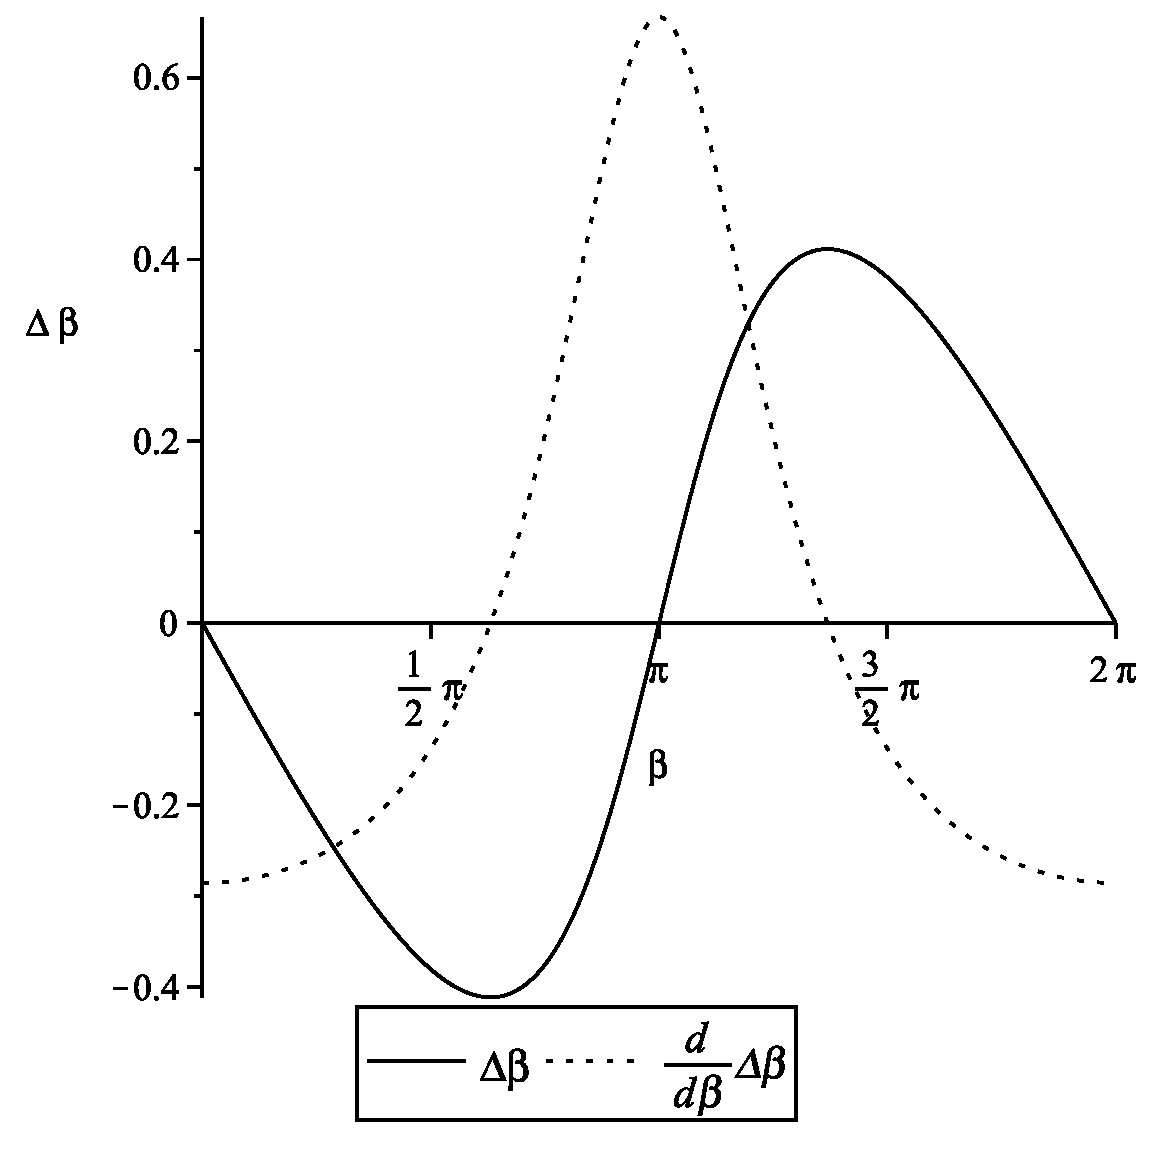
\includegraphics[width=0.475\textwidth]{media/max_horz_shift.pdf}}
 \subbottom[\label{fig:horz_shift_comparison}]{
 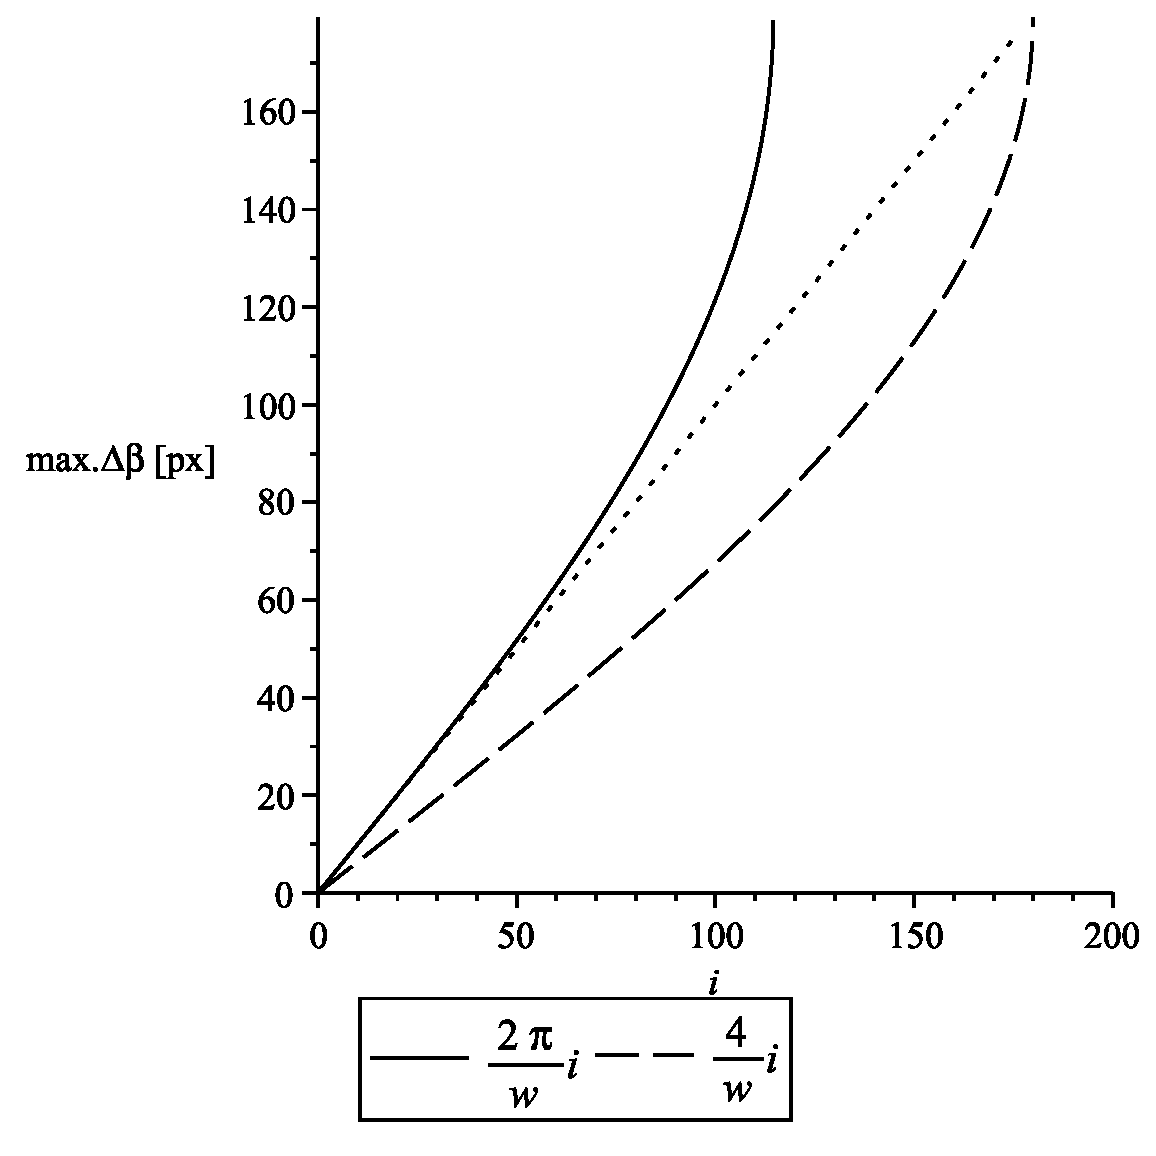
\includegraphics[width=0.475\textwidth]{media/horz_shift_comparison.pdf}}
\end{center}
\caption{(a) Plot of $\Delta \beta(\beta)$ and its derivative for $\rho = 0.4$. (b) A plot of the horizontal shift in pixels at $\hat \beta$ for both approximations presented below. The image width was set to $w = 720$. The dotted line represents the aimed-at behavior as achieved by the analytical solution.}
\end{figure}

In section \ref{sec:index_to_depth} the formula $\rho_i = \frac{2\pi}{w} \cdot i$ was introduced, which approximately ensures the horizontal motion field shift $\Delta \beta(\beta) = \beta'(\beta) - \beta$ to be smaller than one pixel per step for $0 \leq \rho \ll 1$.

\begin{derivation}
The shift in horizontal direction $\Delta \beta(\beta)$ is given as:
  $$\Delta \beta(\beta) = \beta'(\beta) - \beta = \atantwo \left(\sin(\beta), \cos(\beta) + \rho \right) - \beta$$
The extrema of this function can be found by calculating the first derivative and equating it with zero:
\begin{align*}
   \frac{\mathrm{d}}{\mathrm{d} \beta} \, \Delta \beta(\beta)&= \frac{\mathrm{d}}{\mathrm{d}\beta} \left( \atantwo \left(\sin(\beta), \cos(\beta) + \rho\right) - \beta \right)\\
     &= \frac{\cos(\beta)^2 + \rho \cos(\beta) + \sin(\beta)^2}{(\cos(\beta) + \rho)^2} \cdot
       \frac{(\cos(\beta) + \rho)^2}{(\cos(\beta) + \rho)^2 + \sin(\beta)^2} - 1\\
     &= \frac{(\cos(\beta) + \rho)^2 + \sin(\beta)^2 - \cos(\beta) \rho - \rho^2}{(\cos(\beta) + \rho)^2 + \sin(\beta)^2} - 1\\
     &= - \frac{\rho \cdot (\cos(\beta) + \rho)}{(\cos(\beta) + \rho)^2 + \sin(\beta)^2}
     \overset{!}= 0 \\
  \Leftrightarrow 0 &= \cos(\beta) + \rho \\
  \Leftrightarrow \beta &= \underbrace{\pm\arccos(-\rho)}_{=: \hat \beta}
\end{align*}
Note that this solution is only valid for $0 \leq \rho \leq 1$. Plugging this result into $\Delta \beta$ and equating $\Delta \beta(\hat \beta)$ for multiples of the horizontal image resolution $\frac{2\pi}{w}$ (with $w$ being the image width in pixels) results in the following equation:
\begin{align*}
  \Delta \beta(\hat \beta) &= \atantwo \left(\sin(\pm\arccos(-\rho_i)), \cos(\arccos(-\rho_i)) + \rho_i \right) \mp \arccos(-\rho_i)\displaybreak[3]\\
  &= \atantwo \left(\pm\sqrt{1 - \rho_i^2}, 0 \right) \mp \arccos(-\rho_i)\displaybreak[3]\\
  &= \pm \frac{\pi}2 \mp \arccos(-\rho_i)
  \overset{!}\leq \frac{2\pi}{w} \cdot i
\end{align*}
An analytical solution that ensures equality is achieved for
$$\rho_i = - \cos\left(\frac{2\pi}w \cdot i + \frac{\pi}2\right) = \sin\left(\frac{2\pi}w \cdot i \right) \; .$$
For small $\frac{2\pi}w \cdot i$ the analytical solution can be approximated as:
\begin{equation*}
  \rho_i \approx \frac{2\pi}{w} \cdot i
\end{equation*}
As can be seen in figure \ref{fig:horz_shift_comparison} the approximation seems to be acceptable for $i < 40$ and $w = 720\;\mathrm{px}$. In the current implementation only $32$ error stack layers ($0 \leq i \leq 31$) are used.

A solution which ensures that the inequality stated above is always fulfilled can be obtained by linearly estimating the arctangent. It holds:
  $$-\frac{\pi}2 + \arccos(-\rho_i) \leq \frac{\pi}2 \cdot \rho_i \overset{!}\leq \frac{2\pi}{w} \cdot i \; .$$
Solving the right part of the inequality for $\rho_i$ results in
\begin{equation*}
  \rho_i \leq \frac{4}{w} \cdot i
\end{equation*}
which allows to fulfill the requirement for all $0 \leq \rho_i \leq 1$ (see figure \ref{fig:horz_shift_comparison} for a comparison to the approximation).
\end{derivation}

\chapter{Error propagation matrices}

\section{Space variant propagation matrix}

\label{sec:convolution_kernels}

\label{sec:kernels}
When using a space-invariant convolution kernel $W = W_{\vec p}$, the minimum error search presented in section \ref{sec:minimum_error_search} implies that it is possible for pixels belonging to objects other than the object at the center pixel $\vec p$ to influence the accumulated error value. A mechanism that restricts the error propagation to regions belonging to the same object is desirable.

The assumption made here is that different objects (with possibly different depths) in the scene are separated by visible edges. This assumption appears to be reasonable, as the absence of edges in the input image means that the scene consists of homogeneously colored surfaces. In that case, it would not be possible to reconstruct depth at all.

Note that the inverse of the assumption does not hold: Objects might have inner edges that do not imply any change in depth. Yet this should be unproblematic as the presence of structured surfaces allows for distinct minimums in the error stack and thus a higher quality depth reconstruction.

Let $\img{CV_{E}}(\vec p)$ denote the edge amplitude of the current view image where $\vec p = (x, y)^T$:
	$$\img{CV_{E}}(\vec p) = \sqrt{\left(\left.\frac{\partial \img{CV}}{\partial x}\right|_{\vec p}\right)^2 + \left(\left.\frac{\partial \img{CV}}{\partial y}\right|_{\vec p}\right)^2}$$
The entries $w_{ij}$ in the $2r_W + 1 \times 2 r_W + 1$ filter kernels $W_{\vec p}$ (with $i, j \in \{-r_W, \ldots, r_W\}$) specify how many edges are located between the center pixel $\vec p$ and the position referenced by $i, j$. This way only the error values of pixels that are not separated from the center pixel by edges will be propagated. Let $w_{ij}'$ denote the unnormalized error propagation matrix entires:
\begin{equation}
	w_{ij}' = \prod_{\tilde p \in \mathrm{Path}(\vec p, \vec p + (i, j)^T)} (1 - \img{CV_{E}}(\tilde p)) \label{eqn:error_matrix_bresenham}
\end{equation}
Where $\mathrm{Path}(\vec p_1, \vec p_2) : \R^2 \times \R^2 \longrightarrow \mathcal{P}(\R^2)$ returns a set of points that lie on the line between $\vec p_1$ and $\vec p_2$. Such a set can for example be calculated using Bresenham's line algorithm (see \cite{bresenham}).

A less sophisticated approximation is given by following the principal axes in the matrix instead of straight paths. This results in the following formula:
\begin{equation}
	w_{ij}' = \left( \prod_{\tilde \imath \in \{0, \ldots, i\}} (1 - \img{CV_{E}}(x + \tilde \imath, y + j)) \right) \cdot \left( \prod_{\tilde \jmath \in \{0, \ldots, j\}} (1 - \img{CV_{E}}(x + i, y + \tilde \jmath)) \right)
	\label{eqn:error_matrix_approx}
\end{equation}
A visualization of the propagation matrix calculation process can be found in figure \ref{fig:error_propagation}. In the experiments this significantly faster, second method is used.

\begin{figure}[tb]
	\begin{center}
		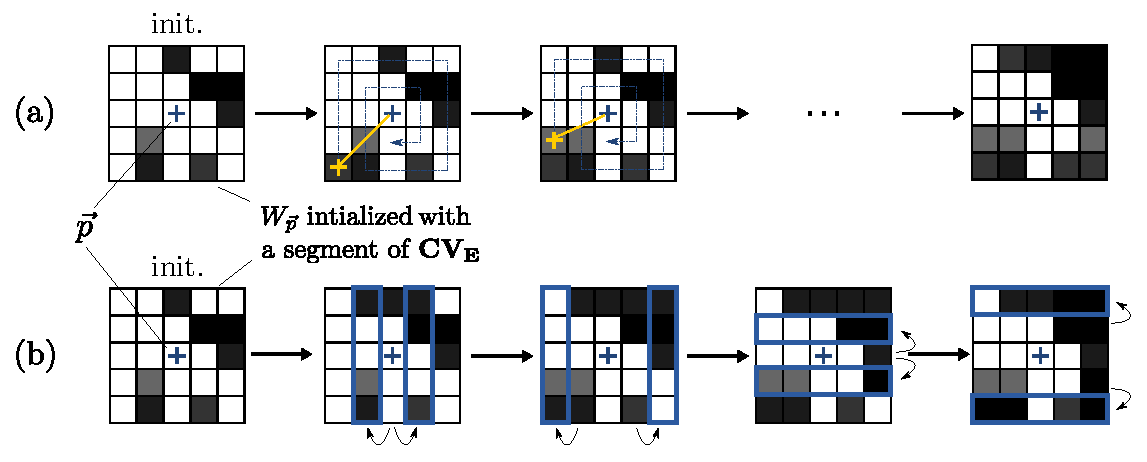
\includegraphics[scale=0.65]{media/error_propagation.pdf}
	\end{center}
	\caption{Step-by-step visualization of the error propagation matrix calculation. The top figure (a) visualizes the calculation as given in equation \ref{eqn:error_matrix_bresenham}, (b) shows the calculation resulting from the approximation in equation \ref{eqn:error_matrix_approx}. In (a) the values from the edge image (black pixels correspond to edges) are multiplied along a line starting from the center pixel $\vec p$ (blue) to the target pixel (yellow). Choosing the target pixels along a spiral path allows the matrix to be updated in-place. The approximation in (b) can be calculated by in-place multiplication of neighboring columns and rows respectively starting from the center.}
	\label{fig:error_propagation}
\end{figure}

The entries of the normalized propagation matrix are given as
\begin{equation*}
	w_{ij} = \frac{w_{ij}'}{\sum_{i, j} w_{ij}'}
\end{equation*}

\section{Propagation matrix performance}

\begin{figure}[t]
\begin{center}
 \textbf{Apartment scene}\\
 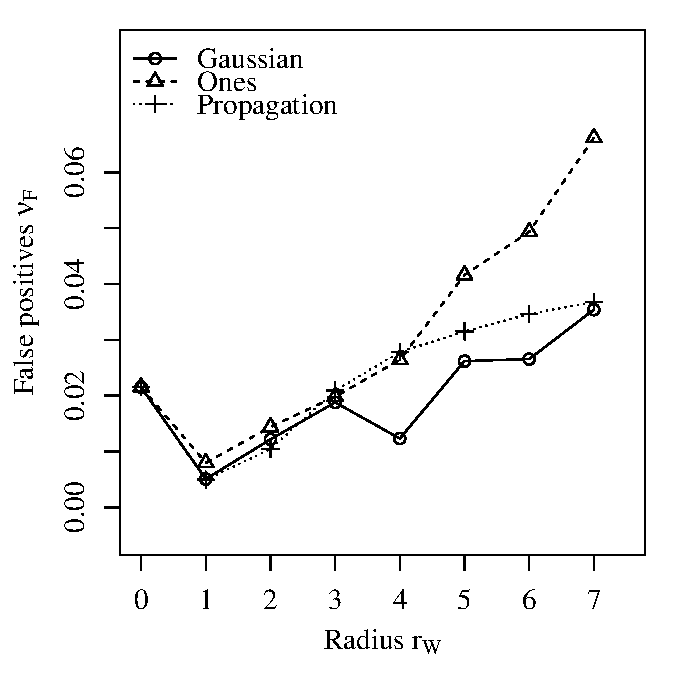
\includegraphics[width=0.475\textwidth]{results/matrices/propmat_apartment_mF.pdf}
 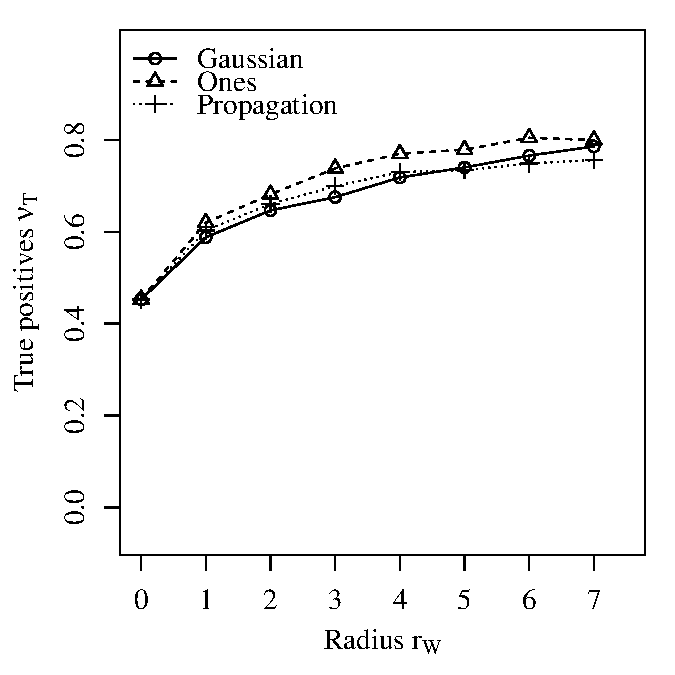
\includegraphics[width=0.475\textwidth]{results/matrices/propmat_apartment_mT.pdf}
 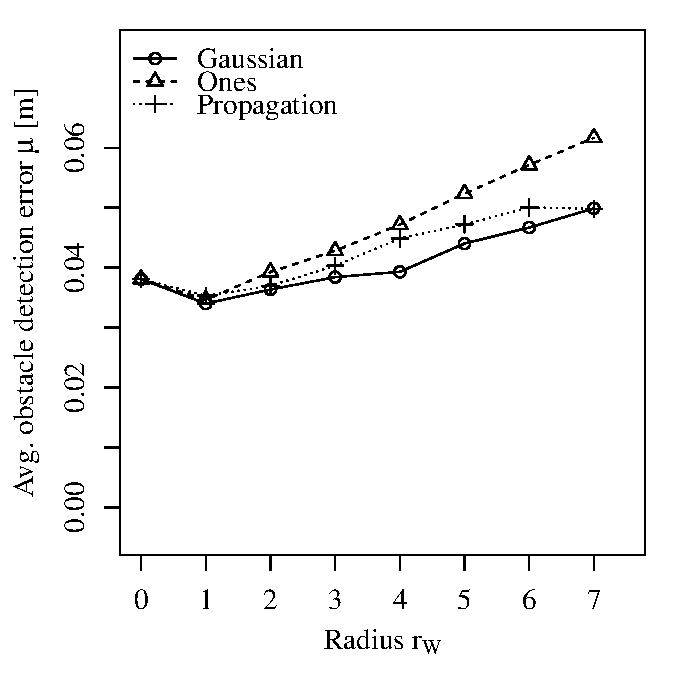
\includegraphics[width=0.475\textwidth]{results/matrices/propmat_apartment_meanDist.pdf}
 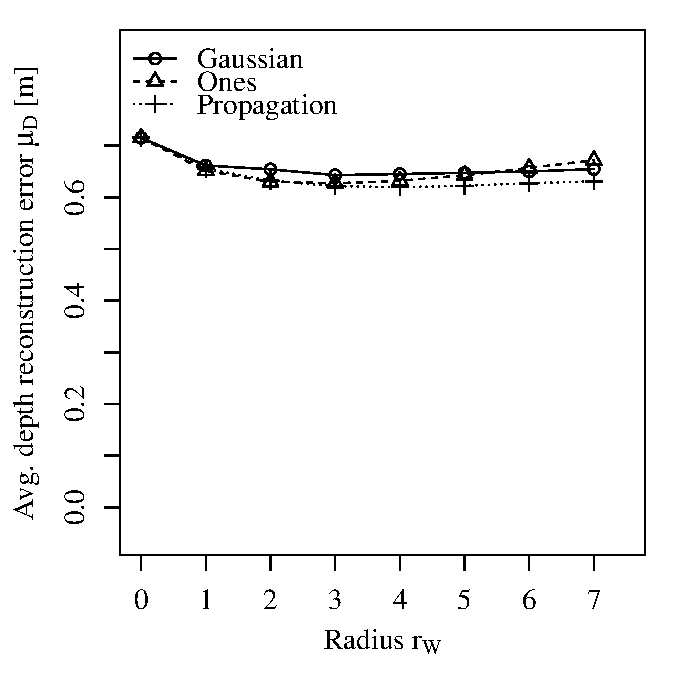
\includegraphics[width=0.475\textwidth]{results/matrices/propmat_apartment_avgNettoMean.pdf}
\end{center}
\caption{Results for varying propagation matrices $W_{\vec p}$ in the apartment scene.}
\label{fig:results_propagation_apa}
\end{figure}

\begin{figure}[t]
\begin{center}
 \textbf{Laboratory scene}\\
 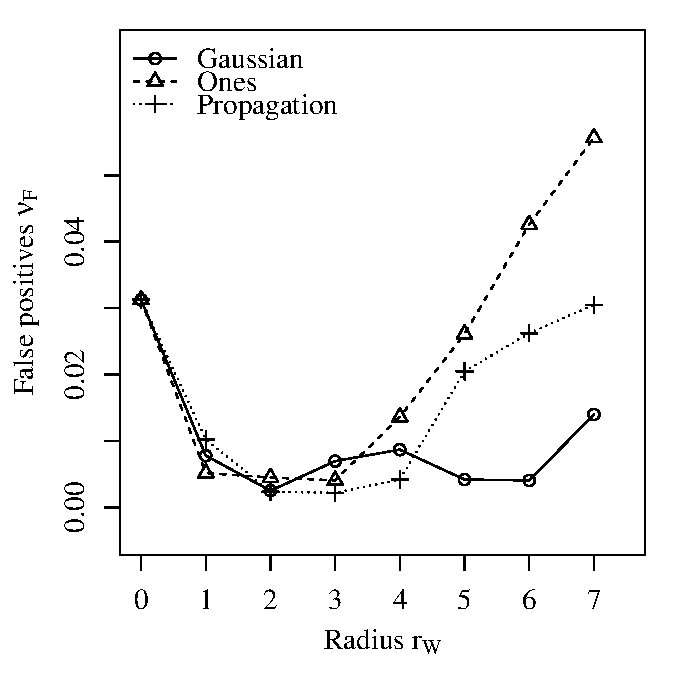
\includegraphics[width=0.475\textwidth]{results/matrices/propmat_laboratory_mF.pdf}
 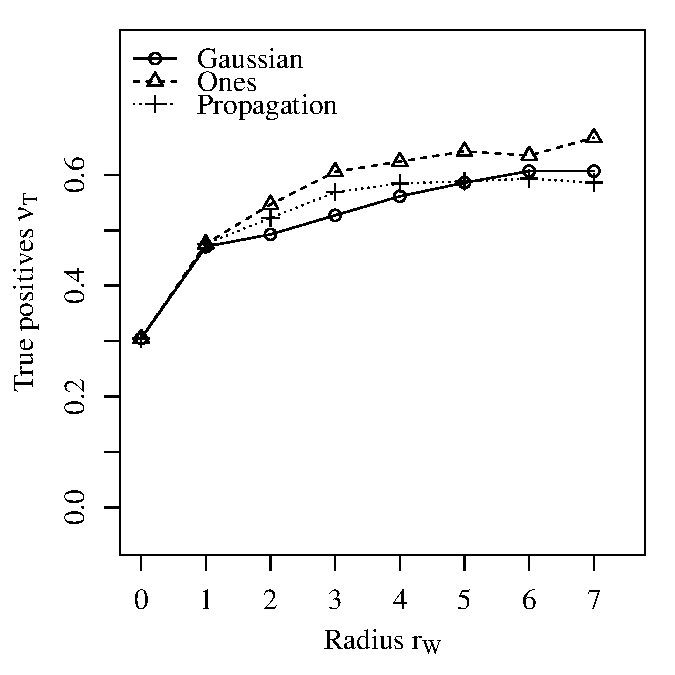
\includegraphics[width=0.475\textwidth]{results/matrices/propmat_laboratory_mT.pdf}
 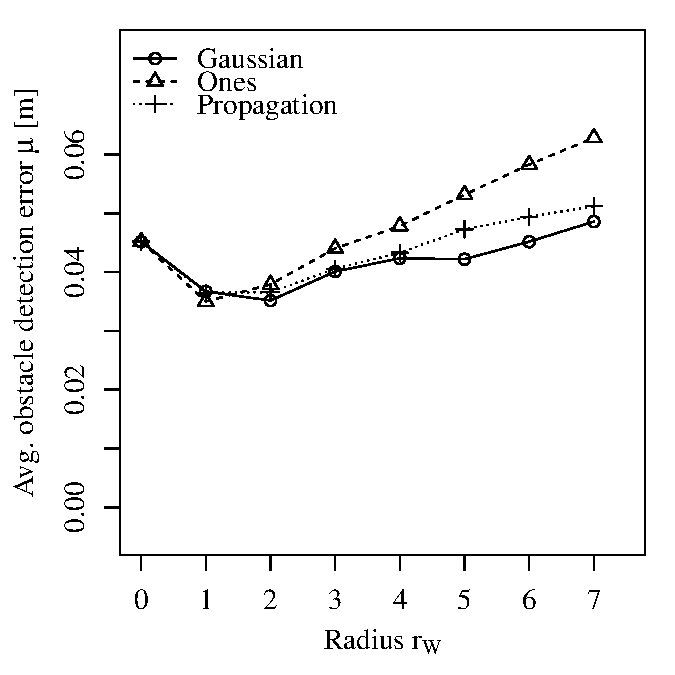
\includegraphics[width=0.475\textwidth]{results/matrices/propmat_laboratory_meanDist.pdf}
 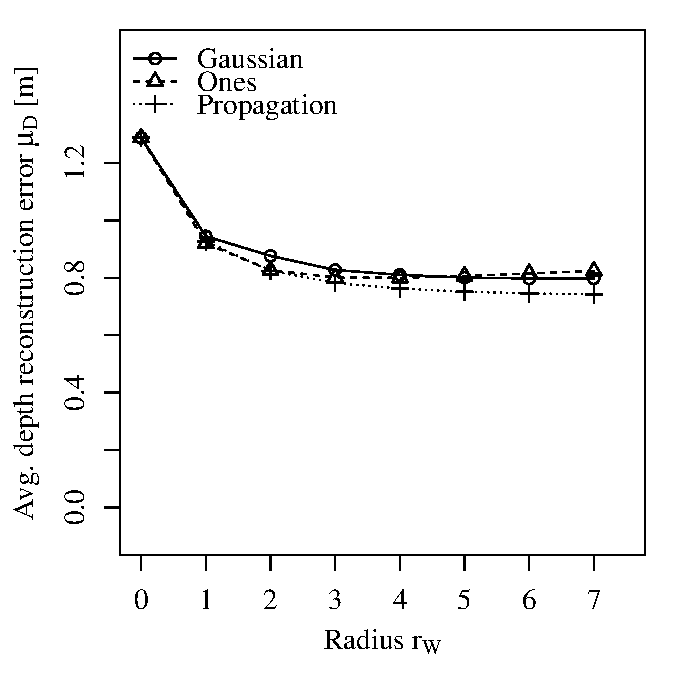
\includegraphics[width=0.475\textwidth]{results/matrices/propmat_laboratory_avgNettoMean.pdf}
\end{center}
\caption{Results for varying propagation matrices $W_{\vec p}$ in the laboratory scene.}
\label{fig:results_propagation_lab}
\end{figure}

\label{sec:results_propagation}

\paragraph{Experiment description:} The tests in this section are performed in order to determine the best type and radius $r_W$ of the error propagation matrix $W_\vec{p}$. Note that this test is performed using the (non-realtime) author's personal reference implementation (not described in this thesis), as support for different types of error propagation matrices and varying radii was removed from the optimized implementation.

The experiment is conducted in the simulated environments described in section \ref{sec:experiments}. In the test both the propagation matrix radius $m \in \{0, \ldots, 7\}$ and its type are varied. The types include a discrete Gaussian filter kernel (approximated using a binomial filter kernel, dubbed ``Gaussian''), a box filter (matrix of ones, dubbed ``Ones''), and the error propagation matrix as described above (dubbed ``Propagation'').

\paragraph{Results:} The results of the this experiment can be seen in figures \ref{fig:results_propagation_apa} and \ref{fig:results_propagation_lab}. One can see that for $r_W > 0$ the relative count of false positives $\nu_F$ first decreases but increases again for larger $r_W$. The same is true for the average obstacle detection error $\mu$. The relative count of true positives $\nu_T$ increases with increasing $r_W$. An extraordinarily high increase in $\nu_T$ and (along with a large drop in $\nu_F$ and $\mu_D$) can be seen in the step from $r_W = 0$ to $r_W = 1$).

Generally speaking there is no large difference in the performance of the different propagation matrix types. Yet the ``Ones''-matrix tendentially shows the worst performance and the ``Propagation''-matrices have a slightly superior depth reconstruction performance for large $r_W$.

A $3 \times 3$ (radius $r_W = 1$) binomial filter kernel was chosen for the optimized implementation: Larger radii increase the run time and do not necessarily yield a higher obstacle detection quality. The propagation matrices described above were not used, as they introduce an additional calculation step and (in contrast to the binomial kernel) are not separable and not space-invariant.

\chapter{Source code}

This appendix contains some excerpts of the source code at key points in the algorithm. Note that the code has been slightly simplified for illustration purposes. Thus each code snippet is accompanied by a reference to its location in the ``real source code''.

\section{Error stack calculation}

This section contains the code used for the error stack calculation as described in section \ref{sec:error_stack_sse}.

\subsection{Horizontal interpolation}

\label{code:horz_interpolation}

{\footnotesize Code located in \texttt{FlowSIMD-1-0/src/ErrorStack.C::\_ErrorstackInterpolateHorz}}

\lstinputlisting{code/errorstack_horz.c}

\subsection{Vertical interpolation}

\label{code:vert_interpolation}

{\footnotesize Code located in \texttt{FlowSIMD-1-0/src/ErrorStack.C::\_ErrorstackInterpolateVert}}

\lstinputlisting{code/errorstack_vert.c}

\section{Gauss template accumulation}

\label{code:gauss}

{\footnotesize Code located in \texttt{FlowSIMD-1-0/src/ObstacleMap.C::additiveBlitInline}}

This code is used for accumulating the gauss templates at a certain $x$-$y$-position in the local environment map. The attribute \texttt{flip} specifies whether the template is to be placed in quadrants 2 or 4 (see figure \ref{fig:gaussian_distribution_symmetries}).

\lstinputlisting{code/gauss.c}

\end{appendix}


\bibliography{bibliography}
\bibliographystyle{plainnat}

\cleardoublepage

\pagestyle{empty}

Hiermit versichere ich, dass ich diese Bachelorarbeit selbständig bearbeitet habe. Ich habe keine anderen als die angegebenen Quellen und Hilfsmittel benutzt und entsprechende Zitate kenntlich gemacht.
\begin{center}
\vspace{1.5cm}
\begin{tabular}{l l l}
  Bielefeld, \insertdate & \hspace{0.5cm} & \hspace{6.5cm} \\
  \hline
  \footnotesize \textsc{Datum} & & \footnotesize \textsc{\insertauthor}
\end{tabular}
\end{center}

\end{document}
